\documentclass{cmspaper}
\usepackage{graphicx}
\usepackage{amsmath}
\usepackage{amssymb}
\usepackage{subfigure}
\usepackage{multirow}
\usepackage[pdfborder=0 0 0,
            colorlinks,
            urlcolor = blue,
            linkcolor = black,
            citecolor = black,
            menucolor = black,]
           {hyperref}
%% \usepackage[colorlinks]{hyperref}
%% \usepackage{url}
\usepackage[toc,page]{appendix}
\renewcommand{\appendixname}{Appendix}
%% \renewcommand{\appendixtocname}{List of appendices}

% % useful definitions

% processes
\def\dyee {\ensuremath{Z/\gamma^*\to ee}}
\def\dymm {\ensuremath{Z/\gamma^*\to\mu\mu}}
\def\dytt {\ensuremath{Z/\gamma^*\to\tau\tau}}
\def\zee {\ensuremath{Z\to ee}}
\def\zmm {\ensuremath{Z\to\mu\mu}}
\def\ztt {\ensuremath{Z\to\tau\tau}}
\def\ttbar {\ensuremath{t\bar{t}}}
\def\wwll {\ensuremath{WW\to l^+l^-}}
\def\wwlulu{\ensuremath{WW\to l^+\nu l^-\bar{\nu}}}
\def\ww {\ensuremath{WW}}
\def\hww {\ensuremath{H\to WW}}
\def\wz{\ensuremath{WZ}}
\def\zz{\ensuremath{ZZ}}
\def\wgamma{\ensuremath{W\gamma}}
\def\wjets{\ensuremath{W+}jets} 
\def\tw{\ensuremath{tW}} 
\def\singletopt{\ensuremath{t} ($t$-chan)} 
\def\singletops{\ensuremath{t} ($s$-chan)} 
\def\all{all}
\def\ee{\ensuremath{ee}}
\def\emu{\ensuremath{e\mu}}
\def\mm{\ensuremath{\mu\mu}}

%units
\newcommand{\TeV}{\ensuremath{\mathrm{Te\kern -0.1em V}}}
\newcommand{\GeV}{\ensuremath{\mathrm{Ge\kern -0.1em V}}}

%others
\def\pt{\ensuremath{p_T}}
\def\ipb{pb\ensuremath{^{-1}}}
\def\ifb{fb\ensuremath{^{-1}}}
\def\et{\ensuremath{E_T}}
\def\met{\ensuremath{E\!\!\!\!/_T}}
\def\fBrem{\ensuremath{f_{\rm brem}}}
\def\pin{\ensuremath{p_{\rm in}}}
\def\pout{\ensuremath{p_{\rm out}}}

\newcommand{\CLs}{\ensuremath{CL_\mathrm{s}}}
\newcommand{\CLb}{\ensuremath{CL_\mathrm{b}}}
\newcommand{\CLsb}{\ensuremath{CL_\mathrm{s+b}}}

\newcommand{\GeV}{\ensuremath{\mathrm{Ge\kern -0.1em V}}}
\newcommand{\TeV}{\ensuremath{\mathrm{Te\kern -0.1em V}}}
\newcommand{\TeVcc}{\ensuremath{\,\mathrm{Te\kern -0.1em V\!/c}^2}}
\newcommand{\GeVcc}{\ensuremath{\,\mathrm{Ge\kern -0.1em V\!/c}^2}}
\newcommand{\MeVcc}{\ensuremath{\,\mathrm{Me\kern -0.1em V\!/c}^2}}
\newcommand{\GeVc}{\ensuremath{\mathrm{Ge\kern -0.1em V}\!/c}}
\newcommand{\nanob}{\mbox{{\rm ~nb}~}}
\newcommand{\fb}{\ensuremath{\mathrm{fb}}}
\newcommand{\pb}{\ensuremath{\mathrm{pb}}}
\newcommand{\ifb}{\ensuremath{\mathrm{fb^{-1}}}}
\newcommand{\ipb}{\ensuremath{\mathrm{pb^{-1}}}}
\newcommand{\grad}{\ensuremath{^{\circ}}}
%
% Special user made math symbols
%
\newcommand{\lsim}{\raisebox{-1.5mm}{$\:\stackrel{\textstyle{<}}{\textstyle{\sim}}\:$}}
\newcommand{\gsim}{\raisebox{-1.5mm}{$\:\stackrel{\textstyle{>}}{\textstyle{\sim}}\:$}}

% particles

\newcommand{\pipm}{\ensuremath{\pi^{\pm}}}
\newcommand{\pizero}{\ensuremath{\pi^{0}}}
\newcommand{\Hi}{\ensuremath{\mathrm{H}}}
\newcommand{\W}{\ensuremath{\mathrm{W}}}
\newcommand{\Wjets}{\ensuremath{\mathrm{W+jets}}}
\newcommand{\Zjets}{\ensuremath{\mathrm{Z+jets}}}
\newcommand{\Wt}{\ensuremath{\mathrm{Wt}}}
\newcommand{\Wstar}{\ensuremath{\mathrm{W}^{*}}}
\newcommand{\Wparenthesisstar}{\ensuremath{\mathrm{W}^{(*)}}}
\newcommand{\WW}{\ensuremath{\W^+\W^-}}
\newcommand{\Z}{\ensuremath{\mathrm{Z}}}
\newcommand{\Zstar}{\ensuremath{\mathrm{Z}^{*}}}
\newcommand{\Astar}{\ensuremath{\mathrm{\gamma}^{*}}}
\newcommand{\ZZ}{\ensuremath{\Z\Z}}
\newcommand{\WZ}{\ensuremath{\W\Z}}
\newcommand{\Wgstar}{\ensuremath{\W\Astar}}
\newcommand{\E}{\ensuremath{\mathrm{e}}}
\newcommand{\Ep}{\ensuremath{\mathrm{e}^{+}}}
\newcommand{\Em}{\ensuremath{\mathrm{e}^{-}}}
\newcommand{\Epm}{\ensuremath{\mathrm{e}^{\pm}}}
\newcommand{\Emp}{\ensuremath{\mathrm{e}^{\mp}}}
\newcommand{\M}{\ensuremath{\mu}}
\newcommand{\Mp}{\ensuremath{\mu^{+}}}
\newcommand{\Mm}{\ensuremath{\mu^{-}}}
\newcommand{\Mpm}{\ensuremath{\mu^{\pm}}}
\newcommand{\Mmp}{\ensuremath{\mu^{\mp}}}
\newcommand{\Tau}{\ensuremath{\tau}}
\newcommand{\Nu}{\ensuremath{\nu}}
\newcommand{\Nubar}{\ensuremath{\bar{\nu}}}
\newcommand{\Lep}{\ensuremath{\ell}}
\newcommand{\Lepp}{\ensuremath{\ell^{+}}}
\newcommand{\Lepm}{\ensuremath{\ell^{-}}}
\newcommand{\Lprime}{\ensuremath{\Lep^{\prime}}}
\newcommand{\Prot}{\ensuremath{\mathrm{p}}}
\newcommand{\Pbar}{\ensuremath{\bar{\mathrm{p}}}}
\newcommand{\PP}{\Prot\Prot}
\newcommand{\PPbar}{\Prot\Pbar}
\newcommand{\ttbar}{\ensuremath{\mathrm{t}\bar{\mathrm{t}}}}
\newcommand{\qq}{\ensuremath{\mathrm{q}\mathrm{q}}}
%\newcommand{\bbbar}{\ensuremath{\mathrm{b}\bar{\mathrm{b}}}}
\newcommand{\Wtb}{\ensuremath{\W\mathrm{t}\mathrm{b}}}
\newcommand{\Top}{\ensuremath{\mathrm{t}}}
\newcommand{\Bot}{\ensuremath{\mathrm{b}}}
\newcommand{\Atop}{\ensuremath{\bar{\mathrm{t}}}}
\newcommand{\Abot}{\ensuremath{\bar{\mathrm{b}}}}
% arrow
\newcommand{\To}{\ensuremath{\rightarrow}}

% masses
\newcommand{\mHi}{\ensuremath{m_{\mathrm{H}}}}
\newcommand{\mW}{\ensuremath{m_{\mathrm{W}}}}
\newcommand{\mZ}{\ensuremath{m_{\mathrm{Z}}}}
\newcommand{\mll}{\ensuremath{m_{\Lep\Lep}}}
\newcommand{\mt}{\ensuremath{m_{\mathrm{T}}}}

% kinematics
\newcommand{\pt}{\ensuremath{p_\mathrm{T}}}
\newcommand{\ptveto}{\ensuremath{\pt^\mathrm{veto}}}
\newcommand{\ptl}{\ensuremath{p_\perp^{\Lep}}}
\newcommand{\ptlmax}{\ensuremath{p_{\mathrm{T}}^{\Lep,\mathrm{max}}}}
\newcommand{\ptlmin}{\ensuremath{p_{\mathrm{T}}^{\Lep,\mathrm{min}}}}
\newcommand{\met}{\ensuremath{\Et^{\mathrm{miss}}}}
\newcommand{\delphill}{\ensuremath{\Delta\phi_{\Lep\Lep}}}
\newcommand{\deletall}{\ensuremath{\Delta\eta_{\Lep\Lep}}}
\newcommand{\delphimetl}{\ensuremath{\Delta\phi_{\met\Lep}}}
\newcommand{\Et}{\ensuremath{E_\mathrm{T}}}
\newcommand{\delR}{\ensuremath{\Delta R}}
\newcommand{\Eta}{\ensuremath{\eta}}

%efficiencies
\newcommand{\effsig}{\ensuremath{\varepsilon_{\mathrm{bkg}}^{\mathrm{S}}}}
\newcommand{\effnorm}{\ensuremath{\varepsilon_{\mathrm{bkg}}^{\mathrm{N}}}}
\newcommand{\Nsig}{\ensuremath{N_{\mathrm{bkg}}^{\mathrm{S}}}}
\newcommand{\Nnorm}{\ensuremath{N_{\mathrm{bkg}}^{\mathrm{N}}}}

% processes
\newcommand{\dyee}{\ensuremath{Z/\gamma^*\to ee}}
\newcommand{\dymm}{\ensuremath{Z/\gamma^*\to\mu\mu}}
\newcommand{\dytt}{\ensuremath{Z/\gamma^*\to\tau\tau}}
\newcommand{\dyll}{\ensuremath{Z/\gamma^*\to\ell\ell}}
\newcommand{\dy}{\ensuremath{Z/\gamma^*}}
\newcommand{\zee}{\ensuremath{Z\to ee}}
\newcommand{\zmm}{\ensuremath{Z\to\mu\mu}}
\newcommand{\ztt}{\ensuremath{Z\to\tau\tau}}
%\newcommand{\ttbar}{\ensuremath{t\bar{t}}}
\newcommand{\ppww}{\ensuremath{pp \to W^+W^-}}
\newcommand{\wwll}{\ensuremath{WW\to \ell^+\ell^-}}
\newcommand{\wwlnln}{\ensuremath{W^+W^-\to \ell^+\nu \ell^-\bar{\nu}}}
\newcommand{\ww}{\ensuremath{WW}}
\newcommand{\wwpm}{\ensuremath{W^+W^-}}
\newcommand{\hww}{\ensuremath{H\to W^+W^-}}
\newcommand{\wz}{\ensuremath{WZ}}
\newcommand{\zz}{\ensuremath{ZZ}}
\newcommand{\wgamma}{\ensuremath{W\gamma}}
\newcommand{\wjets}{\ensuremath{W+}jets} 
\newcommand{\tw}{\ensuremath{tW}} 
\newcommand{\singletopt}{\ensuremath{t} ($t$-chan)} 
\newcommand{\singletops}{\ensuremath{t} ($s$-chan)} 
\newcommand{\zx}{\ensuremath{\mathrm{DY/WZ/ZZ}}}
\newcommand{\zv}{\ensuremath{\mathrm{WZ/ZZ}}}
\newcommand{\z}{\ensuremath{\mathrm{Z}}}
\newcommand{\routin}{\ensuremath{R_{out/in}}}

%other 
\def\fixme{({\bf FixMe})}
\newcommand{\ee}{\ensuremath{ee}}
\newcommand{\emu}{\ensuremath{e\mu}}
\def\mm{\ensuremath{\mu\mu}}

% integrated luminosity
\newcommand{\intlumiSevenTeV}{4.92~\ifb}
\newcommand{\intlumiEightTeV}{1.62~\ifb}

%%%%%%%%%%%
%
\newcounter{myfootertablecounter}

\newcommand\myfootnotemark{%
  %\refstepcounter{footnote}%
  \addtocounter{footnote}{1}%
  \footnotemark[\thefootnote]%
}%

\newcommand\myfootnotetext[1]{%
  \addtocounter{myfootertablecounter}{1}
  \footnotetext[\value{myfootertablecounter}]{#1}
}

% from now on, myfootnote has to be used rather than footnote to
% adapt the myfootercounter
\newcommand\myfootnote[1]{%
  \addtocounter{myfootertablecounter}{1}
  \footnote{#1}
}%



\setcounter{topnumber}{1}
\setcounter{bottomnumber}{1}

%===================================================================================================
\begin{document}
\begin{titlepage}

  \analysisnote{2011/XXX}

  \date{\today}

  \title{Shape analysis for Higgs searches in di-lepton final state}

  \begin{Authlist}
%
A.~Apyan~\Aref{ 2 },
W.~Andrews~\Aref{ 4 }, 
D.~Barge~\Aref{ 3 }, 
L.~Bauerdick~\Aref{ 1 }, 
G.~Bauer~\Aref{ 2 },
J.~Bendavid~\Aref{ 2 },
K.~Burkett~\Aref{ 1 }, 
E.~Butz~\Aref{ 2 },
C.~Campagnari~\Aref{ 3 }, 
G.~Cerati~\Aref{ 4 },
M.~Chan~\Aref{ 2 },
V.~Dutta~\Aref{ 2 },
D.~Evans~\Aref{ 4 }, 
I.~Fisk~\Aref{ 1 }, 
G.~G\'omez-Ceballos~\Aref{ 2 },
Y.~Gao~\Aref{ 1 }, 
F.~Golf~\Aref{ 4 }, 
M.~Goncharov~\Aref{ 2 },
O.~Gutsche~\Aref{ 1 }, 
K.~Hahn~\Aref{ 2 },
P.~Harris~\Aref{ 6 },
B.~Hooberman~\Aref{ 1 },
S.~Jindariani~\Aref{ 1 },
M.~Klute~\Aref{ 2 },
D.~Kovalskyi~\Aref{ 3 }~\Aref{ 6 }, 
I.~Kravchenko~\Aref{ 5 },
V.~Krutelyov~\Aref{ 3 }, 
A.~Levin~\Aref{ 2 }, 
I.~MacNeill~\Aref{ 4 },
S.~Nahn~\Aref{ 2 },
S.~Padhi~\Aref{ 4 }, 
C.~Paus~\Aref{ 2 },
D.~Ralph~\Aref{ 2 },
F.~Stoeckli~\Aref{ 2 },
K.~Sumorok~\Aref{ 2 },
K.~Sung~\Aref{ 2 },
S.~Tkaczyk~\Aref{ 1 },
Y.~Tu~\Aref{ 4 }, 
F.~W\"urthwein~\Aref{ 4 }, 
R.~Wolf~\Aref{ 2 },
S.~Xie~\Aref{ 2 },
A.~Yagil~\Aref{ 4 }, 
M.~Yang~\Aref{ 2 },
J.~Yoo~\Aref{ 4 },
M.~Zanetti~\Aref{ 2 }
%
\end{Authlist}
\Anotfoot{ 1 }{Fermilab National Accelerator Laboratory, Batavia, USA}
\Anotfoot{ 2 }{Laboratory for Nuclear Science, Massachusetts Institute of Technology, Cambridge, USA}
\Anotfoot{ 3 }{University of California, Santa Barbara, Santa Barbara, USA}
\Anotfoot{ 4 }{University of California, San Diego, San Diego, USA}
\Anotfoot{ 5 }{University of Nebraska-Lincoln, USA}
\Anotfoot{ 6 }{CERN, Switzerland}


  \begin{abstract}
    This note describes implementation details and treatment of
    systematic uncertainties of the multivariate shape analysis for
    Higgs boson searches in the $\WW \to 2\ell2\nu$ and $\ZZ \to
    2\ell2\nu$ final states.
  \end{abstract} 

\end{titlepage}
\tableofcontents
\listoftables
\listoffigures
\newpage 

%===================================================================================================
\section{Introduction}
  \label{sec:overview}
  Precision measurement of the gauge boson couplings is a well known
method to look for physics beyond the Standard Model. In the case of
the triple gauge boson couplings, new physics contributions can be
expressed in the form of an effective Lagrangian. The most general
form of such a Lagrangian has 14 complex couplings (7 for $WWZ$ and 7 for
$WW\gamma$). Assuming electromagnetic gauge invariance, and C and P
symmetry conservation that number is reduced to five:
$\Delta\kappa_Z$, $\Delta g^Z_1$, $\Delta\kappa_{\gamma}$, $\lambda_Z$
and $\lambda_{\gamma}$. Applying gauge constraints:
\begin{align}
  \Delta\kappa_Z &= \Delta g^Z_1- \Delta\kappa_{\gamma}\tan^2\theta_W \\
  \lambda_Z &= \lambda_{\gamma}
\end{align}
further reduces the number of independent couplings to three. In the
Standard Model all five couplings are zero. 
 
CMS performed a first measurement of the anomalous couplings with
35/pb of data at 7 TeV~\cite{blah}. The measurement was performed with
and without a form factor that helps to avoid unitarity violation by
introducing an effective cutoff scale where a coupling is switched
off.  In this study we have two orders of magnitude more data and
experimental constraints on the couplings are more stringent then the
unitarity constraint. Therefore all the anomalous couplings are
form-factor free.

This analysis is based on the $W^+W^-$ production cross-section
measurement in $\intlumi$ of $pp$ collision data at $\sqrt{s} = $
7~$\TeV$ (the full 2011 dataset) \cite{ref:WWXS2011}. 

measurement~\cite{ref:WWXS2011}. Here we just briefly summarize the event
selection showing mostly kinematic requirements that may affect the
leading lepton pt distribution, which is used as a main observable.

The kinematic observable used in this analysis is 
the transverse momentum (\pt) of the leading lepton,
shown in Figure \ref{fig:pas_pt1_incl} after all event selections
have been applied.

\begin{figure}[hb]
\subfigure[Linear scale]{\label{subfig:pas_pt1_incl}
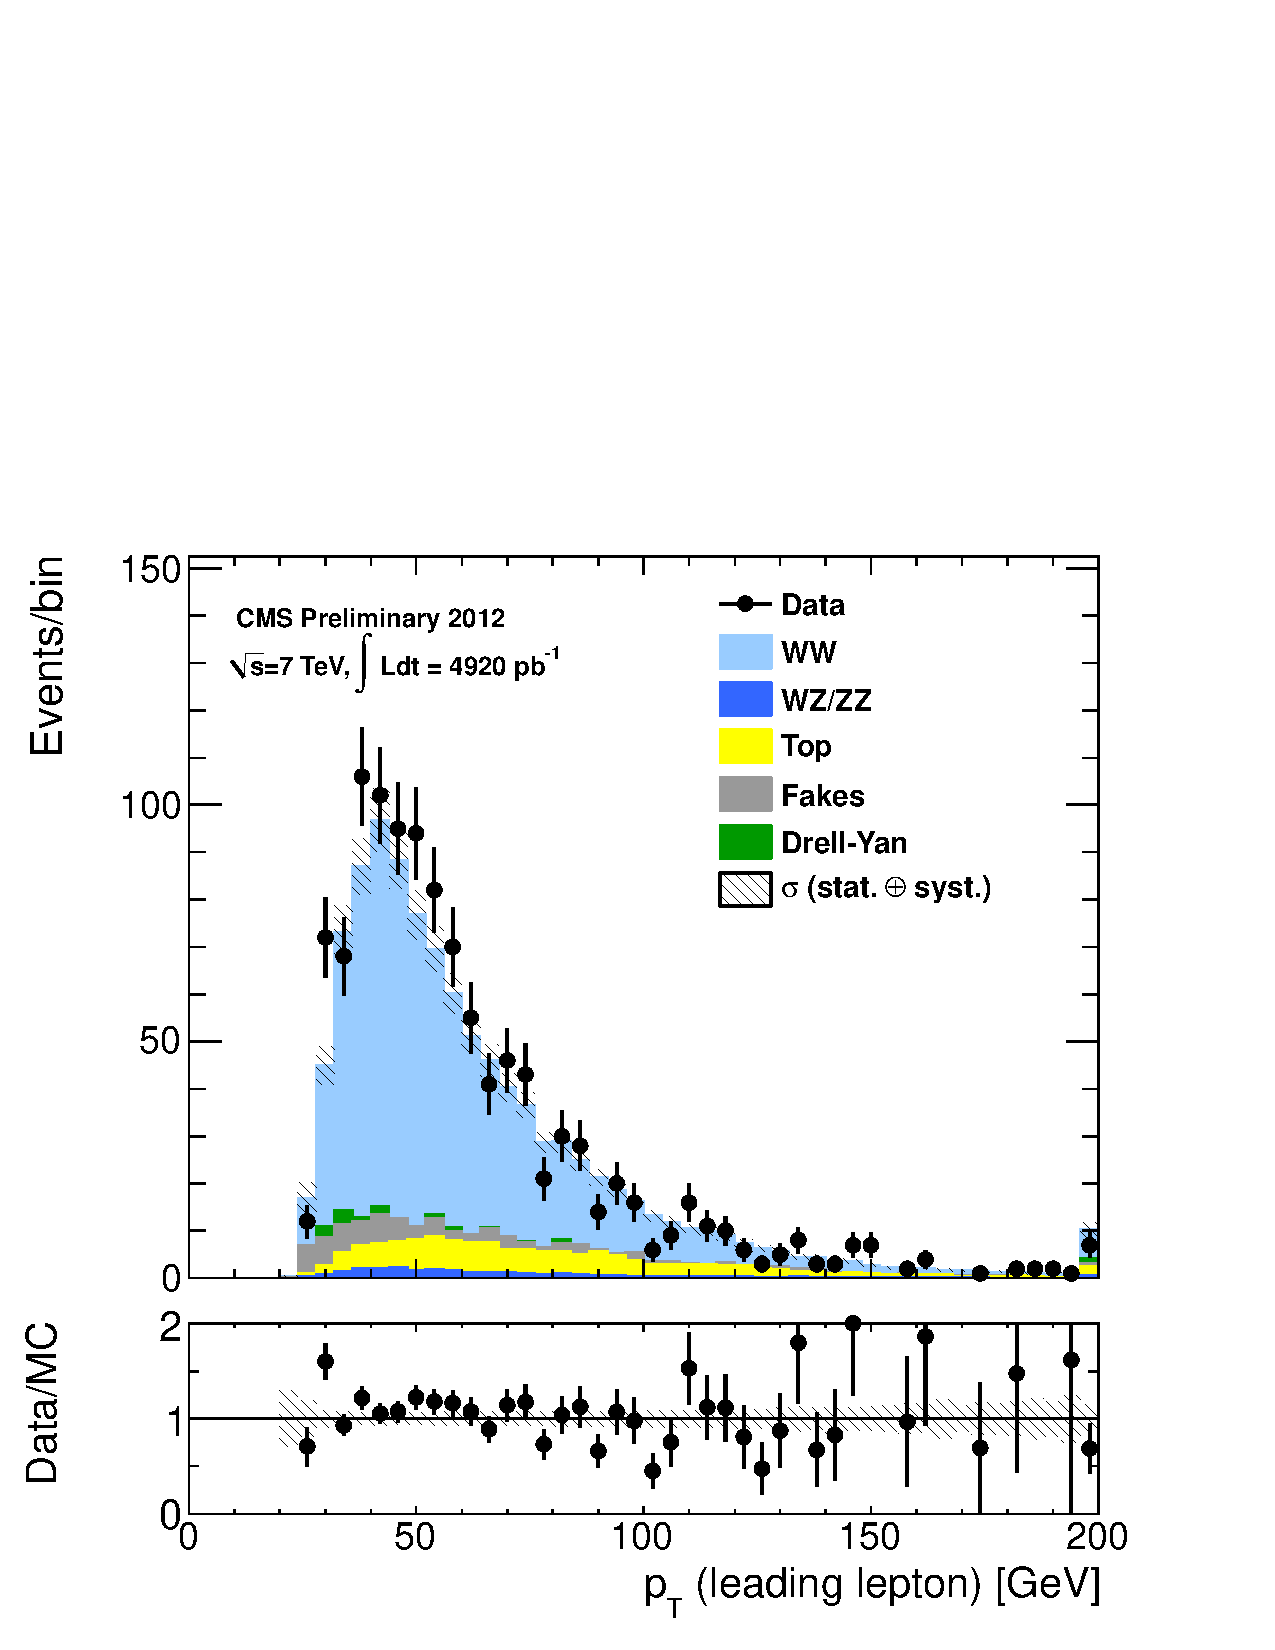
\includegraphics[width=.45\textwidth]{figures/pas_pt1_incl.pdf}}
\subfigure[Log scale]{\label{subfig:pas_pt1_incl_log}
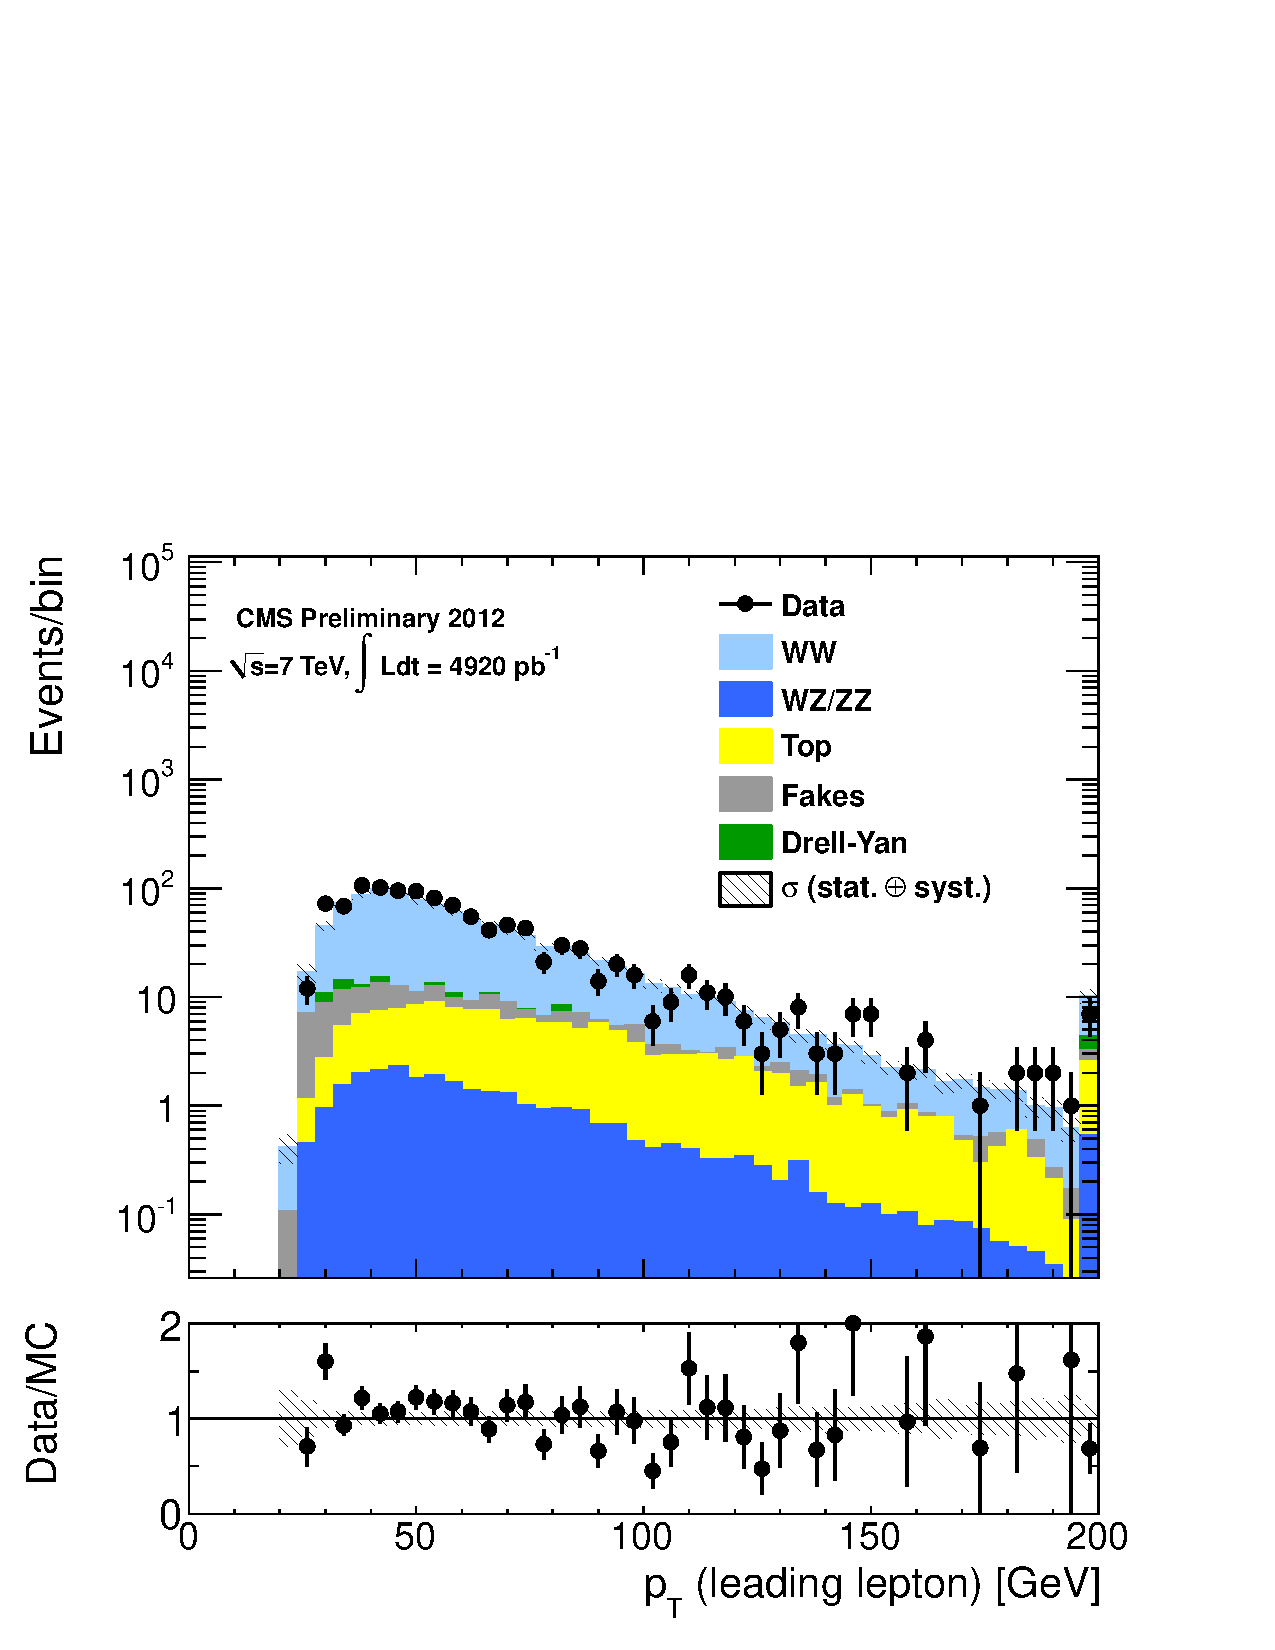
\includegraphics[width=.45\textwidth]{figures/pas_pt1_incl_log.pdf}}
\caption{Leading lepton \pt.}
\label{fig:pas_pt1_incl}
\end{figure}


  
\section{Statistical Methods}
  \label{sec:methods}
  Upper limits are derived on the product of the Higgs boson
production cross section and the $\Hi \to \WW (\Z\Z)$ branching fraction,
$\sigma_{\rm{H}} \times $BR($\Hi \to \WW (\Z\Z))$, with respect
to the SM expectation, i.e. $\sigma^{95\%}/\sigma^{SM}$. Two different
statistical methods are used, both using the same likelihood function
from the expected number of observed events modeled as a Poisson
random variable whose mean value is the sum of the contributions from
signal and background processes. The first method, known as $CL_{s}$,
is based on the hybrid Frequentist-Bayesian approach~\cite{cousins},
while the second one is based on Bayesian inference~\cite{bayesian}.
Both methods account for systematic uncertainties. Although not
identical, the upper limits obtained from both methods are similar. 
To perform the computation of the limits, the software packages
\texttt{RooStats}~\cite{rootstat} and \texttt{LandS}~\cite{lands} have 
been used. Whenever the same result was computed with both packages, the
results were found to agree.

\subsection{Systematic Uncertainties in Shape Analyses} 

There are three different ways to account for systematic uncertainties for a 
given source:
\begin{itemize}
  \item {\bf normalization uncertanty} - account only for the overall
    normalization assuming that the shape is perfectly known;
  \item {\bf statistical shape uncertainties} - account for limited
    number of events available for the shape extraction;
  \item {\bf shape variation uncertainties} - account for uncertainty
    on the shape itself.
\end{itemize}

Normalization uncertanties are the most straightforward to treat. They
are identical to those used in a cut-based analysis. To simplify the
analysis in some cases, such as background contributions with
large normalization uncertainties, it can be used as the only source of
systematic uncertainty ignoring the shape variation.

Statistical uncertainties on shape extraction are often
negligible. Only if the sample that is used for shape extraction has
small number of events this effect may become sizable. At the moment
only one of the two official tools used in the Higgs group supports
this type of uncertainty. There are a few ways to address this
issue. First we can use the tool that supports this type of
uncertainty (LandS) to estimate the impact of this effect on final
results. If it is small it can be ignored. If the effect is not
negligible we can split the sample in a number of categories and
perform multiple ``cut-based'' analyses. Both tools support that
option, but it is a bit complicated and should be used only if really
necessary.

Shape variation uncertainties are implemented using three shapes:
nominal, ``up''-alternative and ``down''-alternative. A single
nuisance parameter is used for all bins simultaneously.


\section{Implementation}
  \label{sec:implementation}
  LandS etc



\clearpage
\section{H$\to\WW \to 2\ell2\nu$ analysis}

\subsection{Systematic uncertainties}
  \label{sec:systematic_ww}
  The summary of the systematic effects and components that they affect considered 
in the $\Hi \to\WW \to 2\ell2\nu$ analysis is shown in Table~\ref{tab:hwwsyst}. 
To simplify, the following convention names are used to identify several signal 
and background processes: ggH (for $gg \to H$), qqWW (for $qq \to \WW$), ggWW 
(for $gg \to\WW$), VV (for $\WZ$ plus $\Z\Z$), Top (for $\ttbar$ plus $\tw$), 
Zjets (for $\dymm$ plus $\dyee$), Wjets (for $\Wjets$), Wgamma (for $\W+\gamma$) 
and Ztt (for $\dytt$).

\begin{table}[!ht]
\begin{center}
{\small
\begin{tabular}{|l|cccccccccccc|}
\hline
 Systematic Effect & ZH  & WH & qqH& ggH& qqWW & ggWW & VV & Top & Zjets & Wjets & Wgamma & Ztt\\
\hline
Higgs Theory       & X   & X  & X  & X  & -    & -    & -  & -   & -	 & -	 & -	  & - \\
PDF                & X   & X  & X  & X  & X    & X    & X  & -   & -	 & -	 & X	  & - \\
Lepton efficiency  & X   & X  & X  & X  & X    & X    & X  & X   & -	 & -	 & X	  & X \\
Lepton resolution  & X   & X  & X  & X  & X    & X    & X  & X   & -	 & -	 & X	  & X \\
MET resolution     & X   & X  & X  & X  & X    & X    & X  & X   & -	 & -	 & X	  & X \\
Jet Energy Scale   & X   & X  & X  & X  & X    & X    & X  & X   & -	 & -	 & X	  & X \\
\WW{}              & -   & -  & -  & -  & X    & X    & -  & -   & -	 & -	 & -	  & - \\
Top                & -   & -  & -  & -  & -    & -    & -  & X   & -	 & -	 & -	  & - \\
\dyll{}            & -   & -  & -  & -  & -    & -    & -  & -   & X	 & -	 & -	  & - \\
\wjets{}           & -   & -  & -  & -  & -    & -    & -  & -   & -	 & X	 & -	  & - \\
$\W\gamma$         & -   & -  & -  & -  & -    & -    & -  & -   & -	 & -	 & X	  & - \\
\dytt{}            & -   & -  & -  & -  & -    & -    & -  & -   & -	 & -	 & -	  & X \\
statistics         & X   & X  & X  & X  & X    & X    & X  & X   & X	 & X	 & X	  & X \\
\hline
\end{tabular}
\caption{Summary of the systematic effects and components that they affect considered in the 
$\Hi \to\WW \to 2\ell2\nu$ analysis.}
\label{tab:hwwsyst}
}
\end{center}
\end{table}

\subsubsection{Higgs Theoretical Uncertainties}
The theoretical systematic uncertainties on the signal yield is factorized into 
the product of two components. The first component is the uncertainty on the 
fraction of events categorized into the different jet bins and the effect of 
migrations across jet bins. The second component is the uncertainty on the 
lepton acceptance and the selection efficiency of all other cuts. The major
effect by far comes from the uncertainty on the normalization and it has been
described in detailed in~\cite{hww_eps, hww_lp}, following the prescriptions from
the Higgs cross section Yellow 
Report~\cite{LHCHiggsCrossSectionWorkingGroup:2011ti}.

The procedure to take into account a possible variation 
on the final discriminant variable due to the QCD renormalization ($\mu_R$) 
and scale ($\mu_F$) is to reweight the $gg \to H$ component with different k-factor
distributions. Since the normalization effects have their own factors, only a
shape variation is allowed. We the the ``up" variation as 
$\mu_R = 0.5\mu$ and $\mu_F =2.0\mu$ and the ``down" variation as 
$\mu_R = 2.0\mu$ and $\mu_F =0.5\mu$, being $\mu$ the nominal scale value. 
An example of the effect of this uncertainty is shown in Figure~\ref{fig:ggHsyst}. 
It is possible to see that the differences among the default distribution and the 
variations are very small.

\begin{figure}[!htbp]
\begin{center}
\subfigure[]{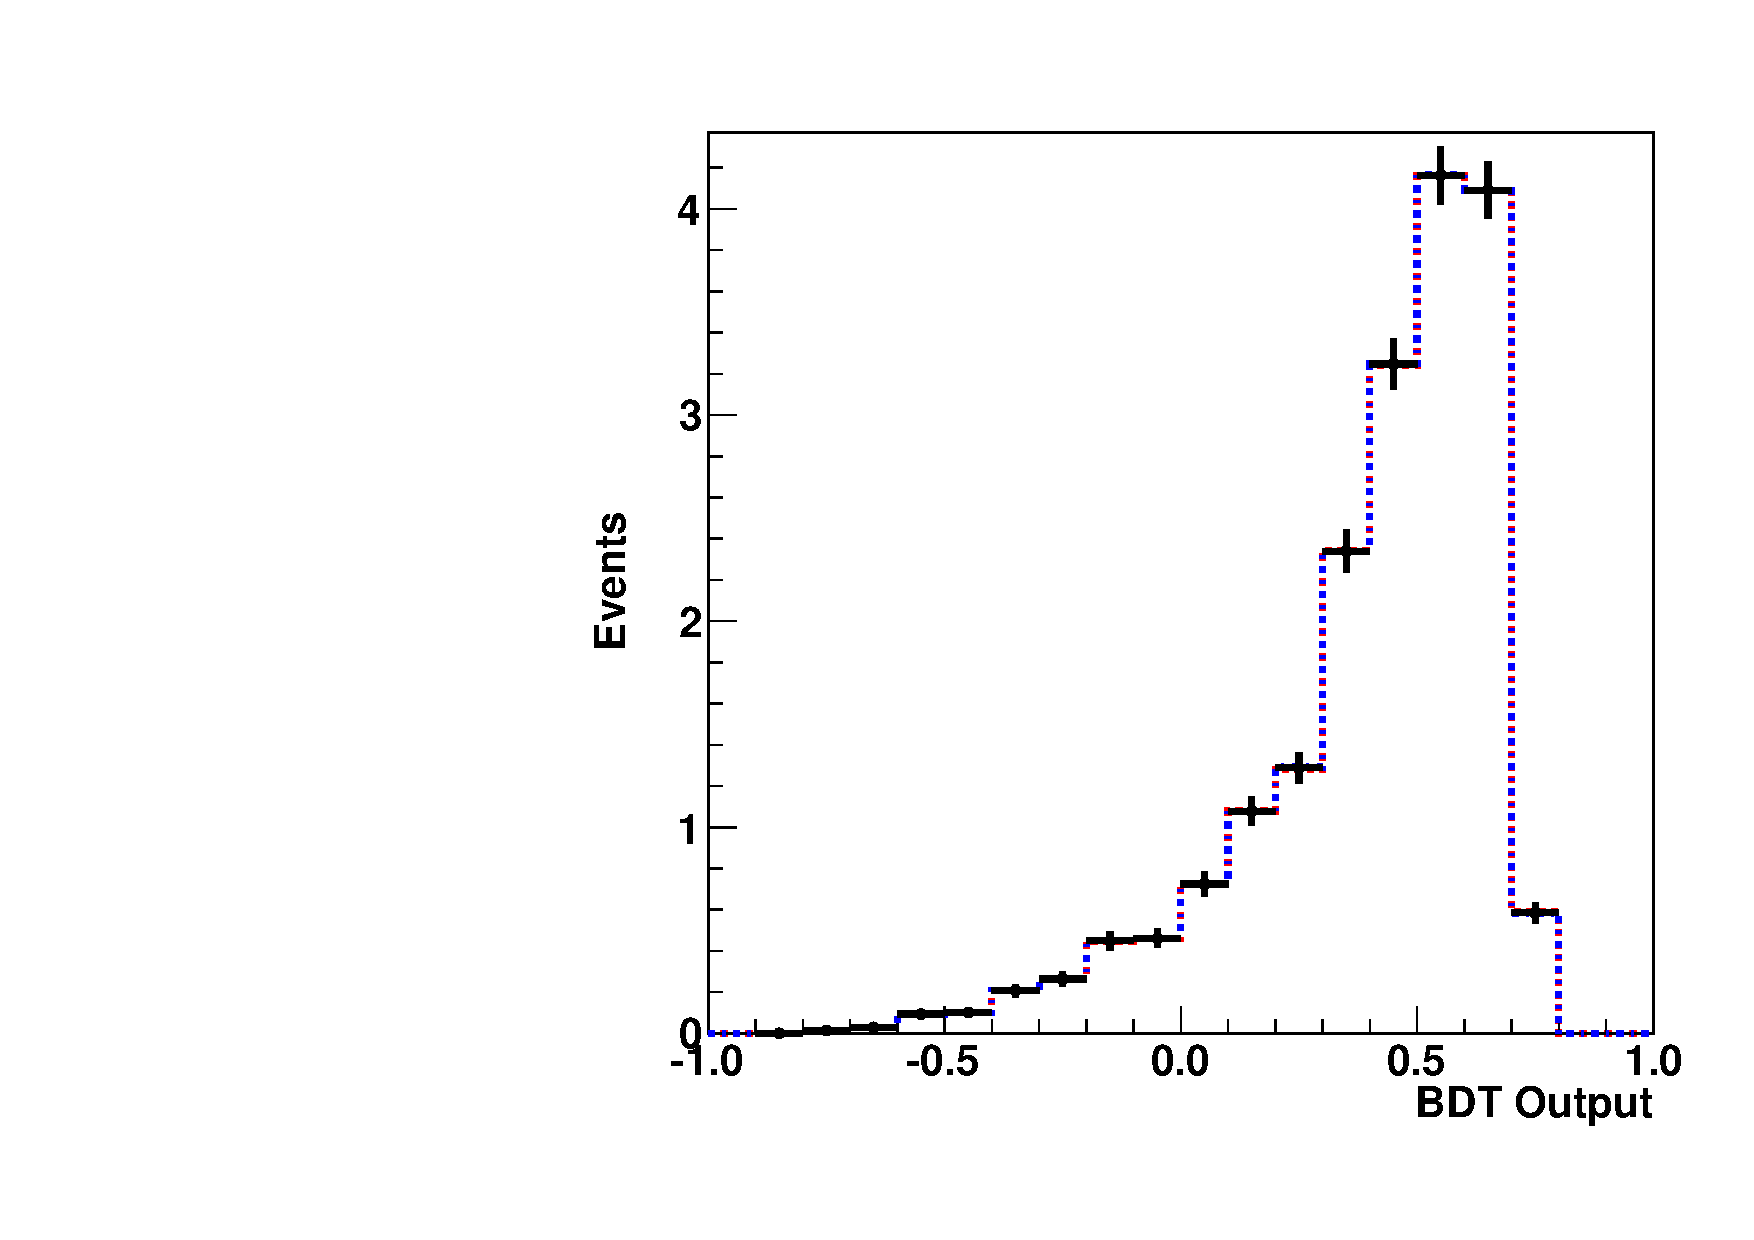
\includegraphics[width=0.49\textwidth]{figures/cvswwof_58.pdf}}
\subfigure[]{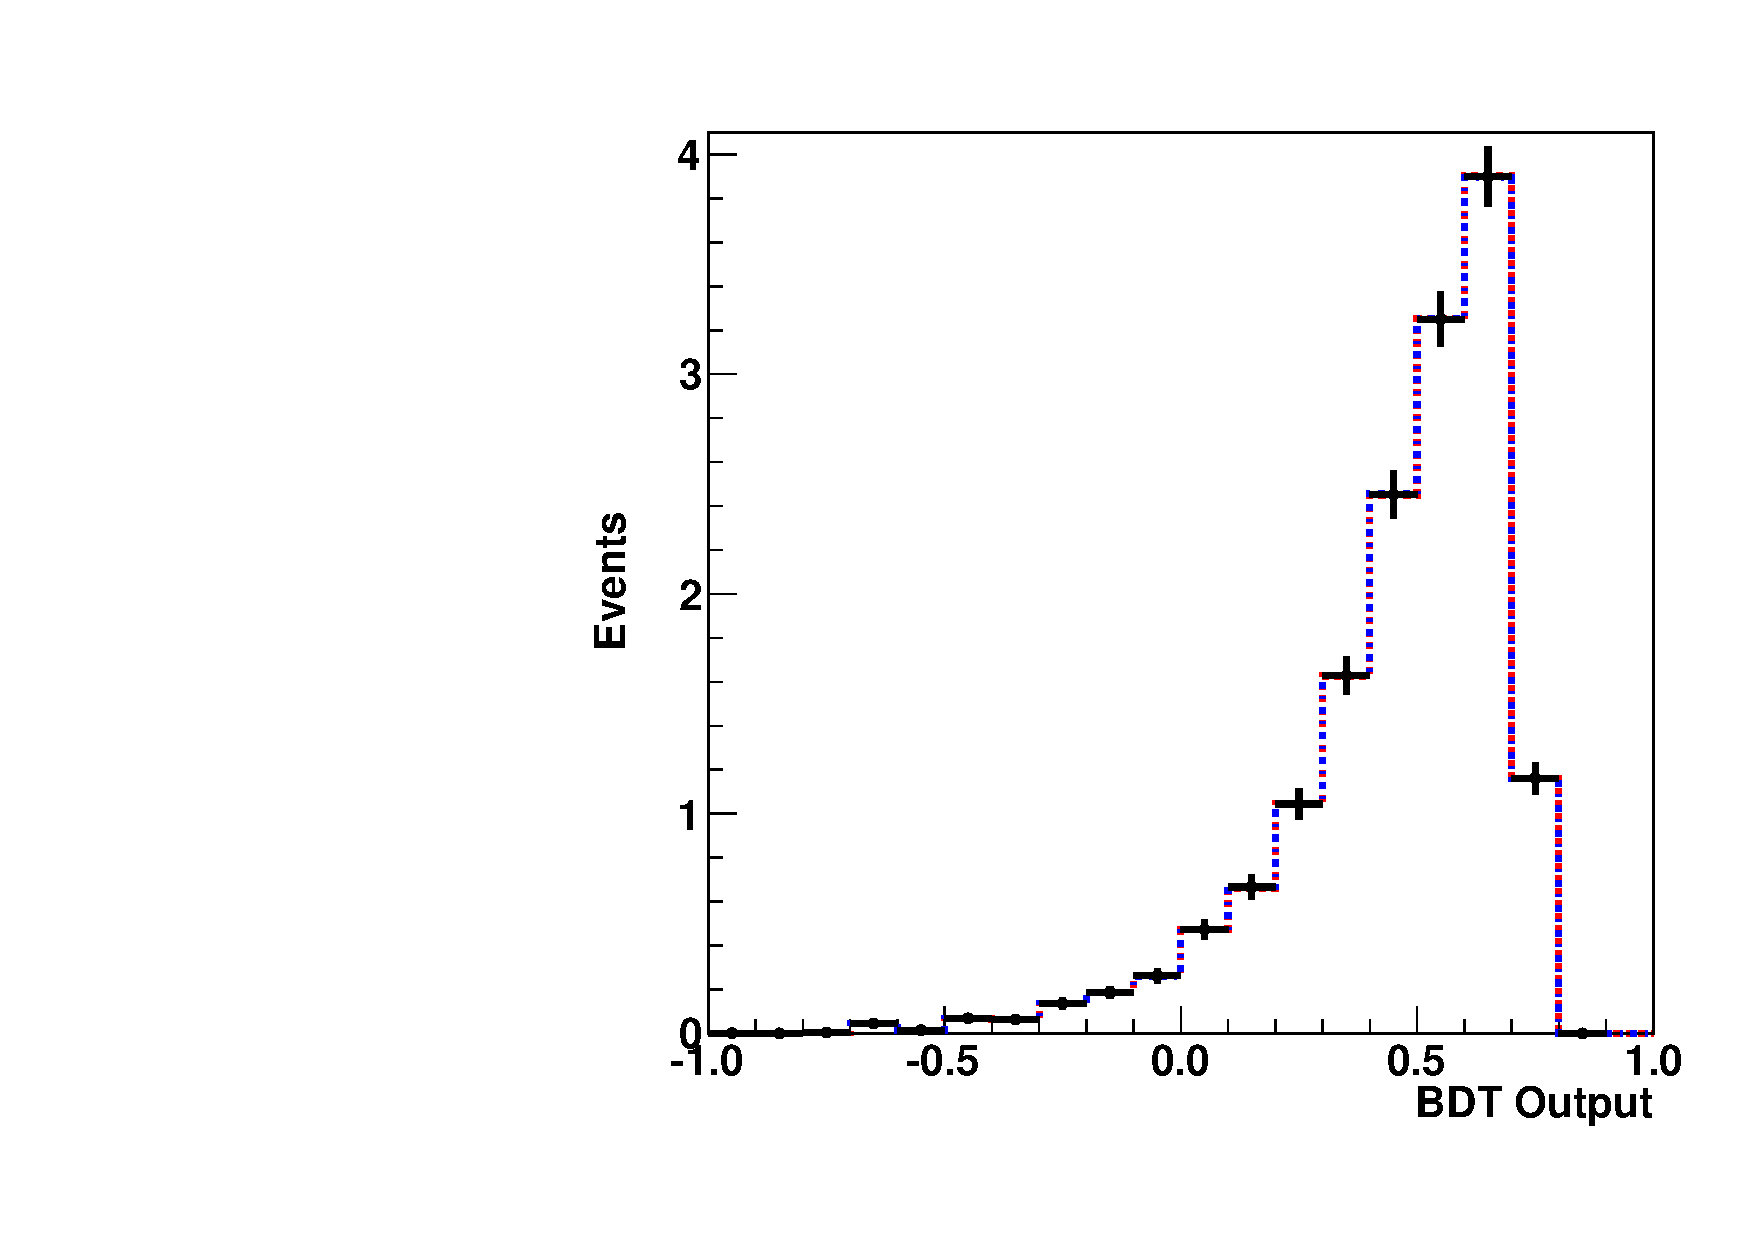
\includegraphics[width=0.49\textwidth]{figures/cvswwsf_58.pdf}}
\caption{BDT Output distribution for $H(130) \to \WW$ 0-jet bin analysis in $gg \to H$ events 
for $\mathcal{L}~=~1.55~\pm~0.07~\ifb$. Opposite-flavor (a) and same-flavor (b) final states 
are shown. The dots histogram is the default shape, while the dashed red histogram 
is the ``Up" component and the dashed blue histograms is the ``Down" component, for the 
theoretical uncertainties.}
\label{fig:ggHsyst}
\end{center}
\end{figure}

\subsubsection{Parton Distribution Functions}
Parton distribution functions (PDFs) are obtained from global fits 
to experimental data from deep in-elastic scattering, Drell-Yan, and jet 
processes. The recommendations of the PDF4LHC group were followed to obtain the
uncertainties due to the limited knowledge of such PDFs. From those studies~\cite{hww_eps, hww_lp}, 
we consider the overall normalisation uncertainty to adequately contain possible 
variations in the uncertainty as a function of the discriminant variable.

\subsubsection{Lepton Efficiency Scale Factors}
The lepton efficiencies are measured in data and simulated events using the 
well-known tag and probe method~\cite{hww_eps}, giving a scale factor to the
simulated events as a function of the $\pt$ and $\eta$ of each lepton. The
associated uncertainty may have some $\pt$ and $\eta$ dependence, leading to a
possible shape variation. The procedure to estimate the uncertainty due to the
lepton efficiency scale factor is to apply a $+1(-1)\sigma$ reweighting factor to the
lepton efficiency scale factor for the ``up" (``down") variation. Both
normalization and shape are considered with this procedure. 
An example of the effect of this uncertainty is shown in Figure~\ref{fig:qqWWeff}. 
It is possible to see that the differences among the default distribution and the 
variations are rather small.

\begin{figure}[!htbp]
\begin{center}
\subfigure[]{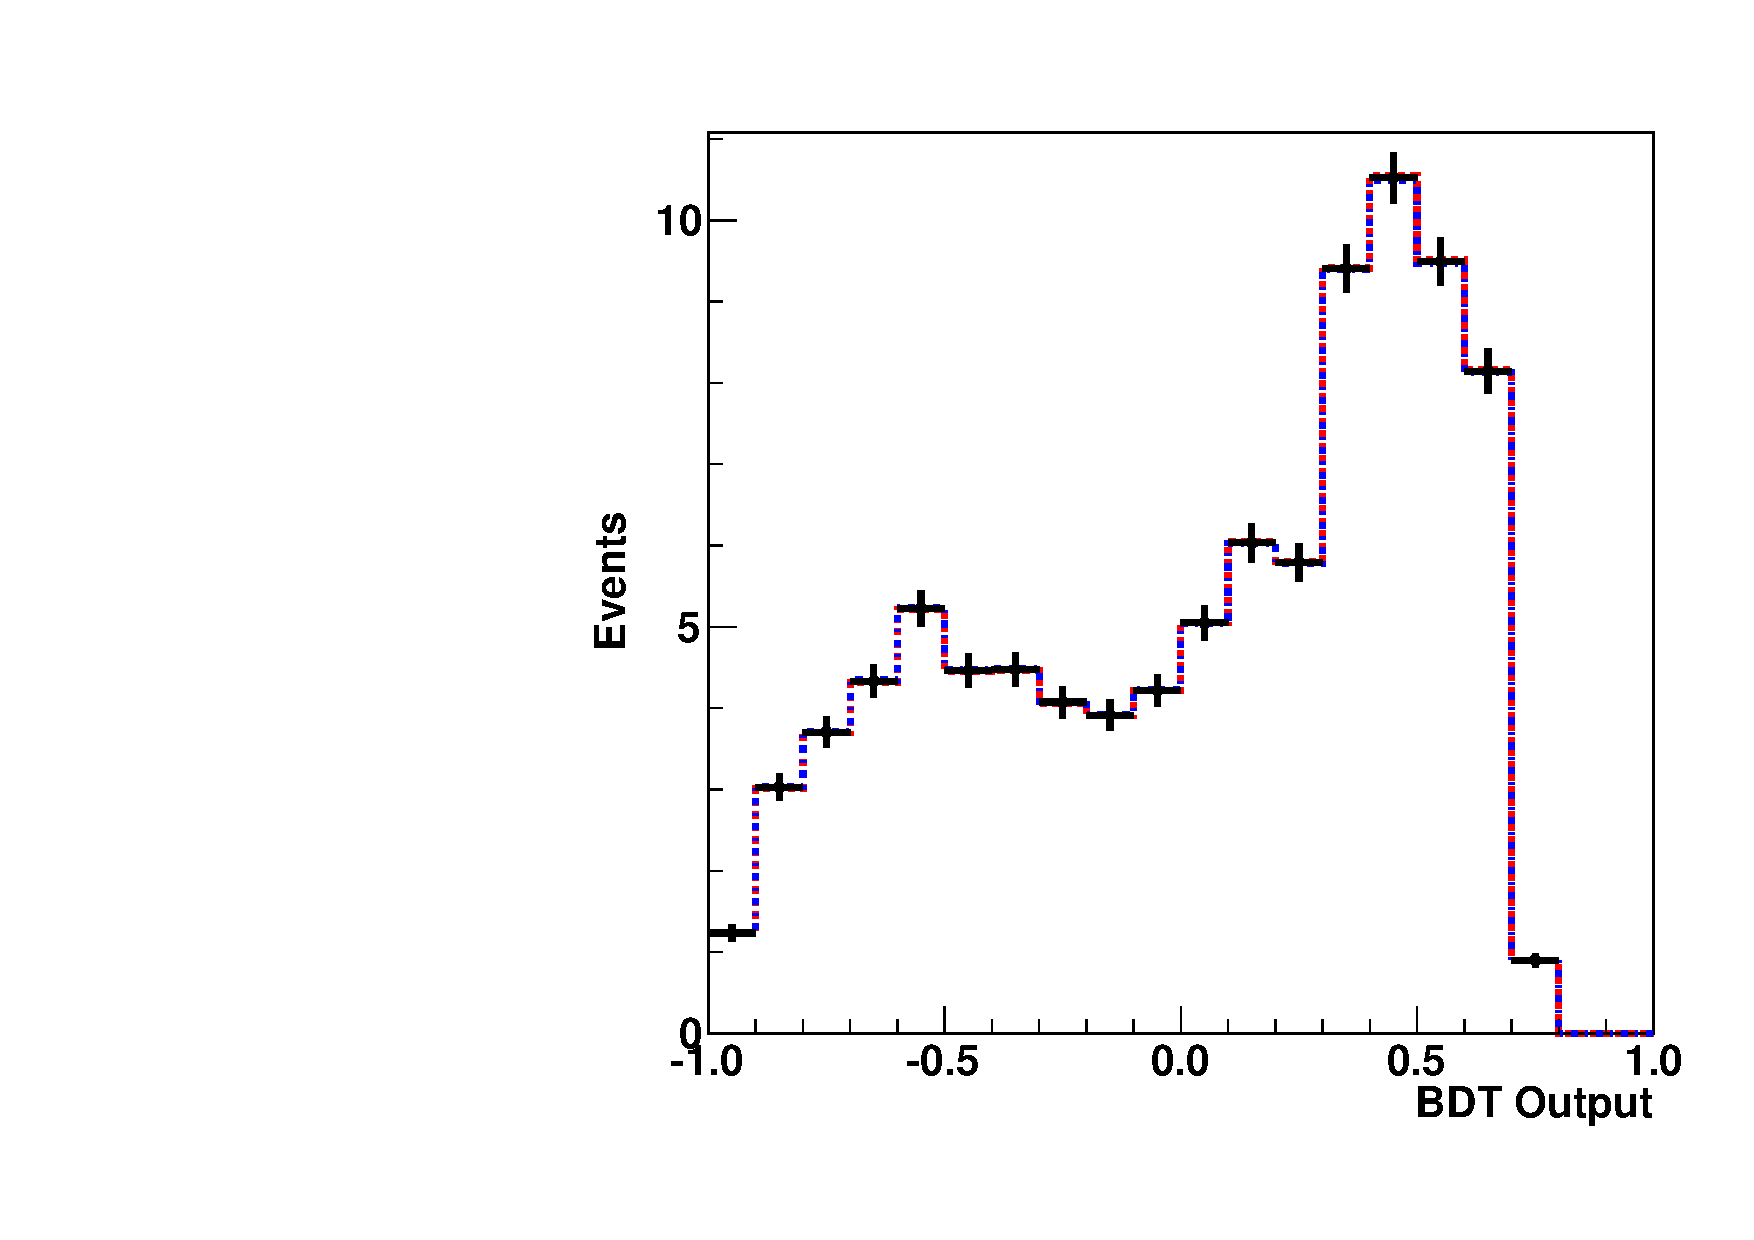
\includegraphics[width=0.49\textwidth]{figures/cvswwof_20.pdf}}
\subfigure[]{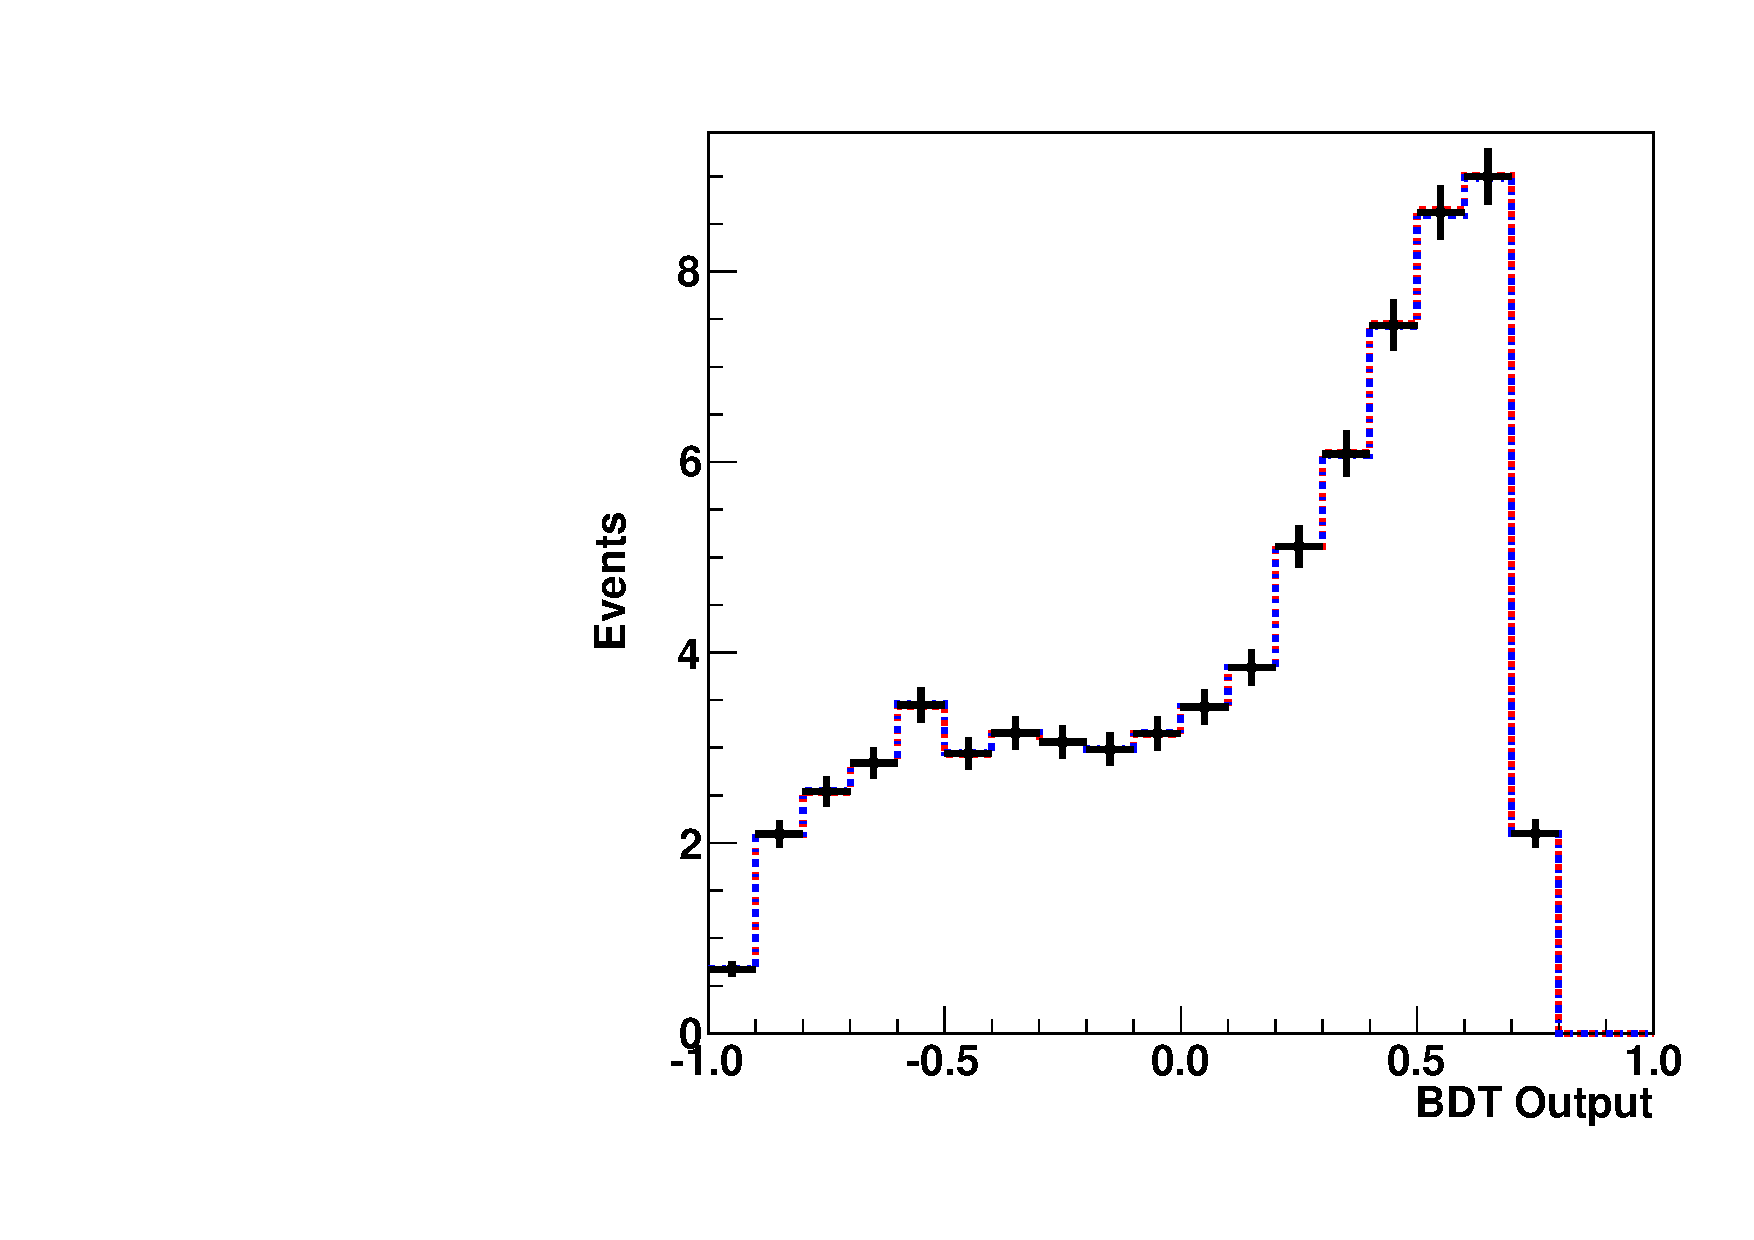
\includegraphics[width=0.49\textwidth]{figures/cvswwsf_20.pdf}}
\caption{BDT Output distribution for $H(130) \to \WW$ 0-jet bin analysis in $qq \to \WW$ events 
for $\mathcal{L}~=~1.55~\pm~0.07~\ifb$. Opposite-flavor (a) and same-flavor (b) final states 
are shown. The dots histogram is the default shape, while the dashed red histogram 
is the ``Up" component and the dashed blue histograms is the ``Down" component, for the 
lepton efficiency uncertainties.}
\label{fig:qqWWeff}
\end{center}
\end{figure}

\subsubsection{Lepton Energy-Momentum Resolution and Scale}
The lepton energy-momentum does not perfectly agree between data and simulated
events with the current available sample. To assign an uncertainty, we smear 
the lepton energy-momentum by a Gaussian with width equal to the central value 
determination of the resolution, and the central value the observed bias in
data. With the new four-momentum of both leptons, we build a new discriminant
variable. We take the ``up" (``down") variation as the positive (negative) biased
case. 
An example of the effect of this uncertainty is shown in Figure~\ref{fig:ggWWLepRes}. 

\begin{figure}[!htbp]
\begin{center}
\subfigure[]{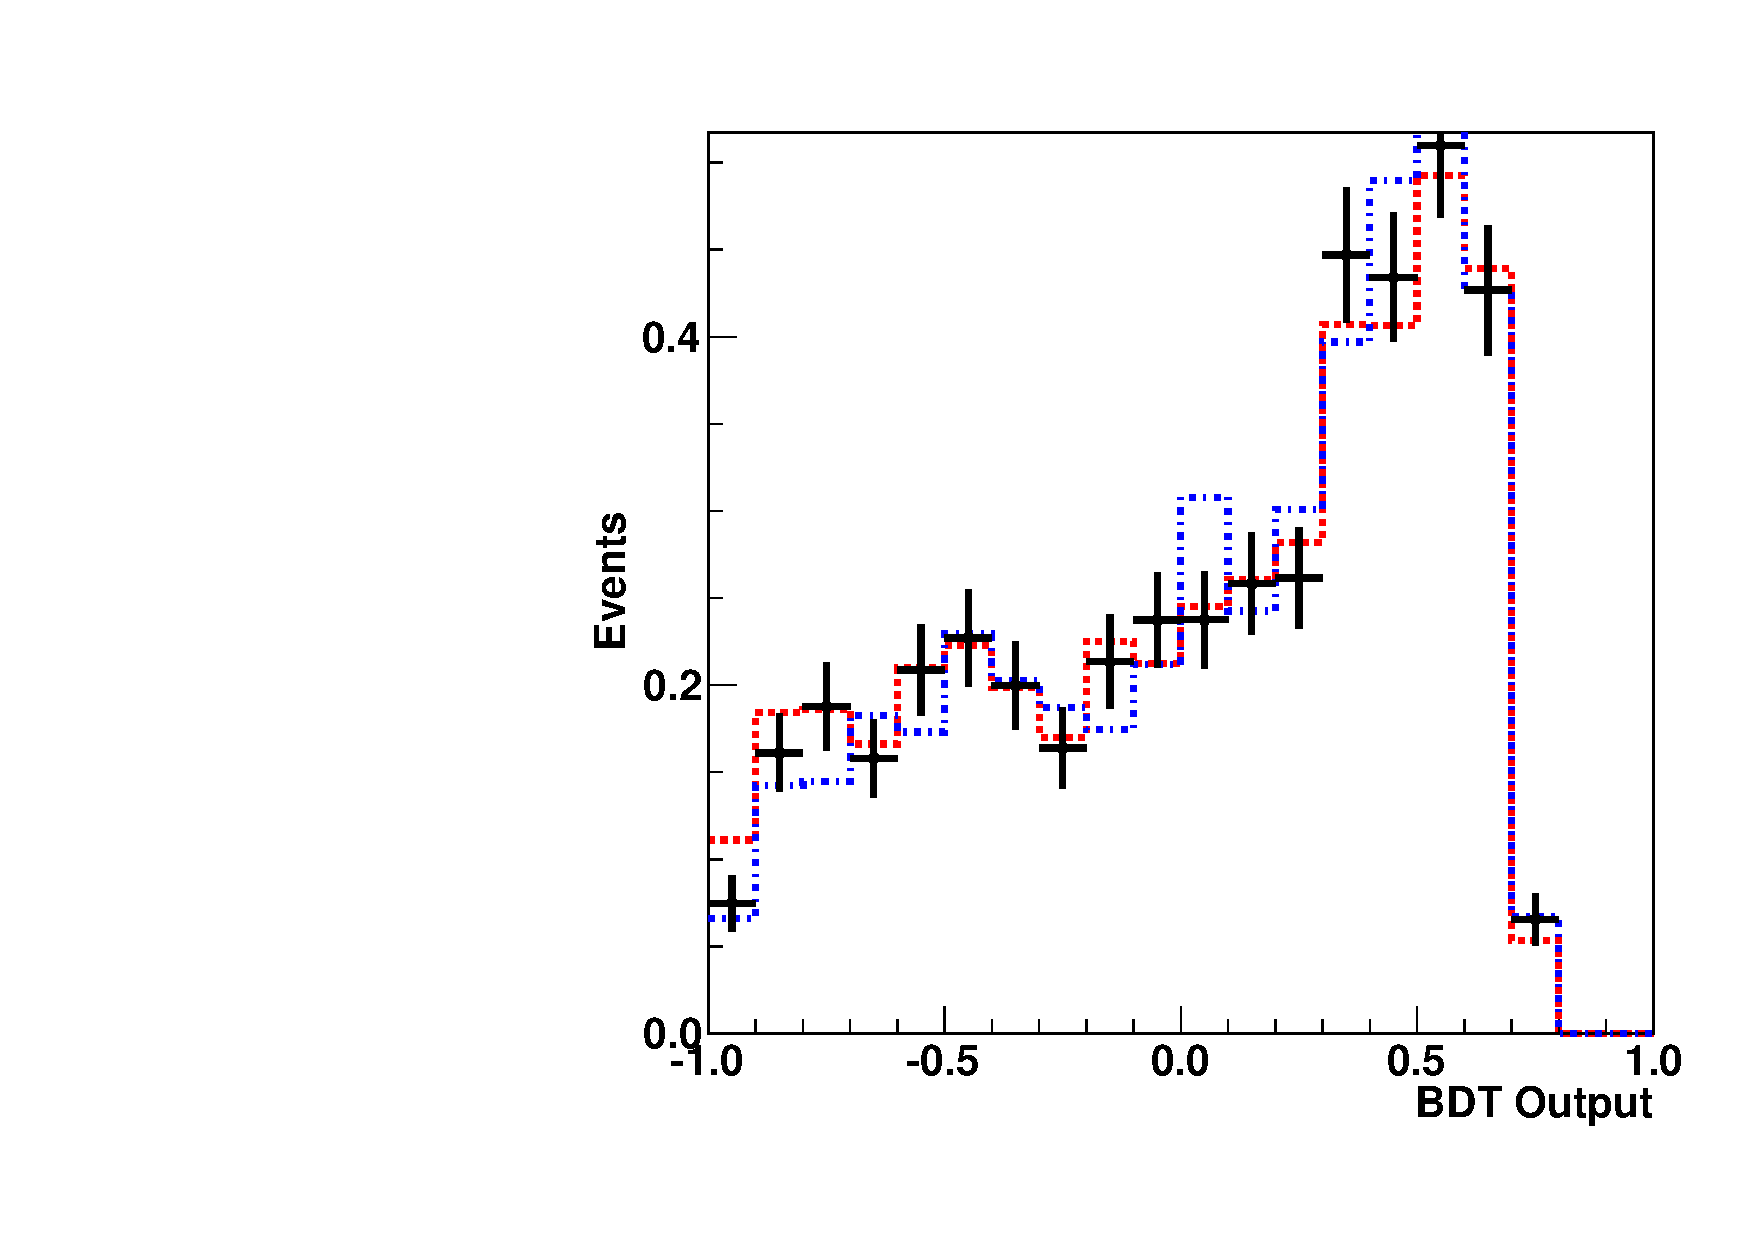
\includegraphics[width=0.49\textwidth]{figures/cvswwof_31.pdf}}
\subfigure[]{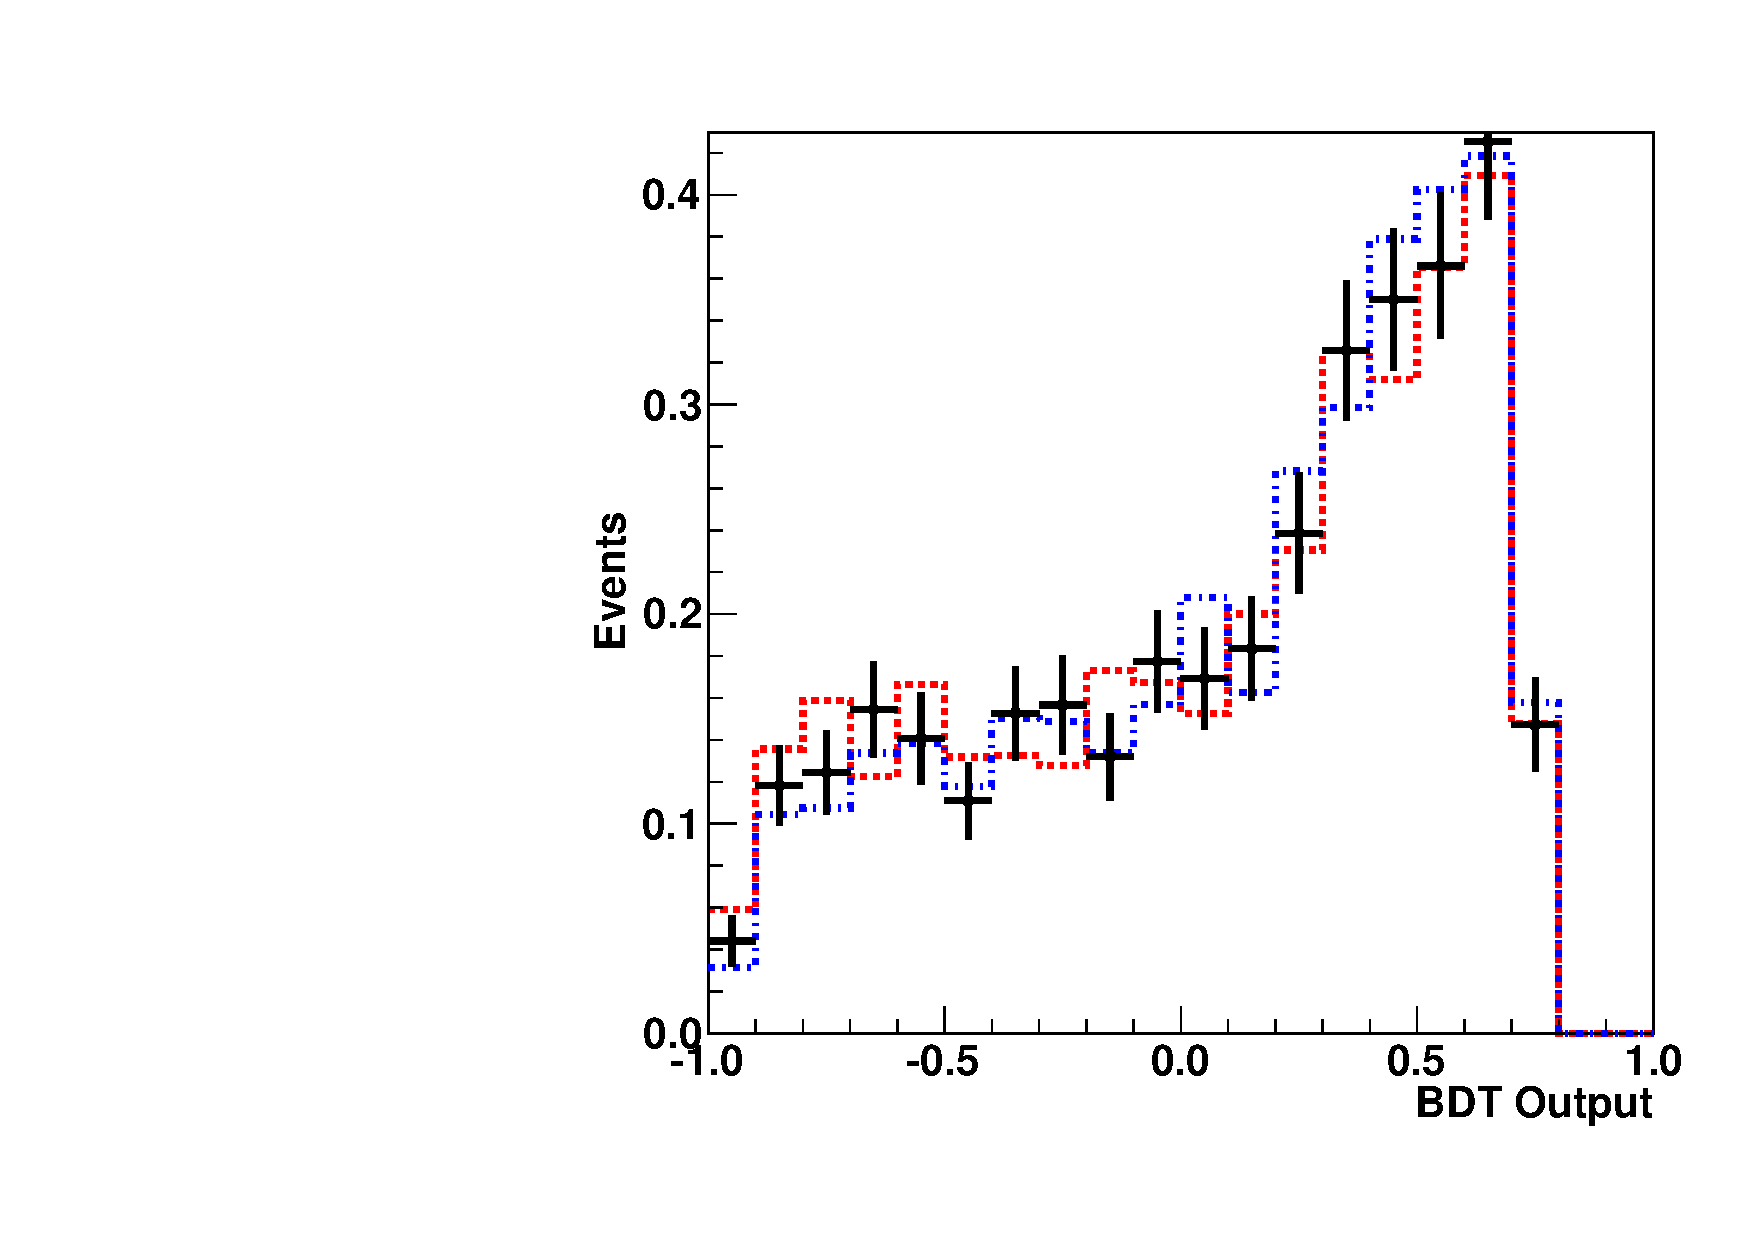
\includegraphics[width=0.49\textwidth]{figures/cvswwsf_31.pdf}}
\caption{BDT Output distribution for $H(130) \to \WW$ 0-jet bin analysis in $gg \to \WW$ events 
for $\mathcal{L}~=~1.55~\pm~0.07~\ifb$. Opposite-flavor (a) and same-flavor (b) final states 
are shown. The dots histogram is the default shape, while the dashed red histogram 
is the ``Up" component and the dashed blue histograms is the ``Down" component, for the 
lepton momentum resolution and scale uncertainties.}
\label{fig:ggWWLepRes}
\end{center}
\end{figure}

\subsubsection{$\met$ Resolution}
The $\met$ resolution in data is not well reproduced in simulated events leading
to an underestimation of $\dyll$ events, where no real $\met$ from neutrinos is
present. The background estimation from Zjets events has its own uncertainty.
Nevertheless, other processes with neutrinos in the final state may have an
uncertainty due to this effect. To account for it, we have smeared the X and Y
components of both $\met$ and $track-\met$ and produced new discriminant
variables with the smeared quantities. The smeared variable is the ``up"
variation, while we take the ``down" variation as the mirror of the difference
between the ``up" and default variables. 
An example of the effect of this uncertainty is shown in Figure~\ref{fig:VVMetRes}. 

\begin{figure}[!htbp]
\begin{center}
\subfigure[]{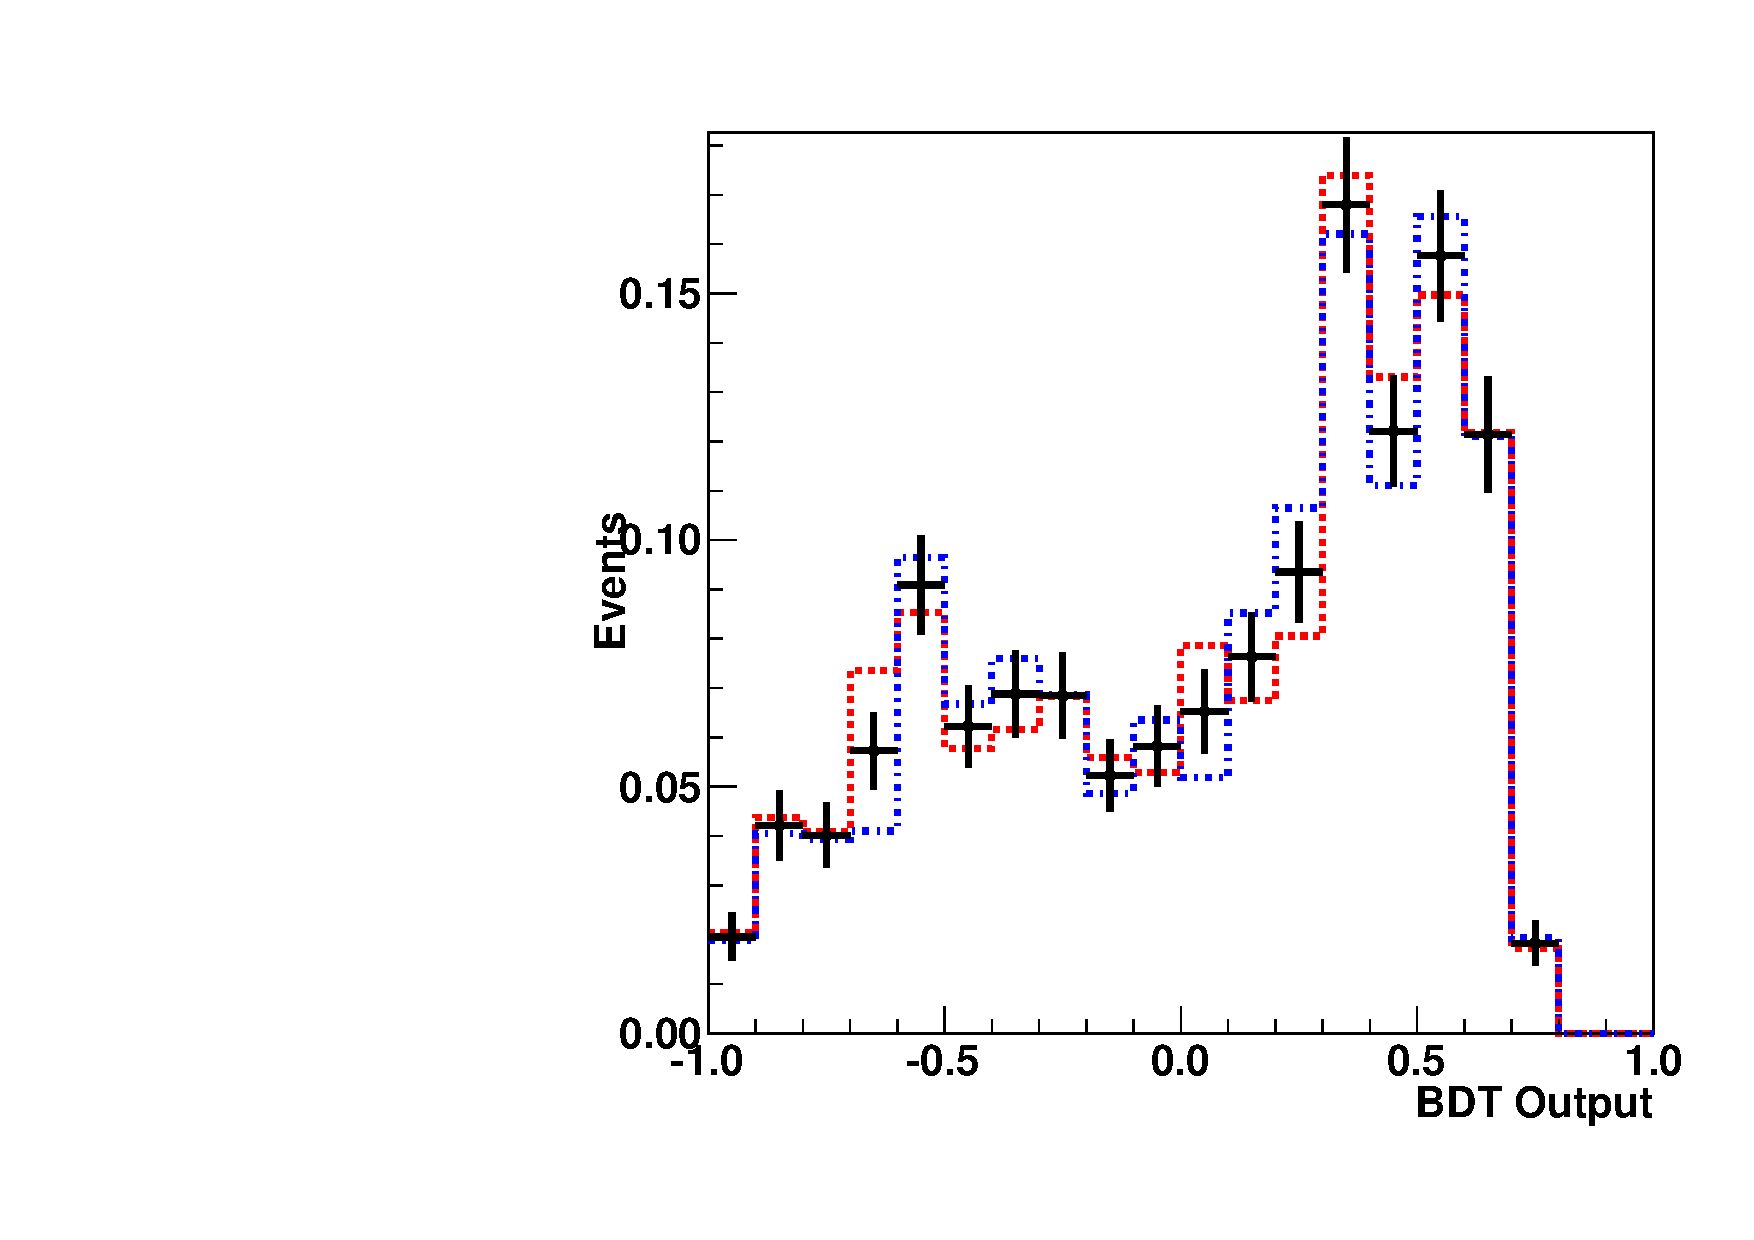
\includegraphics[width=0.49\textwidth]{figures/cvswwof_43.pdf}}
\subfigure[]{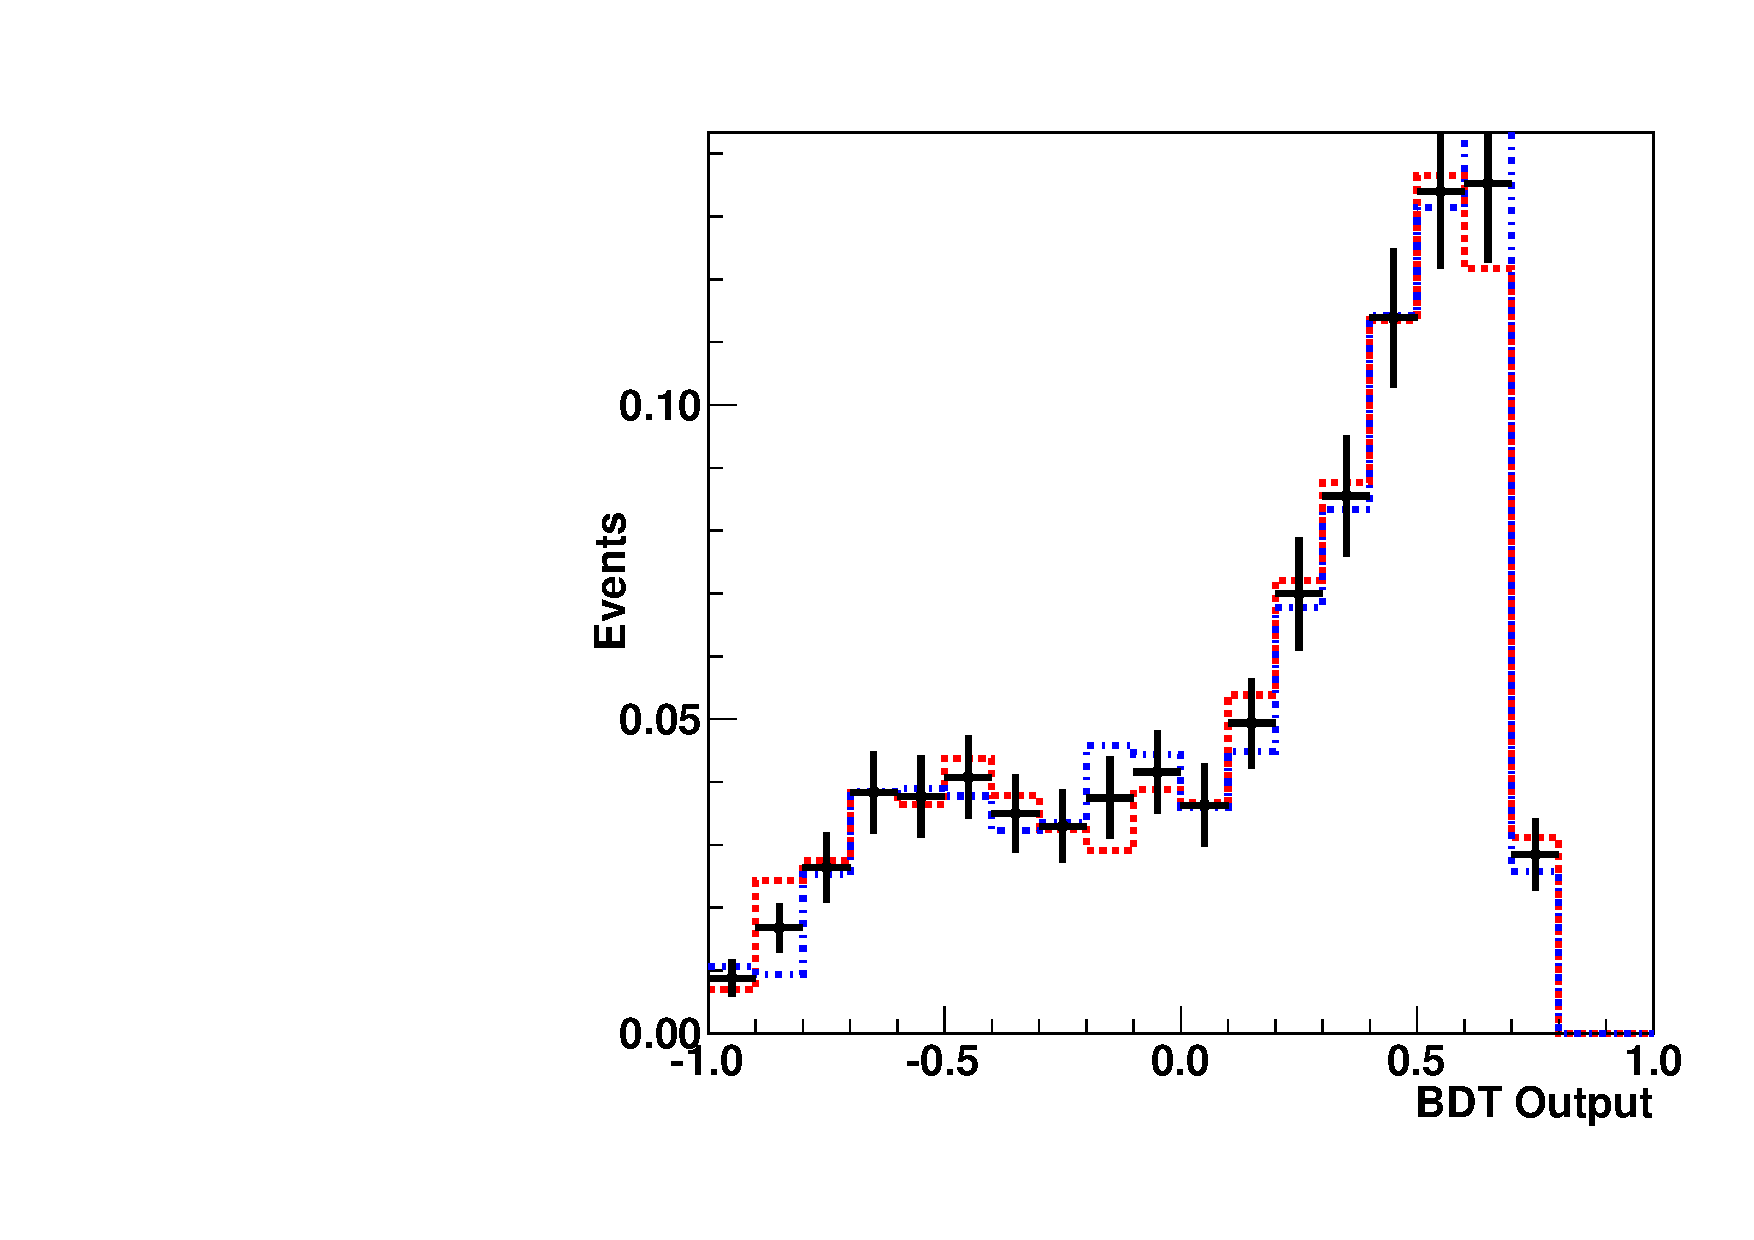
\includegraphics[width=0.49\textwidth]{figures/cvswwsf_43.pdf}}
\caption{BDT Output distribution for $H(130) \to \WW$ 0-jet bin analysis in $\WZ/\Z\Z$ events 
for $\mathcal{L}~=~1.55~\pm~0.07~\ifb$. Opposite-flavor (a) and same-flavor (b) final states 
are shown. The dots histogram is the default shape, while the dashed red histogram 
is the ``Up" component and the dashed blue histograms is the ``Down" component, for the 
$\met$ uncertainties.}
\label{fig:VVMetRes}
\end{center}
\end{figure}

\subsubsection{Jet Energy Scale}
The discriminant variables make no use of the jet energy quantities, therefore
there is no direct effect on the jet energy scale (JES) uncertainty, in addition
to the normalization uncertainty due to the migration among the different jet
bins. Nevertheless, it is observed that kinematic variables show different
distributions depending on the jet multiplicity. To assign an uncertainty,
we vary the transverse momentum of the jets by $\pm 5\%$ (``up" and ``down",
respectively) and build the new discriminant variables. Only shape uncertainties are 
considered in this case. 
An example of the effect of this uncertainty is shown in Figure~\ref{fig:ggHJES}. 
It is possible to see that the differences among the default distribution and the 
variations are rather small.

\begin{figure}[!htbp]
\begin{center}
\subfigure[]{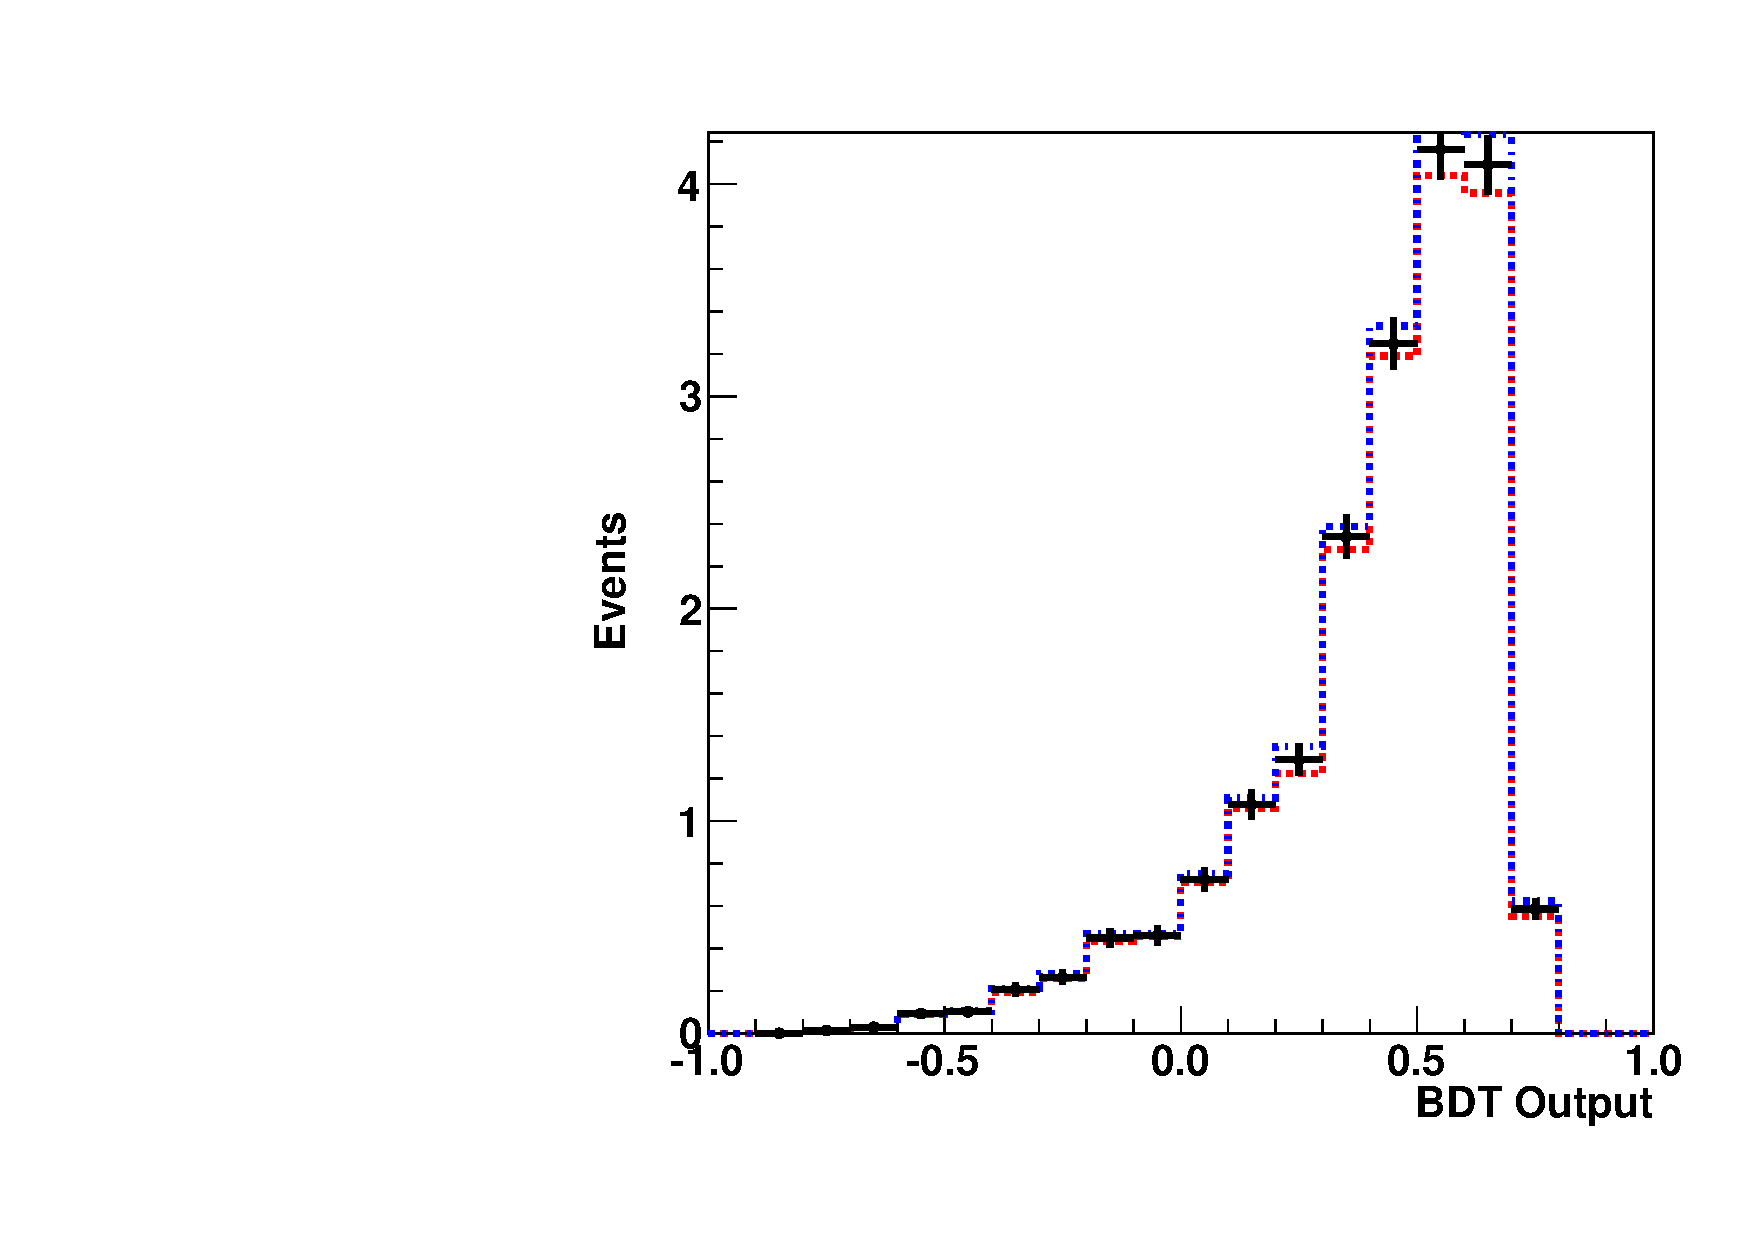
\includegraphics[width=0.49\textwidth]{figures/cvswwof_50.pdf}}
\subfigure[]{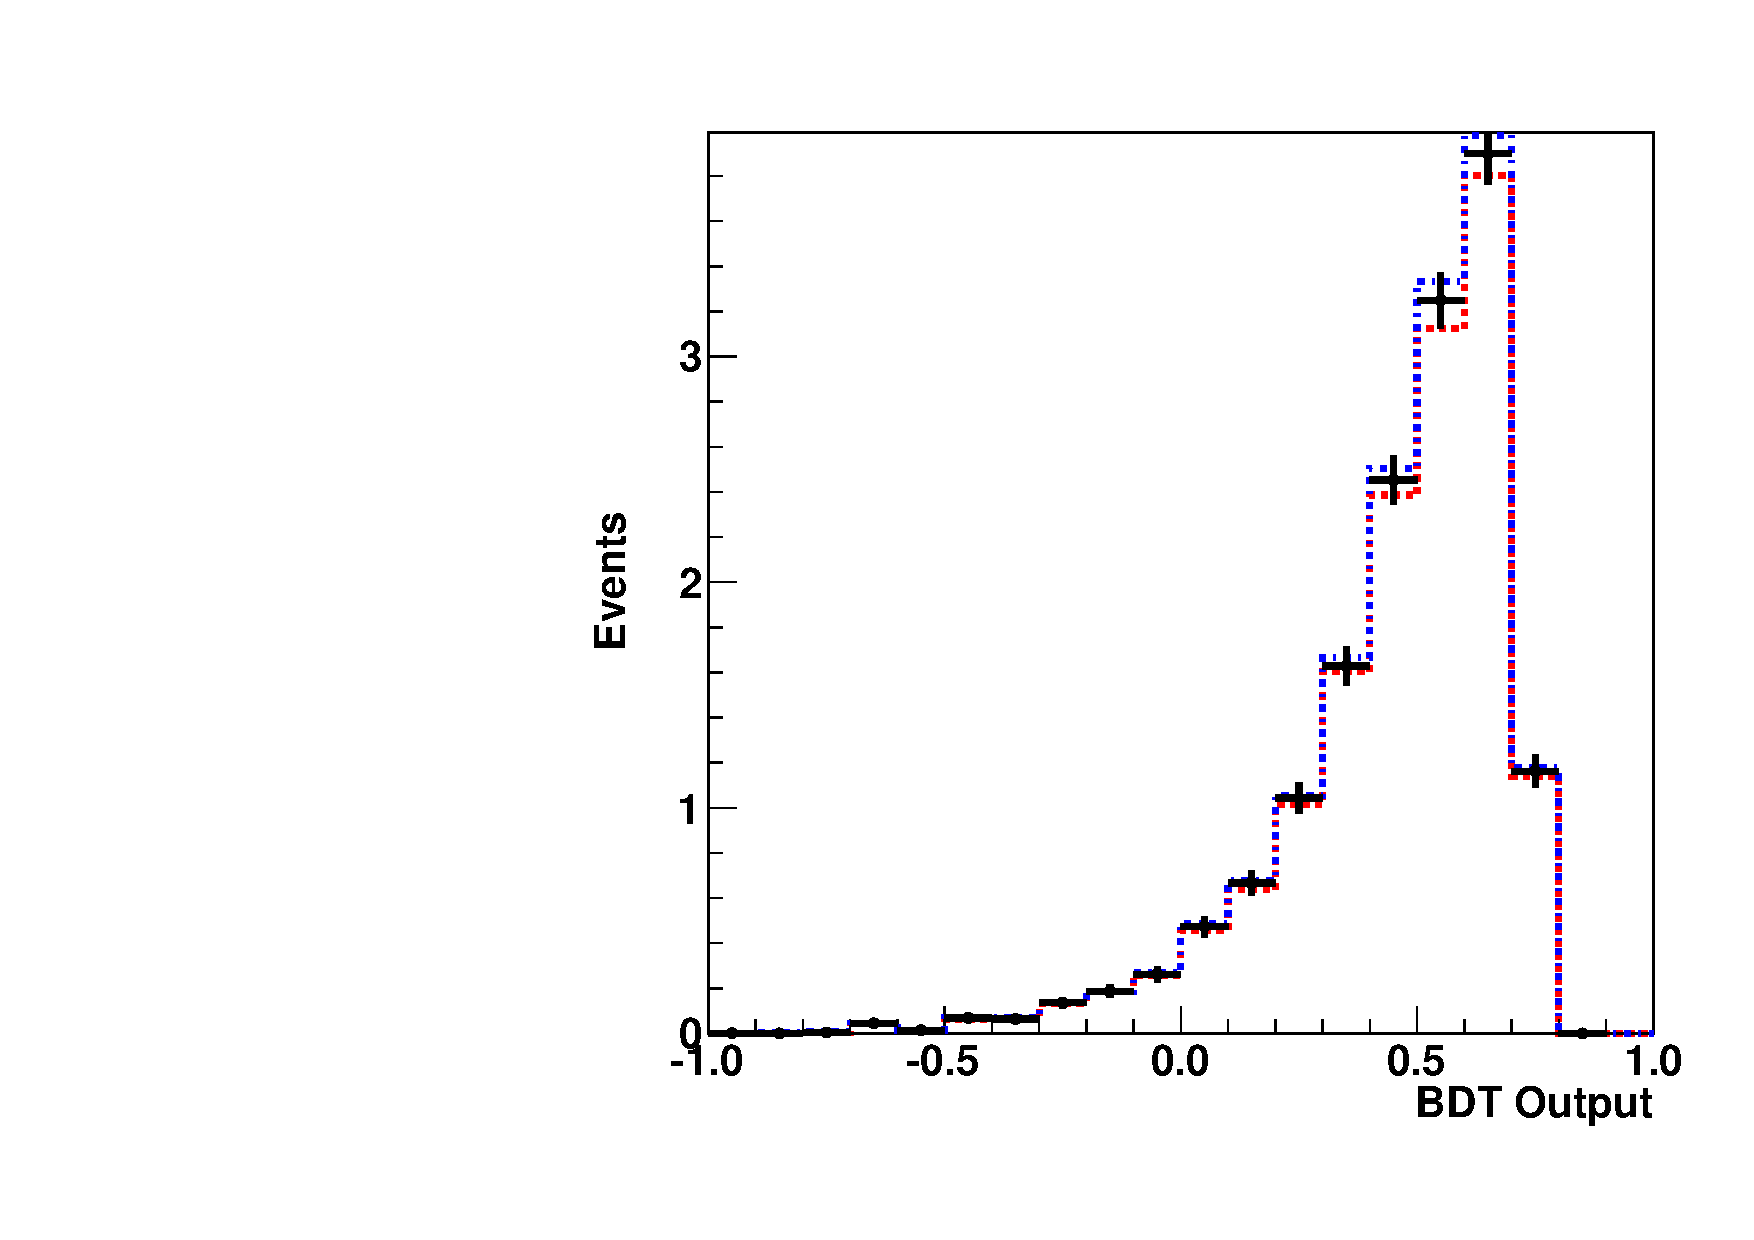
\includegraphics[width=0.49\textwidth]{figures/cvswwsf_50.pdf}}
\caption{BDT Output distribution for $H(130) \to \WW$ 0-jet bin analysis in $gg \to H$ events 
for $\mathcal{L}~=~1.55~\pm~0.07~\ifb$. Opposite-flavor (a) and same-flavor (b) final states 
are shown. The dots histogram is the default shape, while the dashed red histogram 
is the ``Up" component and the dashed blue histograms is the ``Down" component, for the JES 
uncertainties.}
\label{fig:ggHJES}
\end{center}
\end{figure}

\subsubsection{$\WW$ Background}
This effect considers the theoretical uncertainties on the $\WW$ background, in
addition to the normalization uncertainty which has its own factor. The 
$gg \to \WW$ has an uncertainty due to the QCD scales of 50\% and covers very
well any possible shape variation.

To account for possible shape variation on the $qq \to \WW$ process, two 
separate effects are considered. First, we compare the default simulated events
produced with Madgraph generator with simulated events produced with MC@NLO
generator, and this second sample makes the ``up" variation. The ``down"
variation is the mirror of the ratio between both generators. Second, we consider
the uncertainty due to the variation of the QCD scales. To perform that, we take
the ratio between the MC@NLO samples and the ones with the QCD scales up and down. 
An example of the effect of this uncertainty is shown in Figure~\ref{fig:qqWWNorn}. 

\begin{figure}[!htbp]
\begin{center}
\subfigure[]{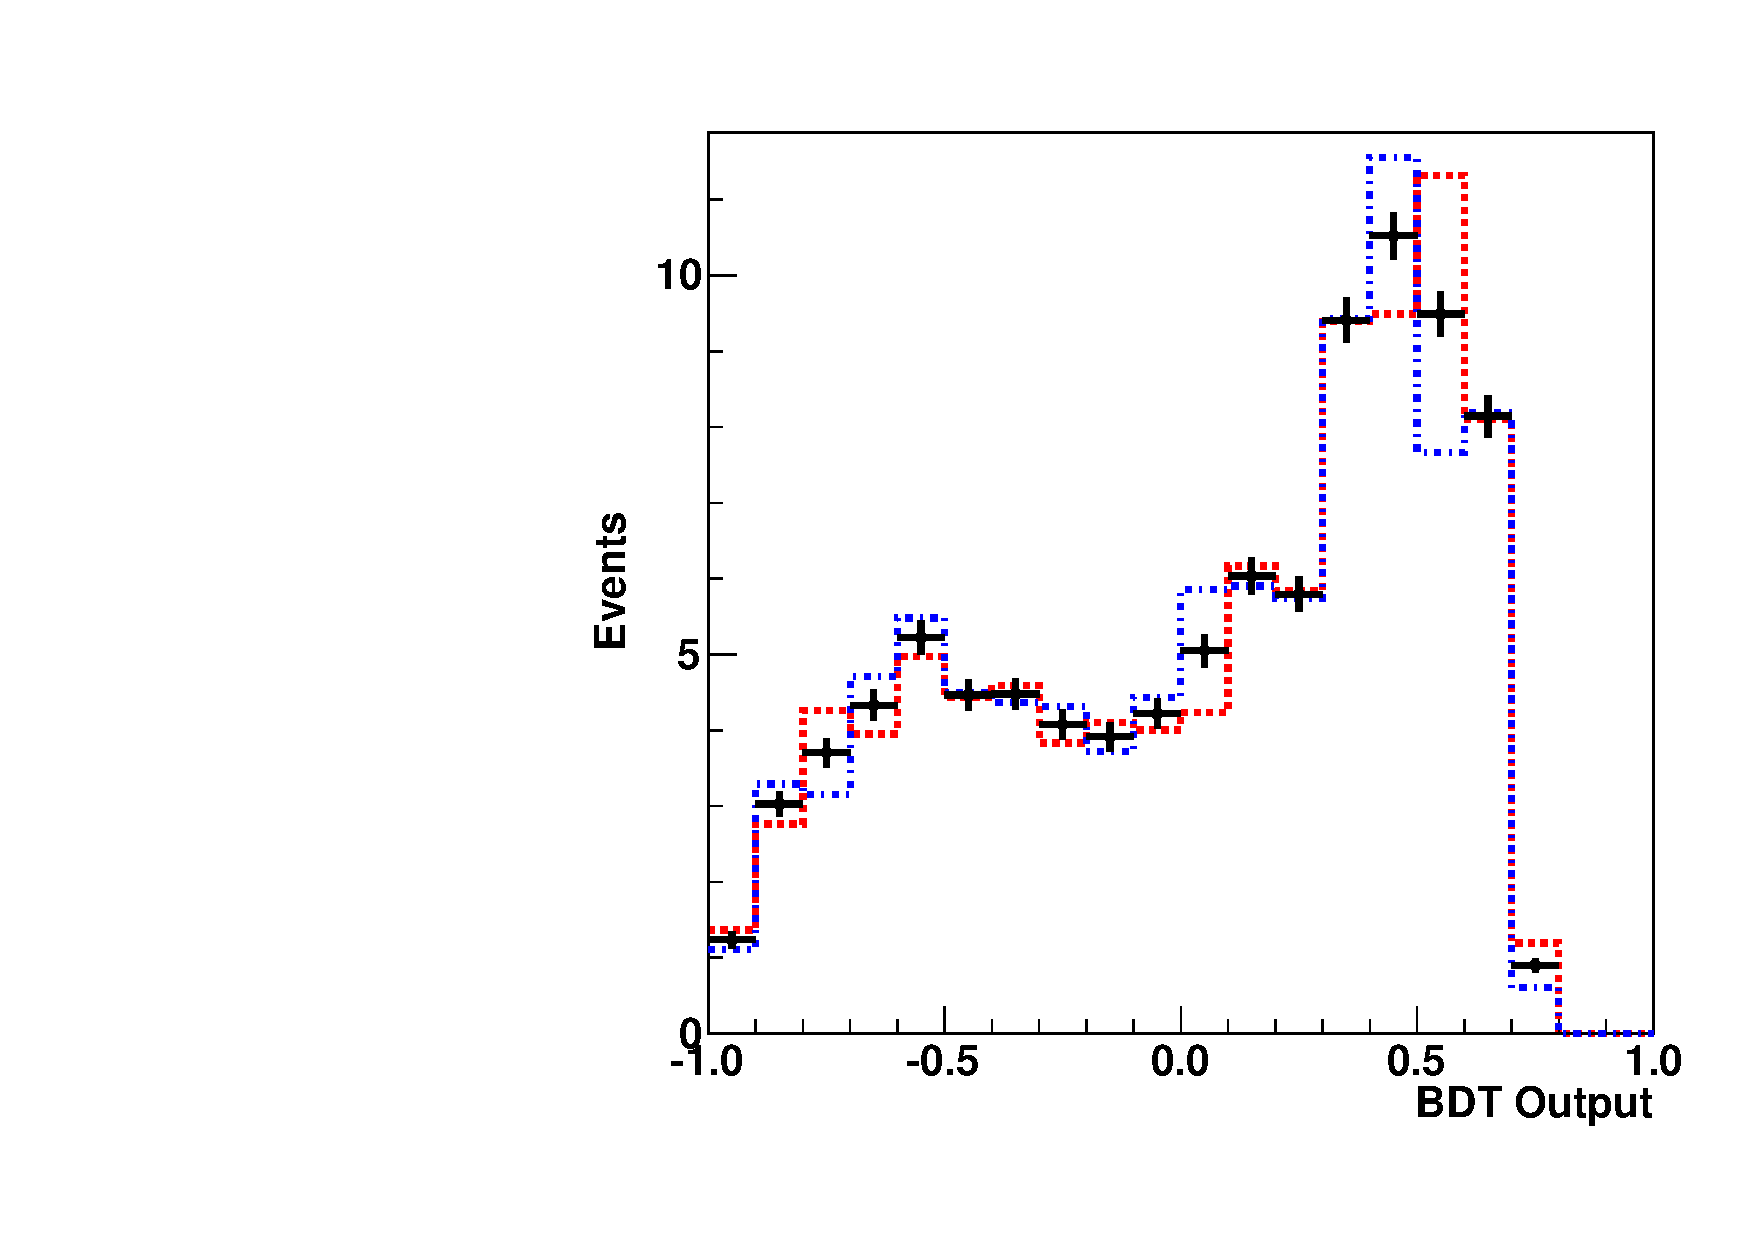
\includegraphics[width=0.49\textwidth]{figures/cvswwof_0.pdf}}
\subfigure[]{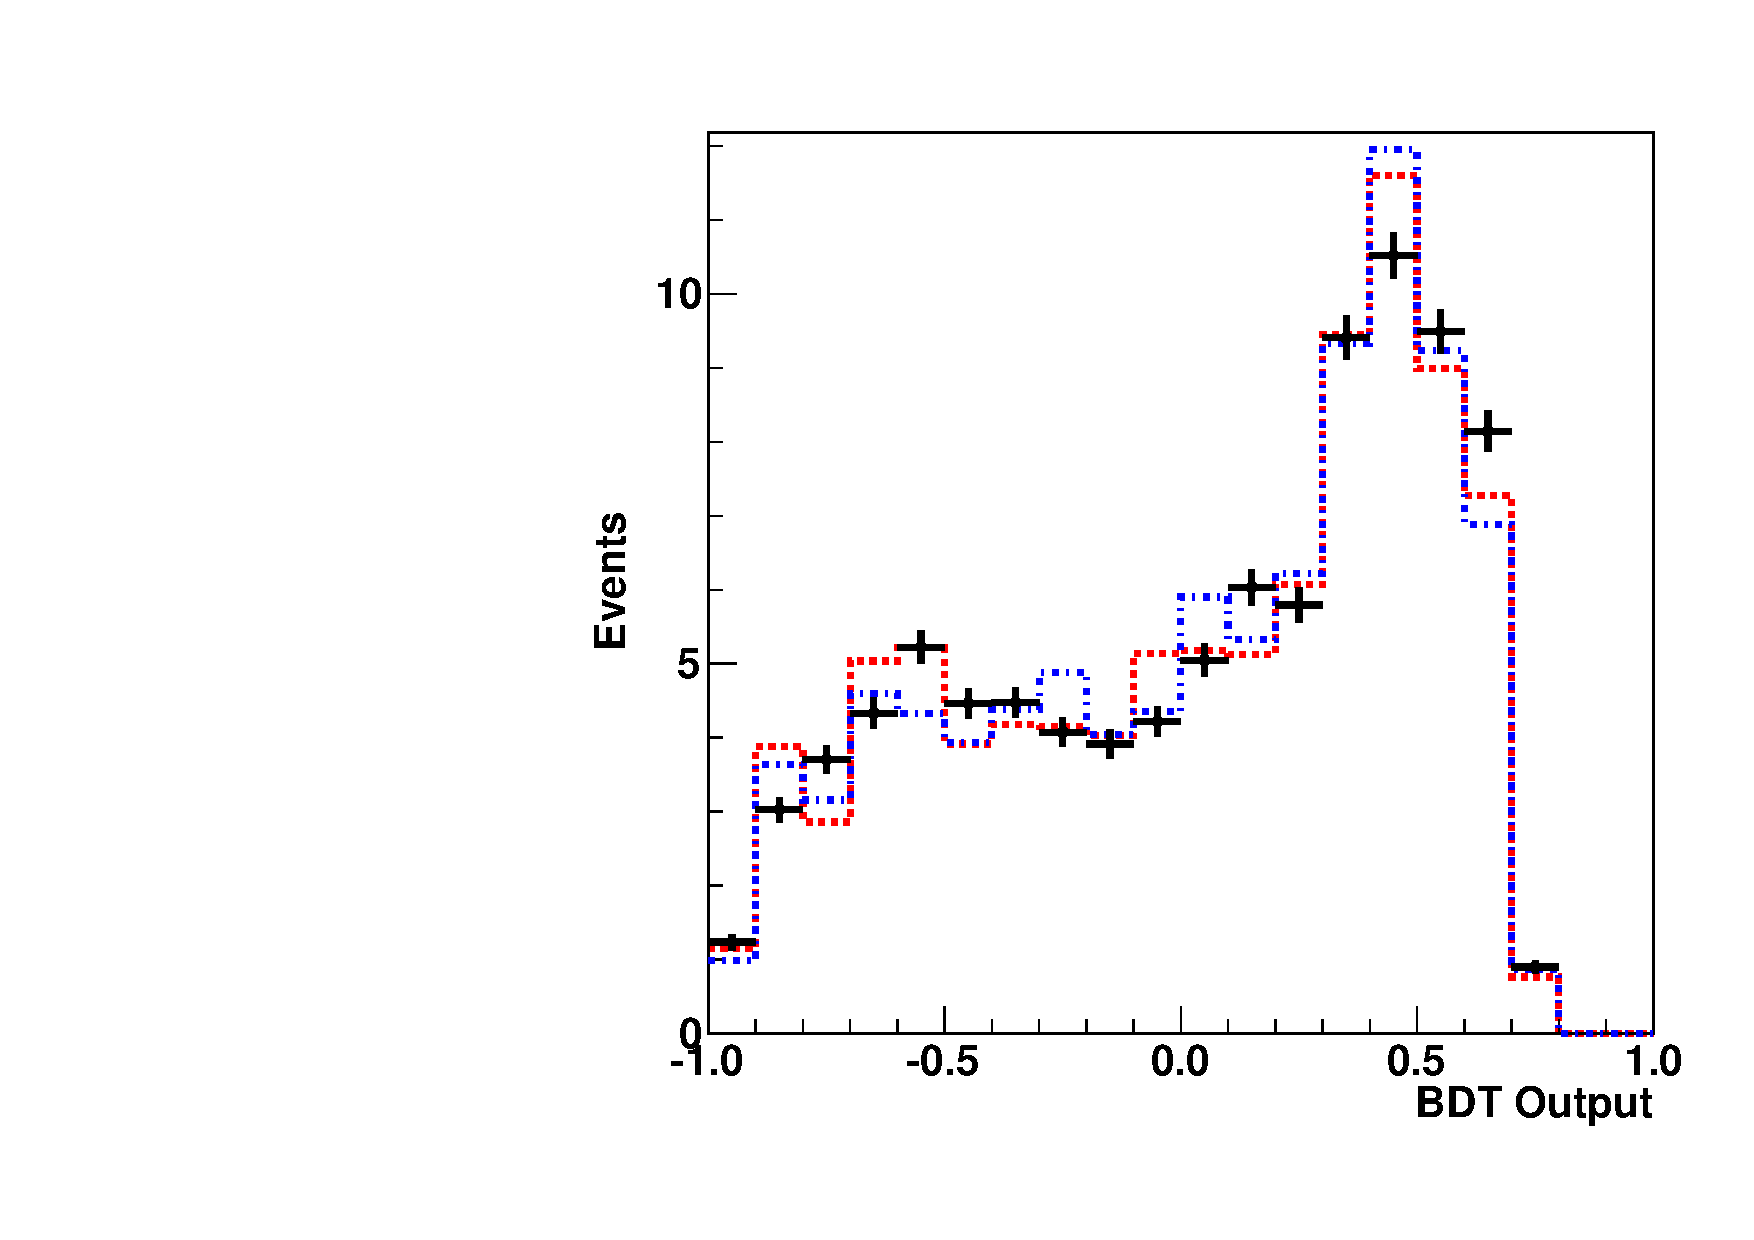
\includegraphics[width=0.49\textwidth]{figures/cvswwof_59.pdf}}
\caption{BDT Output distribution for $H(130) \to \WW$ 0-jet bin analysis opposite-flavor final state in $qq \to \WW$ events 
for $\mathcal{L}~=~1.55~\pm~0.07~\ifb$. The dots histogram is the default shape, while the dashed red histogram 
is the ``Up" component and the dashed blue histograms is the ``Down" component, for the generator 
dependence uncertainty (a) and for the QCD scale uncertainties (b).}
\label{fig:qqWWNorn}
\end{center}
\end{figure}

\subsubsection{$\Wjets$ Background}
The uncertainty due to the $\Wjets$ normalization is as large as $\sim$36\%.
Nevertheless, we may have an additional uncertainty on the shape of the
discriminant variable. Two sources are considered. First, we produce new
distributions by using different lepton fake rates, this is the ``up" variation.
The ``down" variation is the mirror of the ratio between the ``up" and default
distributions. The muon fake rate is built using a jet $\pt$ threshold of 30
$\GeVc$ (instead of 15, the default value), and the electron fake rate is build
using a jet $\pt$ threshold of 50 $\GeVc$ (instead of 35, the default value).
Second, we propagate the Monte Carlo closure test uncertainty. To do that, we use
the lepton plus fakeable object sample from Monte Carlo events and apply 
the measured lepton fake rates to build a new $\Wjets$ distribution. This
produces the ``up" variation. The ``down" variation is the mirror of the ration
between the ``up" and default distributions. 
An example of the effect of this uncertainty is shown in Figure~\ref{fig:WJetsNorn}. 

\begin{figure}[!htbp]
\begin{center}
\subfigure[]{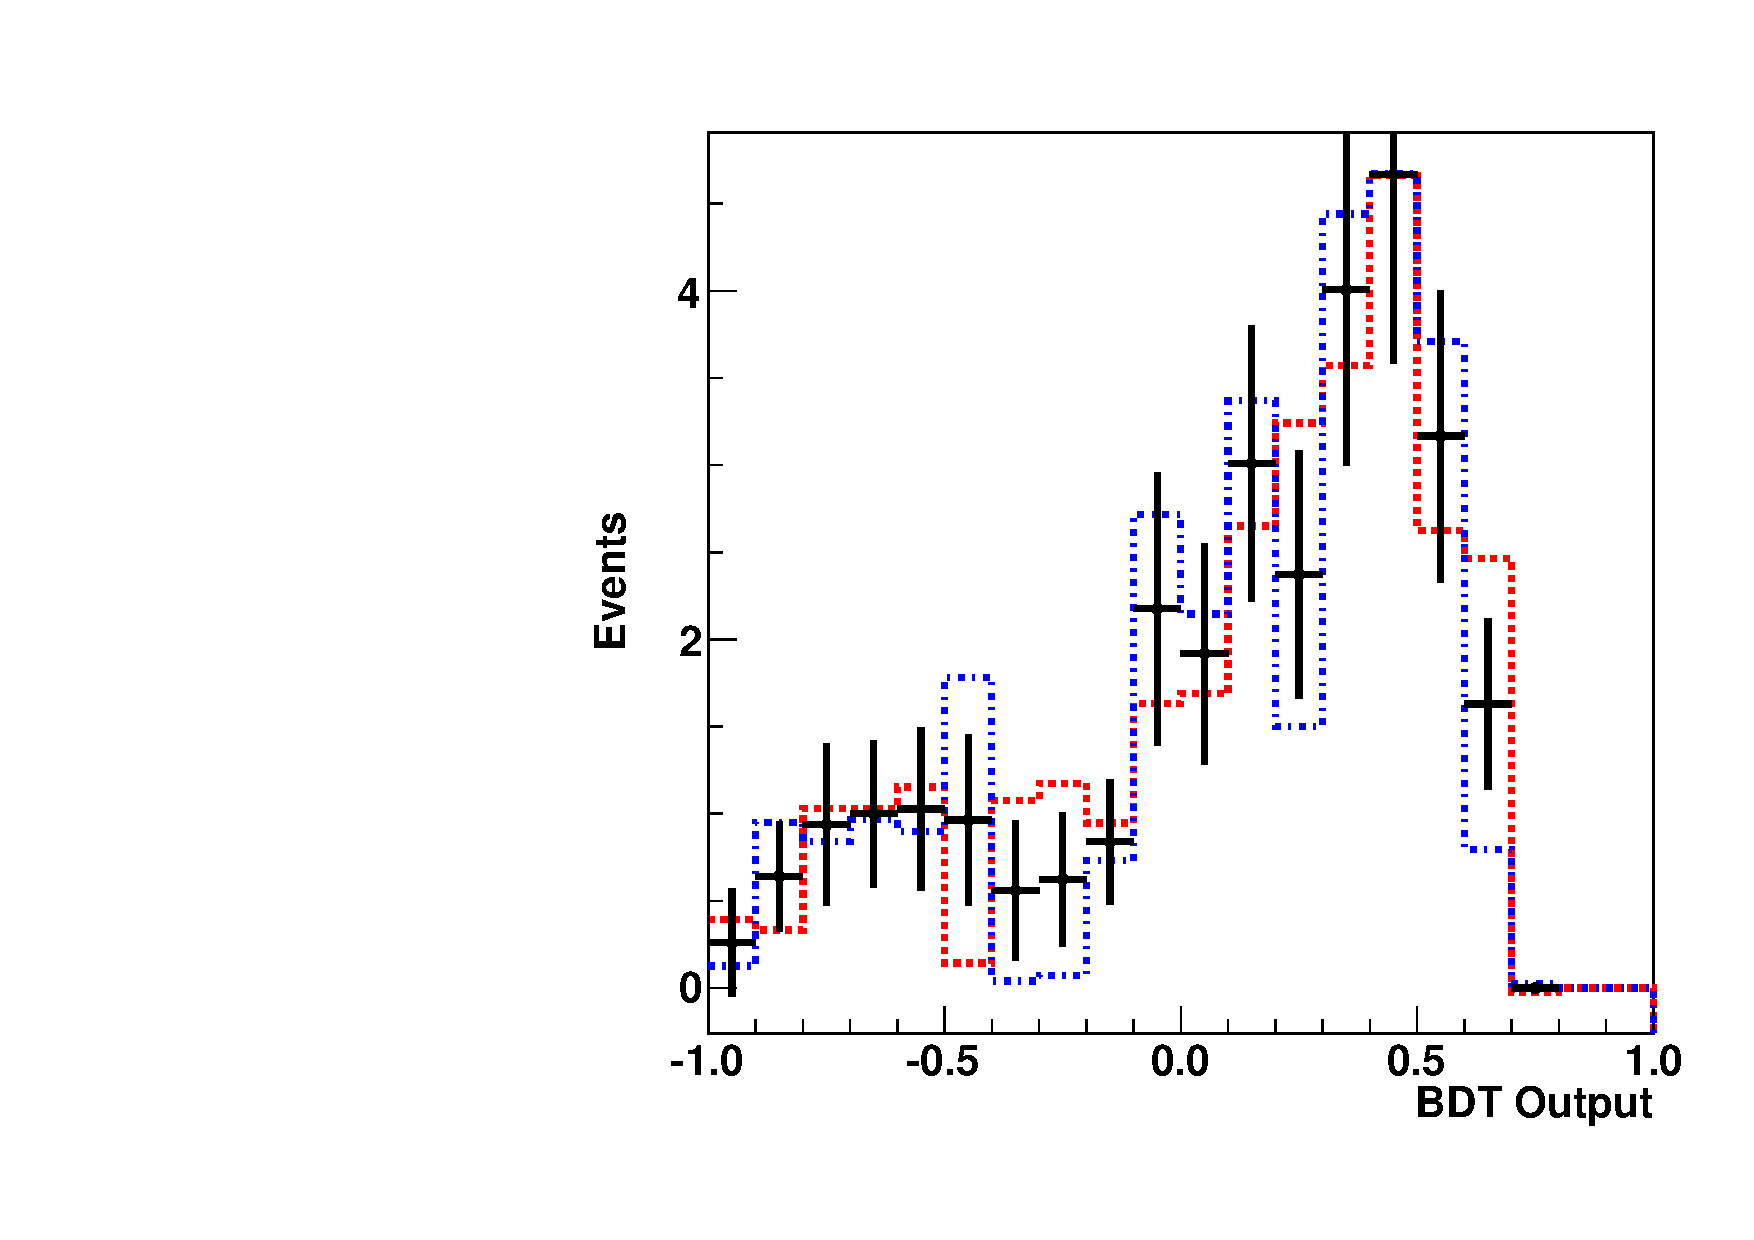
\includegraphics[width=0.49\textwidth]{figures/cvswwof_56.pdf}}
\subfigure[]{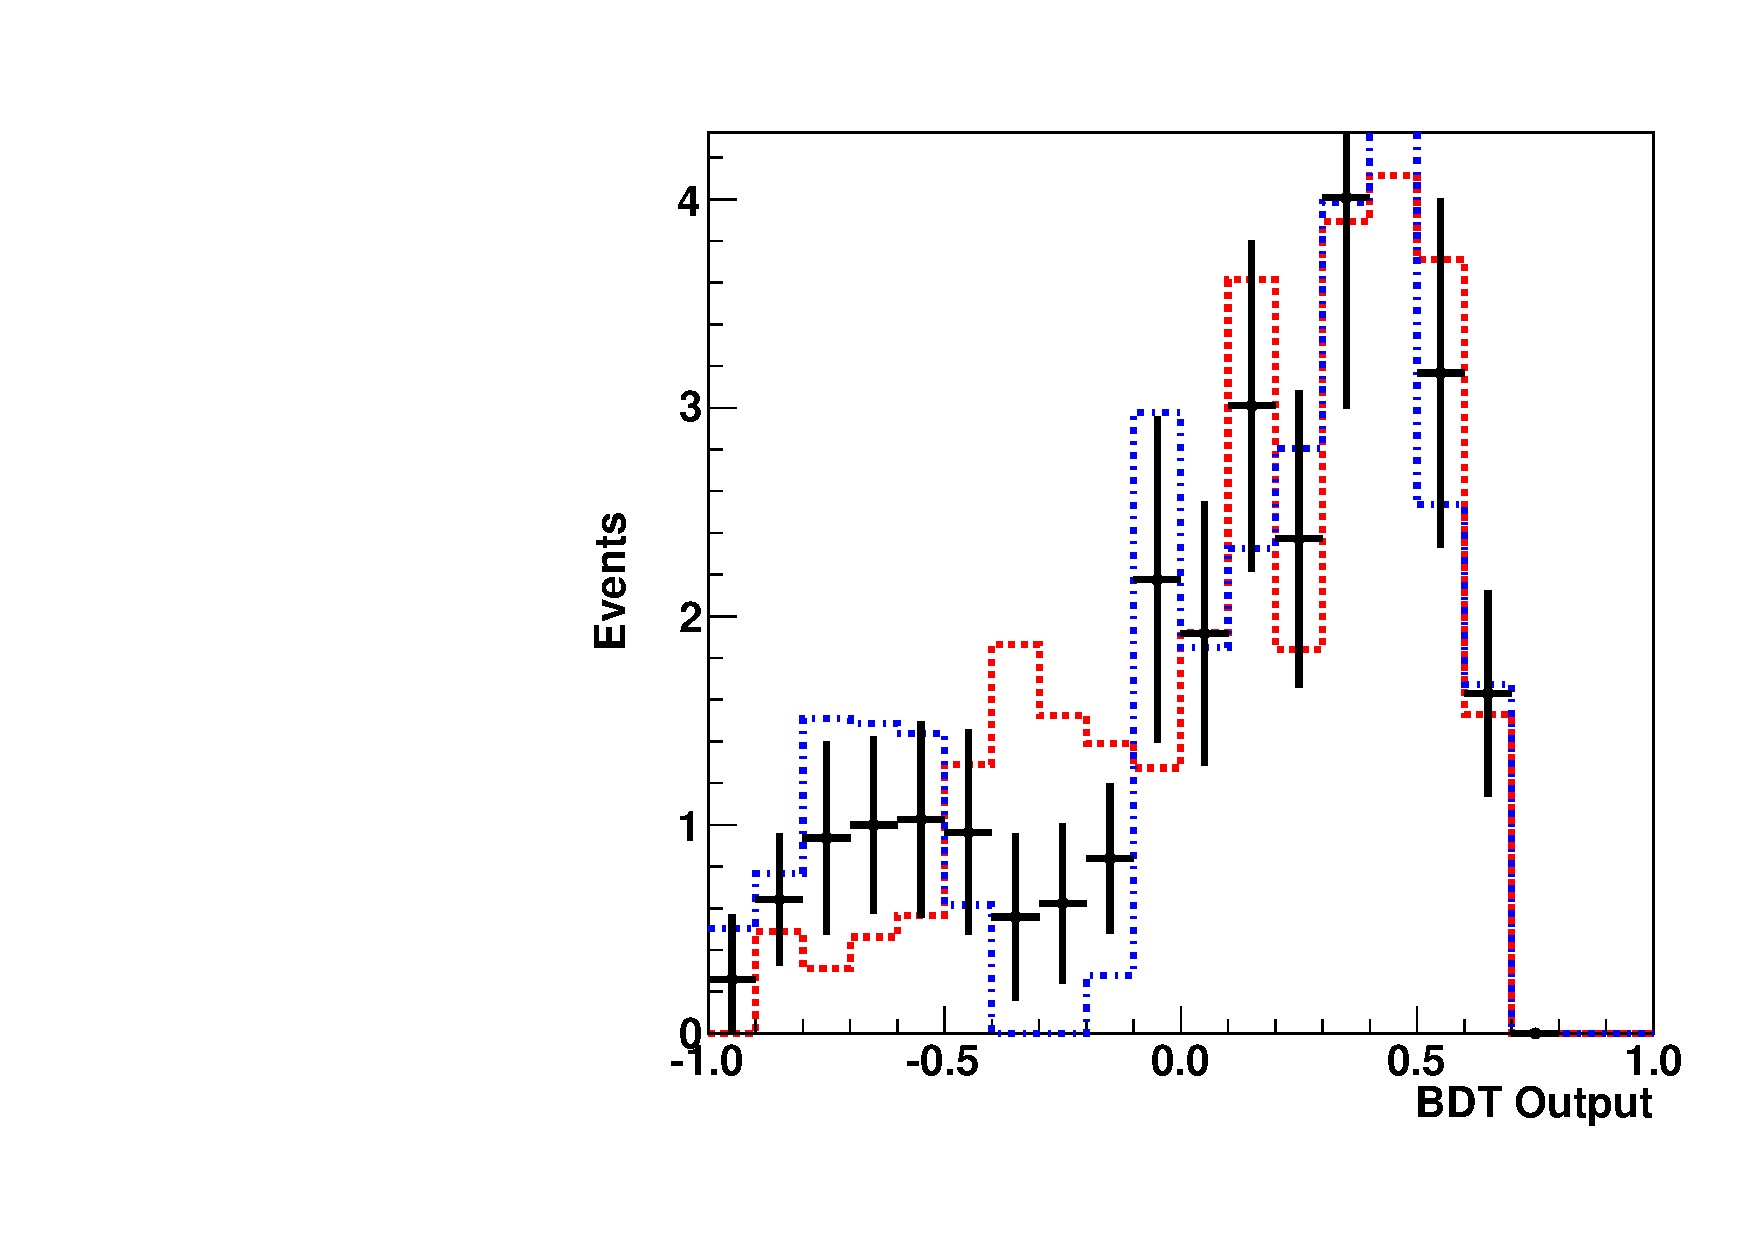
\includegraphics[width=0.49\textwidth]{figures/cvswwof_57.pdf}}
\caption{BDT Output distribution for $H(130) \to \WW$ 0-jet bin analysis opposite-flavor 
final state in $\Wjets$ events for $\mathcal{L}~=~1.55~\pm~0.07~\ifb$. The dots histogram 
is the default shape, while the dashed red histogram is the ``Up" component and the dashed 
blue histograms is the ``Down" component, for the fake rate uncertainty (a) and for the 
Monte Carlo closure test uncertainty (b).}
\label{fig:WJetsNorn}
\end{center}
\end{figure}

\subsubsection{$\dymm$ and $\dyee$ Backgrounds}
The uncertainty on the normalization of this background is rather larger, as
discussed in~\cite{hww_eps}, on the other hand a shape uncertainty could also be
important. Since the number of available simulated events after the final
selection is rather small, the default distribution is taken from events which 
pass all other requirements, but with Min(projected $\met$, projected
track-$\met$) between 20 and 40 $\GeV$, with the normalization obtained from the
signal region evaluation. To have a conservative estimate of the
uncertainty, we take the ``up" variation using the simulated events passing all
requirements, while the mirror of the ratio between the ``up" and default
distributions is the ``down" variation. 

\subsubsection{Top Background}
To account for possible shape uncertainties on the modelling of top simulated
events, we compare different simulated samples with respect to the default ones 
to build the ``up" variation, while the mirror of the ratio between the ``up" 
and default distributions is the ``down" variation. In particular, for $\ttbar$
events we use Madgraph simulated events (Powheg is the default generator), while
for the $\tw$ process we use a sample with different matching procedure.
An example of the effect of this uncertainty is shown in Figure~\ref{fig:topNorm}. 

\begin{figure}[!htbp]
\begin{center}
\subfigure[]{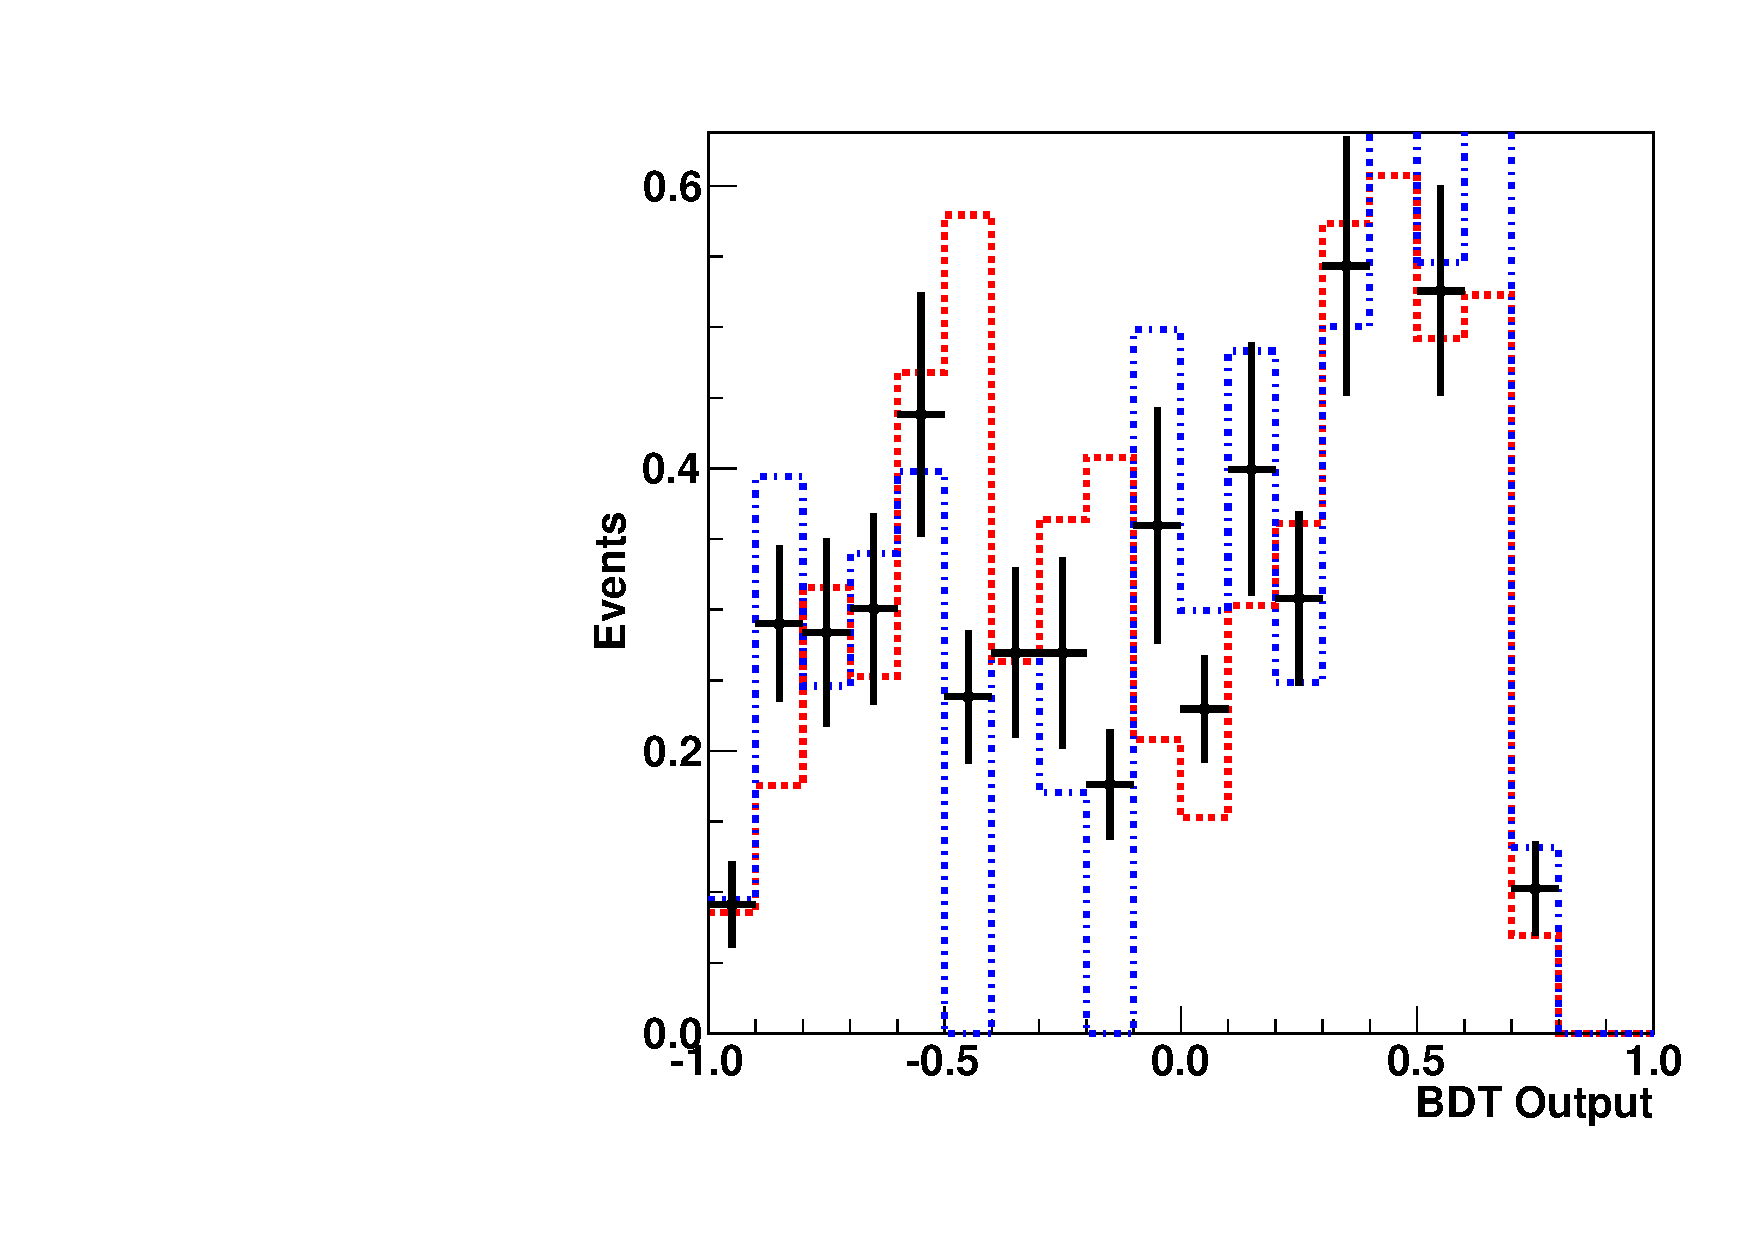
\includegraphics[width=0.49\textwidth]{figures/cvswwof_1.pdf}}
\subfigure[]{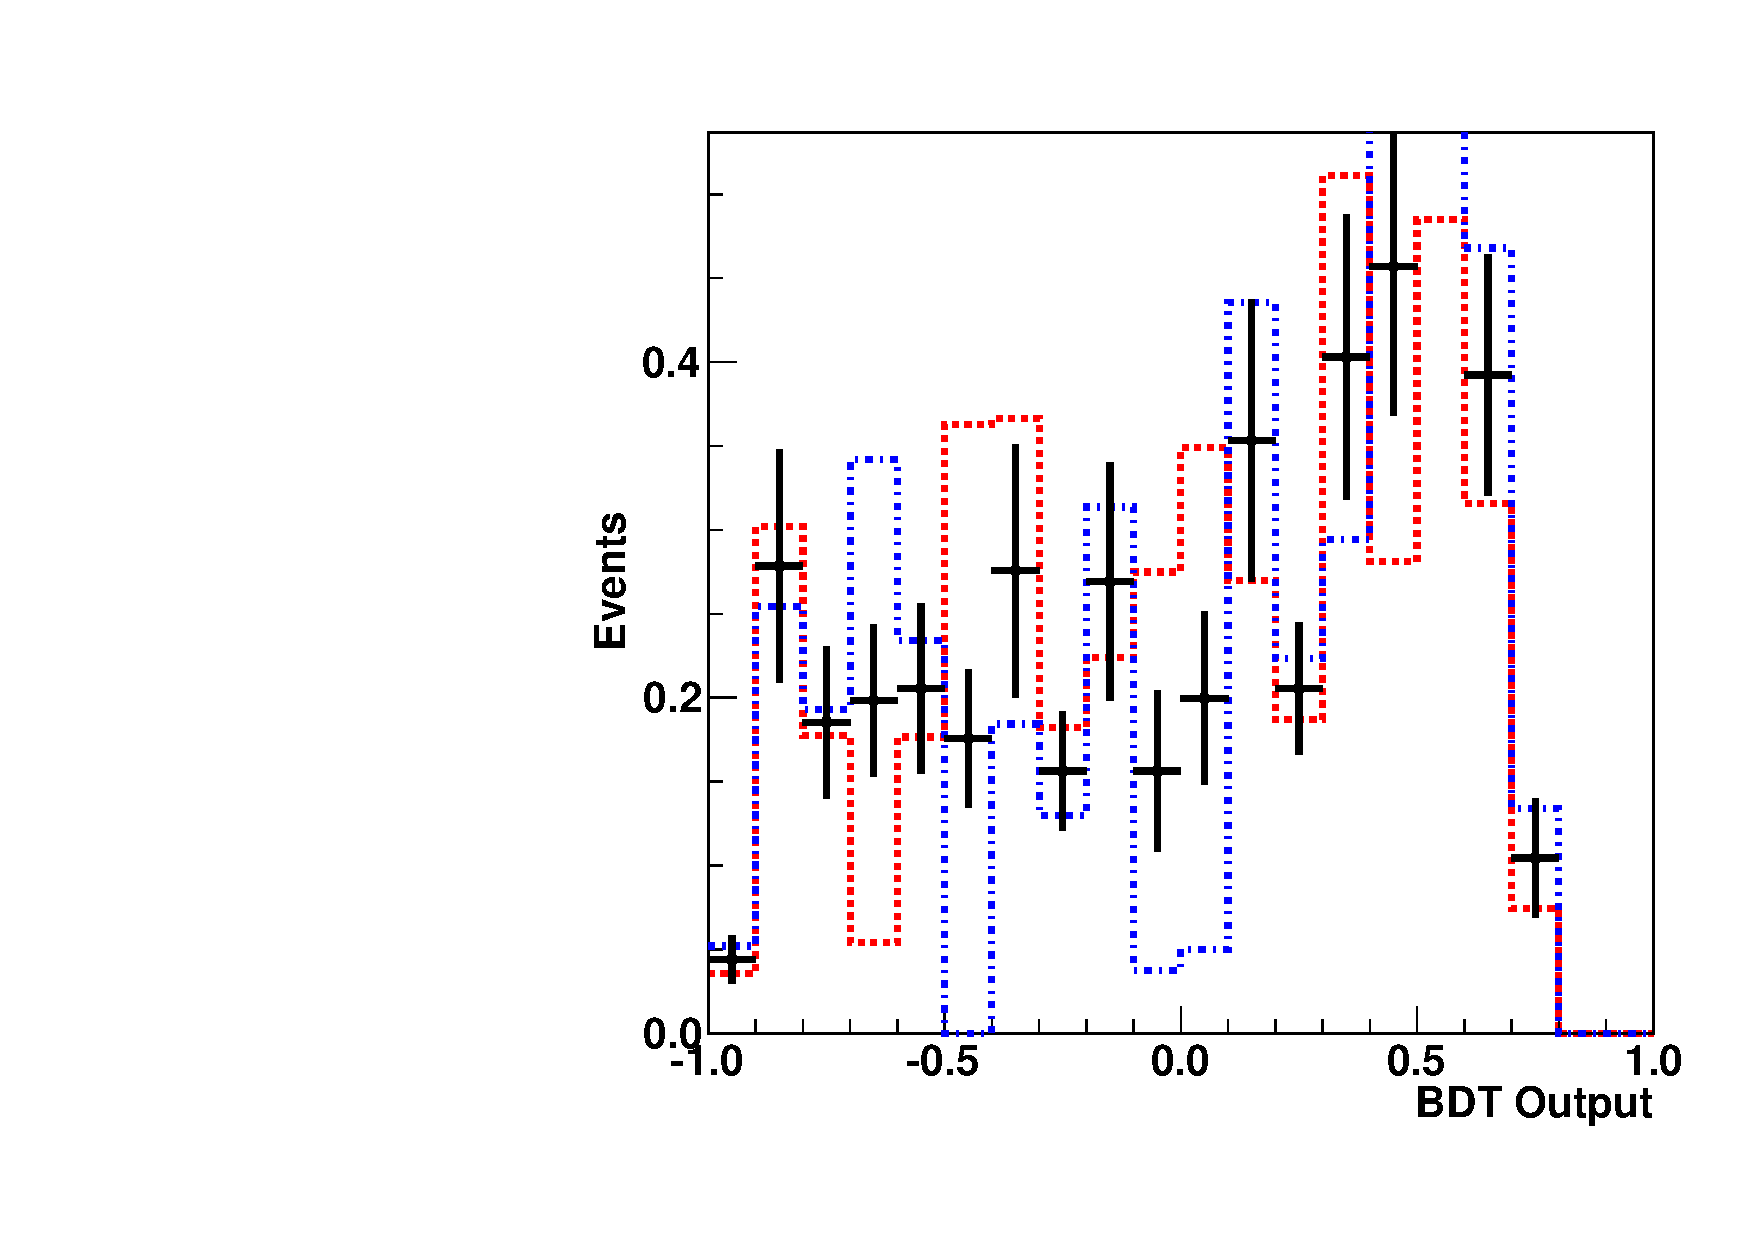
\includegraphics[width=0.49\textwidth]{figures/cvswwsf_1.pdf}}
\caption{BDT Output distribution for $H(130) \to \WW$ 0-jet bin analysis in top events 
for $\mathcal{L}~=~1.55~\pm~0.07~\ifb$. Opposite-flavor (a) and same-flavor (b) final states 
are shown. The dots histogram is the default shape, while the dashed red histogram 
is the ``Up" component and the dashed blue histograms is the ``Down" component, for top 
shape uncertainty.}
\label{fig:topNorm}
\end{center}
\end{figure}

\subsubsection{$\W+\gamma$ Background}
The $\W+\gamma$ background is rather small after our tight preselection
requirements, therefore we do not assign any specific uncertainty due to this
background. The only point to notice is that we take the shape of this process
from a sample of simulated events where the conversion rejection requirements
have been loosened, so that the amount of events used in the final discriminant
variable is larger. We have verified that the shapes do not changed by modifying
those veto requirements within the statistical uncertainties.

\subsubsection{$\dytt$ Background}
The $\dytt$ background is estimated from data using the so-called $\tau$
embedding method. The aim of this method is to create hybrid events with two 
muons (or electrons) coming from a data $\Z$ decay replaced by two 
(simulated) $\tau$ particles. Different techniques for creating such events
exist to replace the muons: either at offline level, at the reconstruction 
level or at the digitazitation level. In addition to the use of data to a very
large extent, this method allows for an increase on the statistical power of the
sample leading to much smaller statistical uncertainties.

\subsubsection{Bin-By-Bin Statistical Uncertainty}
As already stated in Section~\ref{sec:methods}, the current available official 
framework do not support a full proper treatment of the statistical 
uncertainties on each bin independently of the discriminant variable. A way to
account for most of the effect is to build ``up" (``down") variation as the
+1(-1)$\sigma$ statistical uncertainty on every bin. In this way, we properly
consider the uncertainty on every bin, although in a correlated way. 
An example of the effect of this uncertainty is shown in Figure~\ref{fig:qqWWStat}. 

\begin{figure}[!htbp]
\begin{center}
\subfigure[]{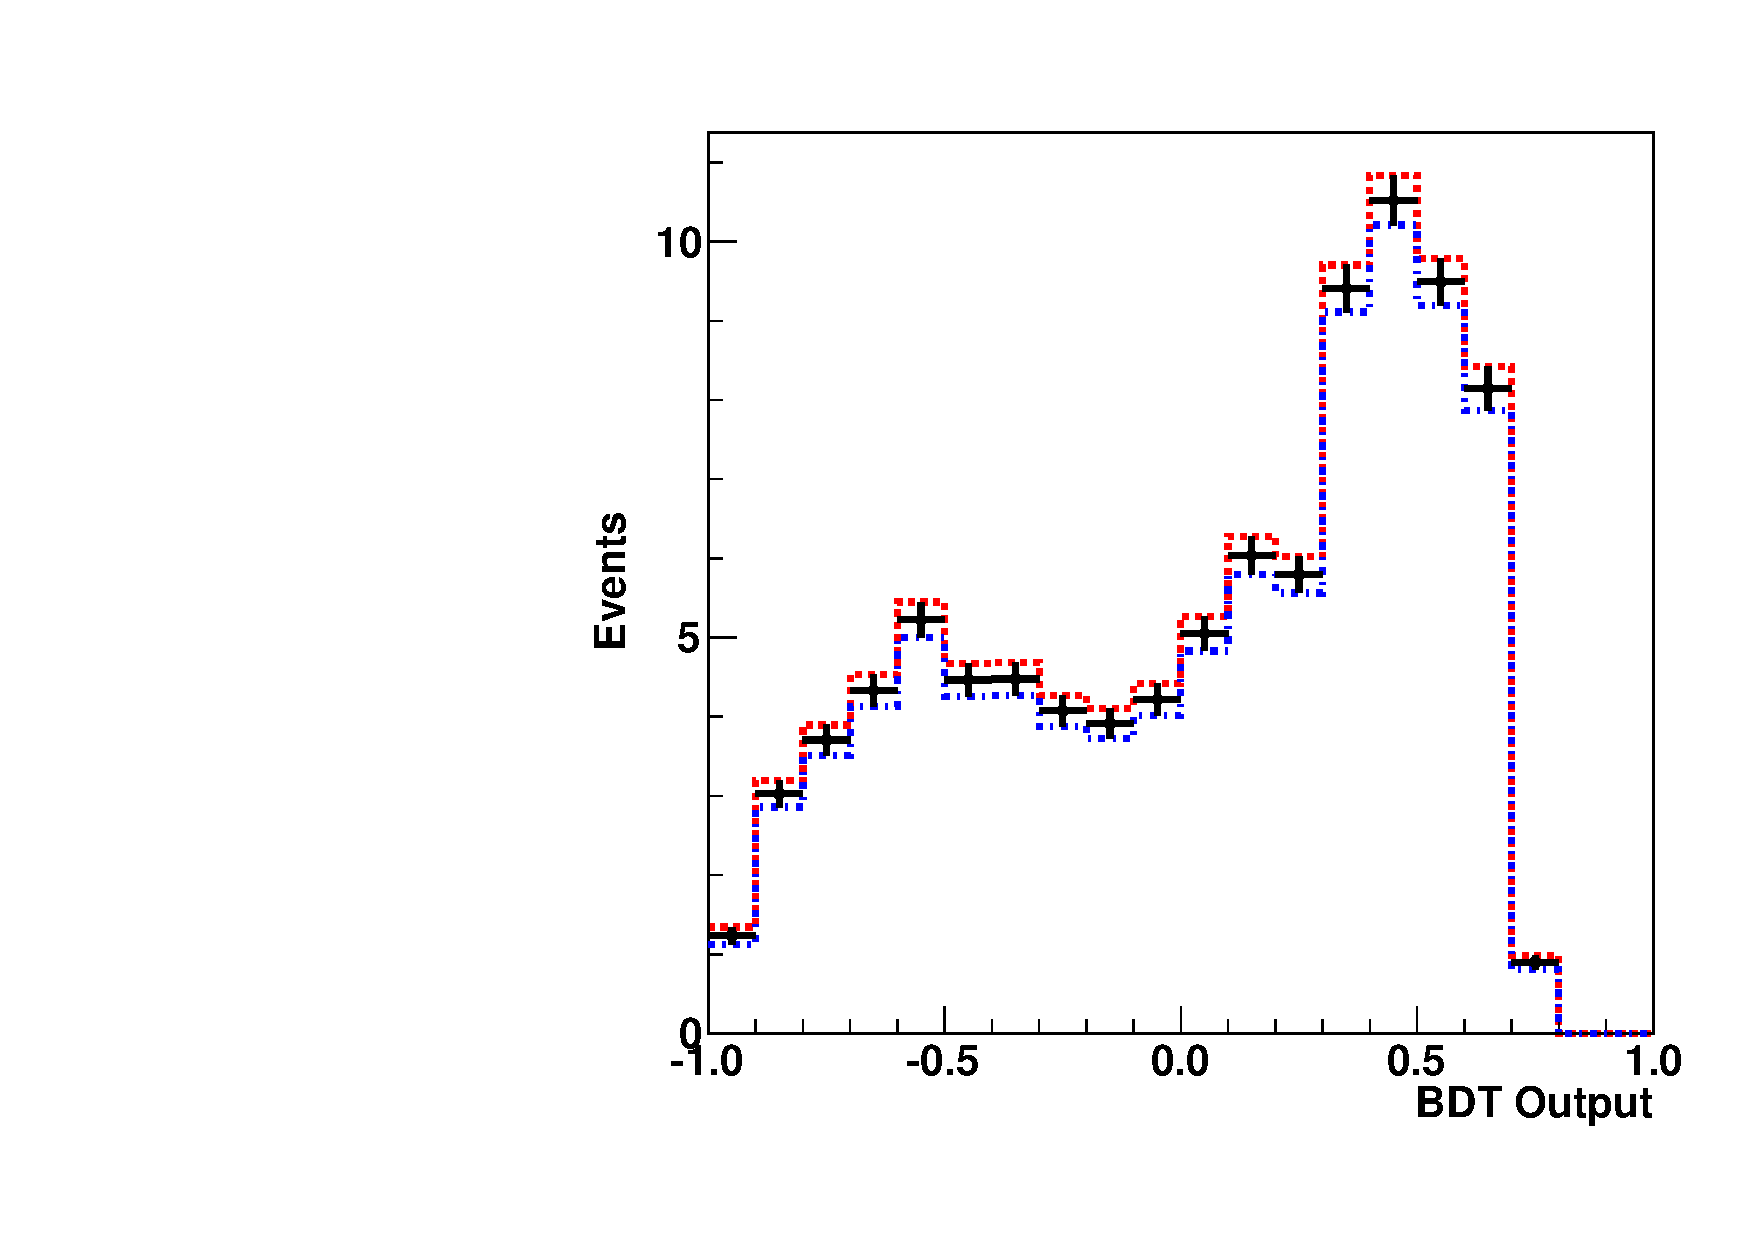
\includegraphics[width=0.49\textwidth]{figures/cvswwof_7.pdf}}
\subfigure[]{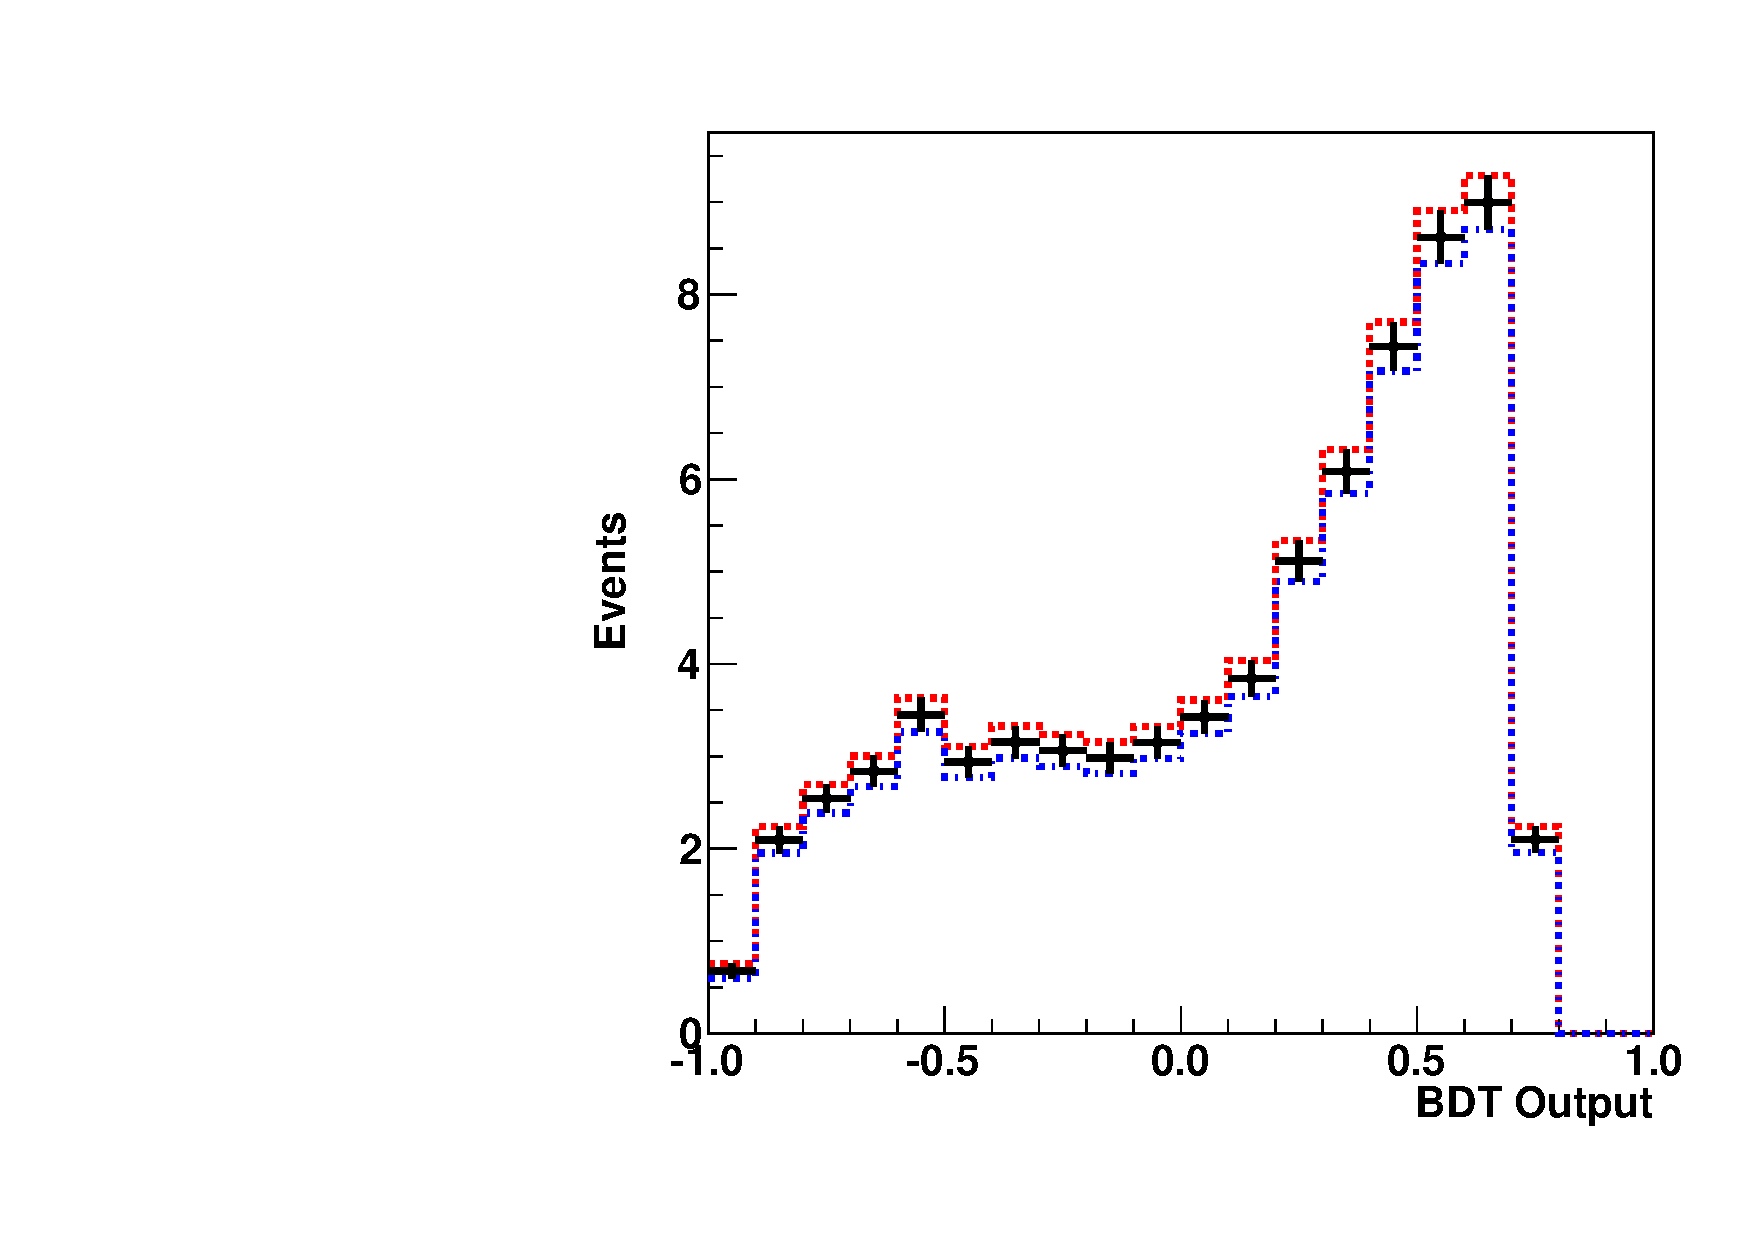
\includegraphics[width=0.49\textwidth]{figures/cvswwsf_7.pdf}}
\caption{BDT Output distribution for $H(130) \to \WW$ 0-jet bin analysis in $qq \to \WW$ events 
for $\mathcal{L}~=~1.55~\pm~0.07~\ifb$. Opposite-flavor (a) and same-flavor (b) final states 
are shown. The dots histogram is the default shape, while the dashed red histogram 
is the ``Up" component and the dashed blue histograms is the ``Down" component, for statistical 
shape uncertainty.}
\label{fig:qqWWStat}
\end{center}
\end{figure}

As a cross-check, we perform the following: (a) we divide the discriminant
variable into 3 regions (low, medium, and high values), (b) for the ``up" 
variation we move all low points up by one $\sigma$ and all high points down 
by one $\sigma$, (c) for the "down" variation we do the opposite. With this
procedure we create an artificial shape variation due to the statistical
uncertainties. It is a conservative approach, but it gives an idea of the size of
the effect. 
An example of the effect of this uncertainty is shown in Figure~\ref{fig:qqWWStatAlt}. 

\begin{figure}[!htbp]
\begin{center}
\subfigure[]{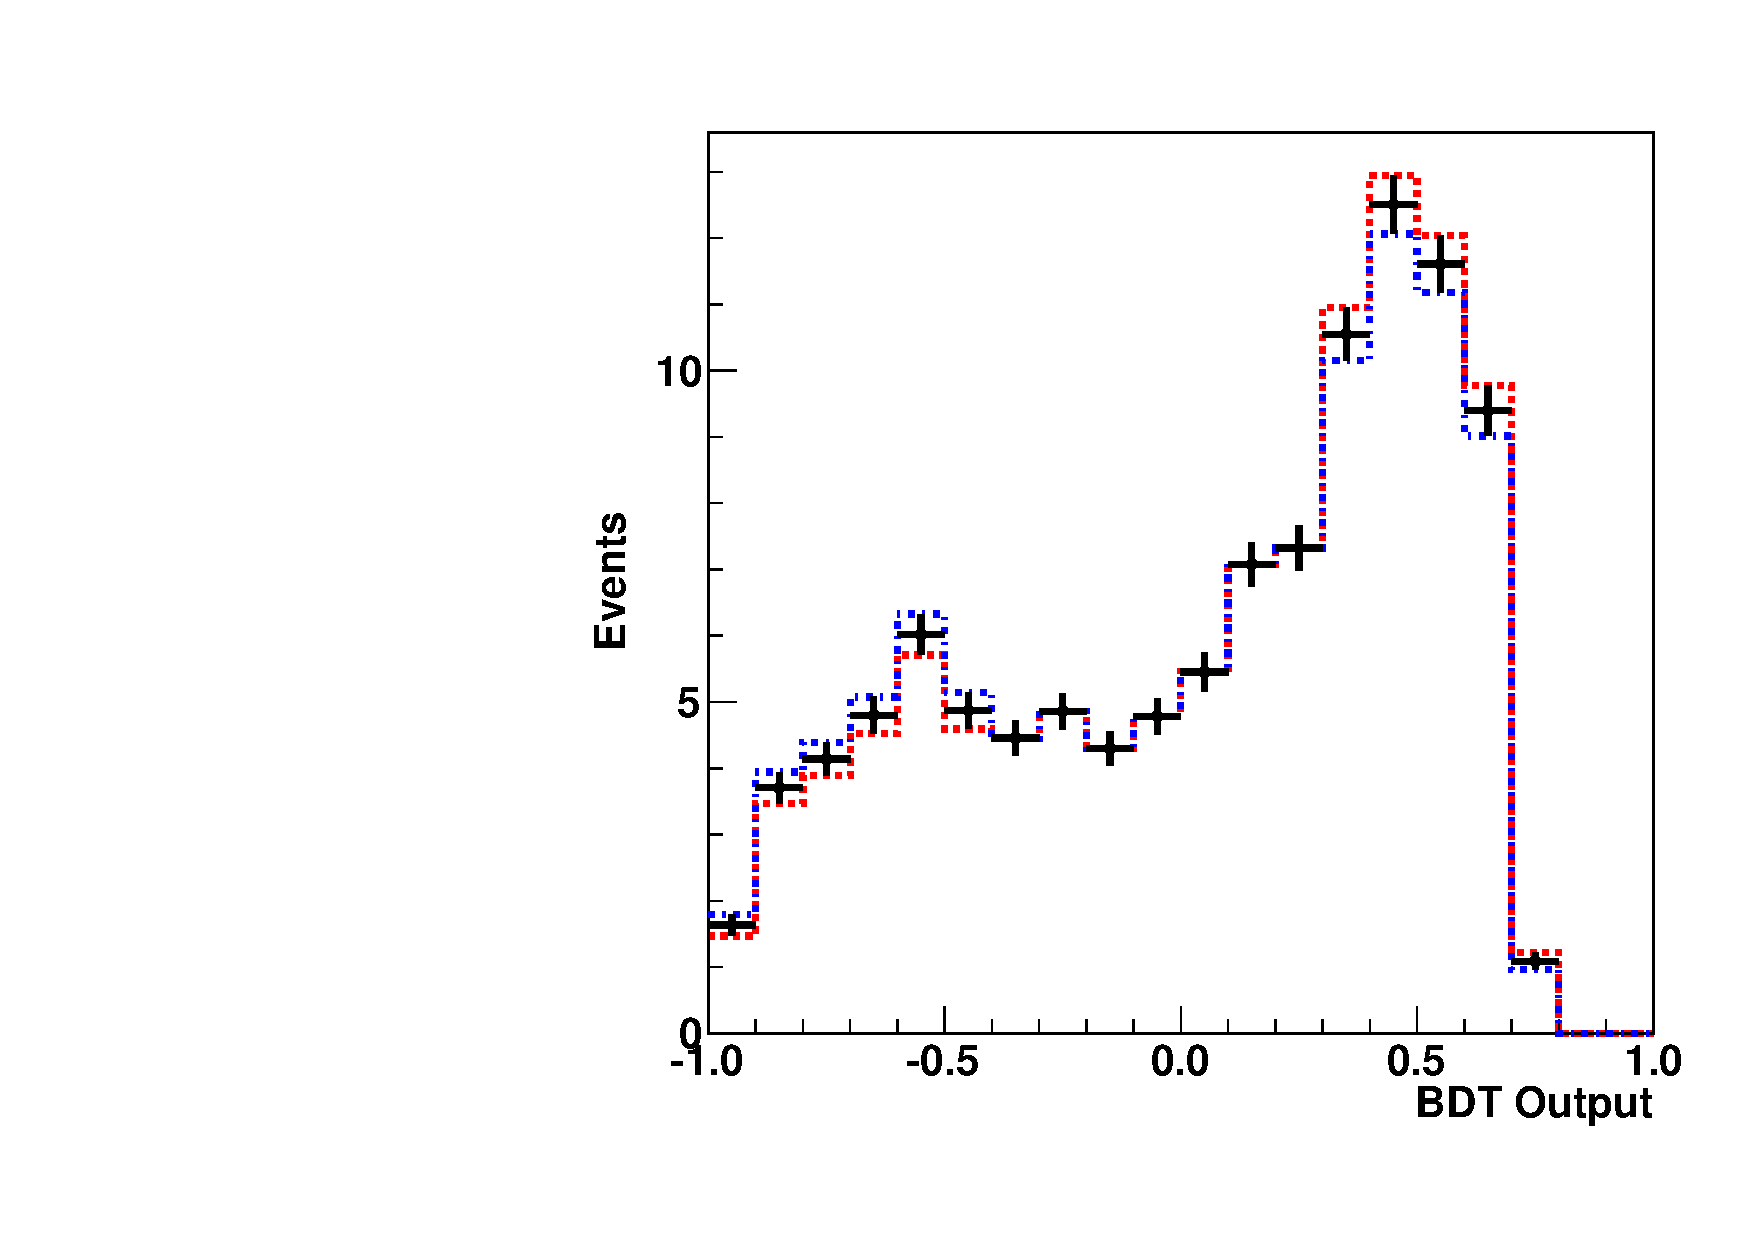
\includegraphics[width=0.49\textwidth]{figures/cvswwof_7_alt.pdf}}
\subfigure[]{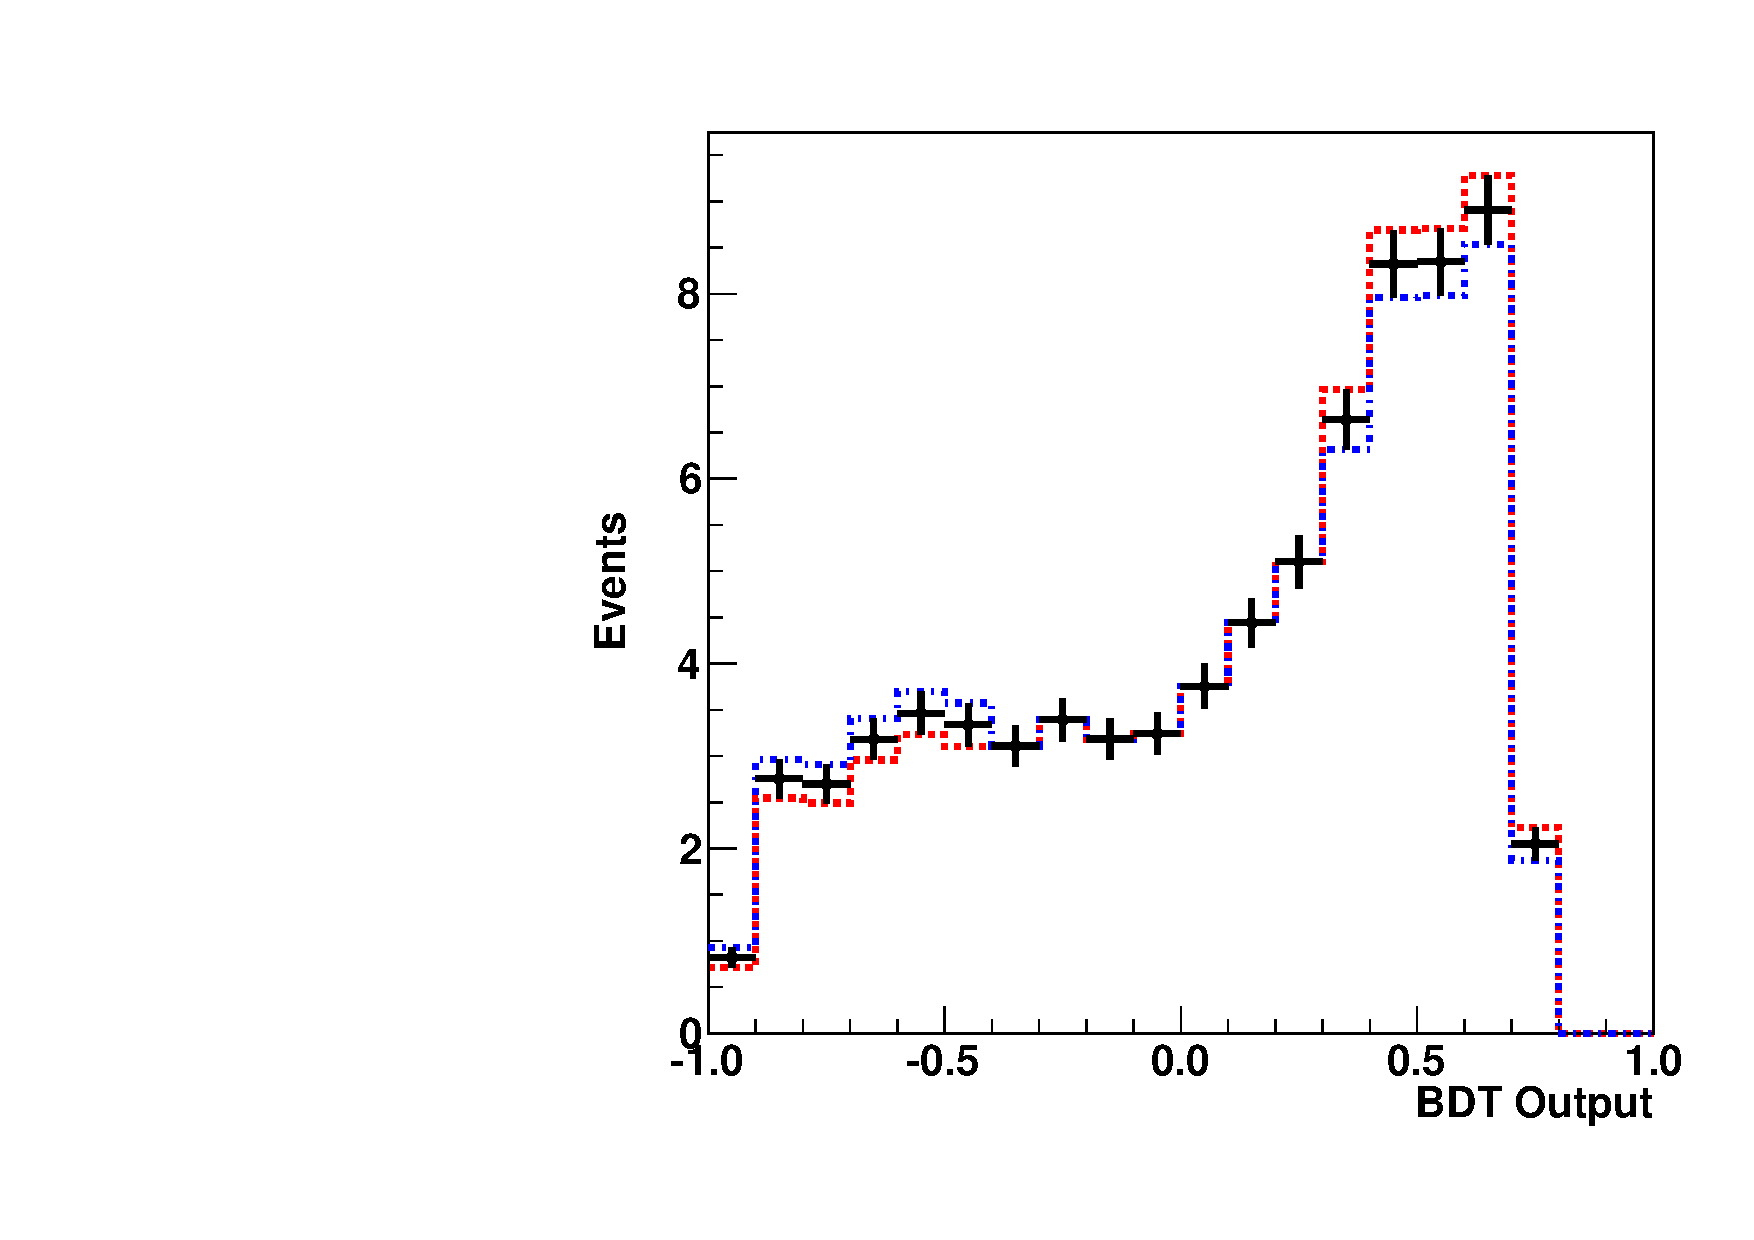
\includegraphics[width=0.49\textwidth]{figures/cvswwsf_7_alt.pdf}}
\caption{BDT Output distribution for $H(130) \to \WW$ 0-jet bin analysis in $qq \to \WW$ events 
for $\mathcal{L}~=~1.55~\pm~0.07~\ifb$. Opposite-flavor (a) and same-flavor (b) final states 
are shown. The dots histogram is the default shape, while the dashed red histogram 
is the ``Up" component and the dashed blue histograms is the ``Down" component, for statistical 
shape uncertainty using an alternative approach.}
\label{fig:qqWWStatAlt}
\end{center}
\end{figure}


\subsection{Validation tests}
  \label{sec:validation_ww}
  To validate the procedures discussed in the previous section, detailed studies 
have been carried out using a data sample of $\mathcal{L}~=~1.55~\pm~0.07~\ifb$,
corresponding to the available dataset for the Lepton-Photon 2011 conference. We
use simulated events from the newer Summer11 CMSSW\_4\_2\_X production, and
therefore the whole analysis chain was re-evaluated. Nevertheless, small changes
were observed with respect to the results obtained earlier.

\subsubsection{Shape vs. Counting Analyses}
A first interesting study is to compare the improvement in the performance by
using the shape of a discriminant variable with respect to a simple
cut-and-count analysis. There is no single very powerful distribution, like
$m_{\gamma\gamma}$ for the $\Hi \to \gamma\gamma$ case, in this dilepton
final state. Nevertheless, we want to show that the major gain is coming from the
use of the shape of a discriminant variable, and not just by the use of the
correlations among different variables in a multivariate classifier, e.g. Boost
Decision Tree (BDT).

Table~\ref{tab:mvaseveral} shows the median expected cross section ratio 
limits for several approaches as a function of the Higgs mass. First, we see
that the BDT shape analysis is always about 30-40\% better than the simple
cut-based approach~\footnote{The systematic uncertainties related to the
shape variation of the multivariate classifier are not considered here, the full
comparision will be shown in the following section.}. 
Second, we see that a multivariate likelihood approach, 
where the correlations among the different variables are not used, gives a
degradation in the performance of about 10\% only with respect to the BDT
approach. Finally, we see that the use of single discriminant variables, like 
either $\mll$ or $\delphill$, gives a performance comparable to the likelihood
approach, and always better than the cut-based analysis. Therefore, the 
main improvement comes from the use of the shape of a discriminant variable, 
not by the correlations among the variables of the multivariate BDT approach.

\begin{table}[!ht]
  \begin{center}
 {\small
  \begin{tabular} {|c|c|c|c|c|c|c|c|c|}
  \hline
mass       & BDT  & likelihood  & cut-based &  \multicolumn{5}{c|}{single variable} \\
$[\GeVcc]$ &      &             &           &  $\mll$  & $m_{T}$  & $\delphill$  & $\pt^{\ell\ell}$  & $\pt^{leading}$ \\
  \hline
115 & 3.30 & 3.70 & 4.74 & 3.69 &  5.97 & 4.92 &  6.27 & 6.41 \\
120 & 2.03 & 2.27 & 2.82 & 2.21 &  3.42 & 2.95 &  3.57 & 3.65 \\
130 & 0.97 & 1.11 & 1.30 & 1.06 &  1.61 & 1.35 &  1.69 & 1.63 \\
140 & 0.62 & 0.70 & 0.78 & 0.69 &  0.99 & 0.83 &  1.04 & 0.98 \\
150 & 0.40 & 0.45 & 0.53 & 0.50 &  0.64 & 0.57 &  0.69 & 0.64 \\
160 & 0.22 & 0.26 & 0.30 & 0.35 &  0.42 & 0.37 &  0.44 & 0.42 \\
170 & 0.25 & 0.28 & 0.32 & 0.41 &  0.40 & 0.40 &  0.41 & 0.46 \\
180 & 0.39 & 0.44 & 0.50 & 0.63 &  0.52 & 0.60 &  0.55 & 0.63 \\
190 & 0.59 & 0.68 & 0.72 & 0.98 &  0.77 & 0.94 &  0.80 & 0.91 \\
200 & 0.80 & 0.90 & 0.97 & 1.29 &  1.00 & 1.30 &  1.02 & 1.13 \\
250 & 1.34 & 1.45 & 1.87 & 1.71 &  1.99 & 2.25 &  2.05 & 1.66 \\
300 & 1.51 & 1.60 & 2.19 & 1.84 &  2.64 & 2.21 &  2.77 & 1.77 \\
350 & 1.40 & 1.47 & 2.09 & 1.75 &  2.63 & 1.94 &  2.84 & 1.60 \\
400 & 1.52 & 1.65 & 2.29 & 1.93 &  2.98 & 2.12 &  3.29 & 1.72 \\
450 & 2.14 & 2.30 & 3.01 & 2.71 &  3.93 & 3.01 &  4.52 & 2.35 \\
500 & 3.15 & 3.43 & 4.44 & 4.00 &  5.54 & 4.52 &  6.27 & 3.46 \\
550 & 4.53 & 4.96 & 6.15 & 5.54 &  7.85 & 6.44 &  9.04 & 4.72 \\
600 & 6.60 & 7.14 & 9.07 & 8.03 & 10.96 & 9.51 & 12.76 & 6.82 \\
  \hline
  \end{tabular}
  \caption{Median expected cross section ratio limits for several 
  approaches as a function of the Higgs mass.}
  \label{tab:mvaseveral}
  }
  \end{center}
\end{table}

\subsubsection{Inclusion of Shape Uncertainties}
The median expected cross section ratio limits as a function 
of the Higgs mass, together with the 1/2-$\sigma$ uncertainty bands, for the 
Lepton-Photon 2011 dataset, after the inclusion of all the shape uncertainties 
are summarized in this section. Table~\ref{tab:mva_shapewithwithout} shows the effect 
on the results by including such uncertainties, while Table~\ref{tab:mva_shapevscuts} 
compares them with the cut-based approach. In summary, we see that the median expected 
limit is barely unaffected by the inclusion of these shape uncertainties, while 
the uncertainty bands get wider by $\sim$10-15\%. Therefore, the $\sim$30\% 
increase in the performance with respect to the cut-based analysis remains after the 
inclusion of such effects.

In order to study the effect of some uncertainties, we exclude some of them and 
recompute the limits. Tables~\ref{tab:mva_shapewithwithoutww},
~\ref{tab:mva_shapewithwithoutstat} and~\ref{tab:mva_shapewithwithoutlepjes} compare 
the default analysis with the one excluding the $\WW$ shape uncertainties, the statistical 
uncertainties and the lepton and jet energy shape uncertainties, respectively. All 
of them show a sizable, but not dominant, effect. Therefore we should consider them all. 
Finally, we compare in Table~\ref{tab:mva_shapealtstat} the default analysis with 
the one using an alternative approach for the evaluation of the statistical uncertainty, as 
described in Section~\ref{sec:systematic_ww}. No large degradation on the expected limits 
is seen.

\begin{table}[!ht]
\begin{center}
{\normalsize
\begin{tabular}{|l|c|c|c|c|c|c|}
\hline
      &  \multicolumn{3}{c|}{without shape uncertainties} &\multicolumn{3}{c|}{with shape uncertainties} \\
\hline
Mass  &  Median      &     68\% C.L. band &  95\% C.L. band &  Median	   &	 68\% C.L. band &  95\% C.L. band\\
      &  Expected    &                    &                 &  Expected    &			&		 \\
\hline
115 &  3.3 & [2.3, 4.8] & [1.7, 6.8]  &  3.3 & [2.1, 5.1] & [1.5, 7.6] \\
120 &  2.0 & [1.4, 3.0] & [1.0, 4.1]  &  2.0 & [1.3, 3.1] & [0.9, 4.5] \\
130 &  0.9 & [0.7, 1.4] & [0.5, 1.9]  &  0.9 & [0.6, 1.5] & [0.4, 2.2] \\
140 &  0.6 & [0.4, 0.9] & [0.3, 1.2]  &  0.6 & [0.4, 0.9] & [0.2, 1.3] \\
150 &  0.4 & [0.3, 0.6] & [0.2, 0.8]  &  0.4 & [0.2, 0.6] & [0.2, 0.8] \\
160 &  0.3 & [0.2, 0.3] & [0.1, 0.5]  &  0.2 & [0.1, 0.3] & [0.1, 0.5] \\
170 &  0.3 & [0.2, 0.4] & [0.1, 0.5]  &  0.2 & [0.1, 0.4] & [0.1, 0.6] \\
180 &  0.4 & [0.3, 0.6] & [0.2, 0.8]  &  0.4 & [0.2, 0.6] & [0.1, 0.9] \\
190 &  0.6 & [0.4, 0.9] & [0.3, 1.2]  &  0.5 & [0.3, 0.9] & [0.2, 1.3] \\
200 &  0.8 & [0.5, 1.2] & [0.4, 1.7]  &  0.7 & [0.4, 1.2] & [0.3, 1.9] \\
250 &  1.3 & [0.9, 2.0] & [0.7, 2.8]  &  1.4 & [0.9, 2.2] & [0.6, 3.2] \\
300 &  1.5 & [1.1, 2.2] & [0.8, 3.1]  &  1.5 & [1.0, 2.3] & [0.7, 3.5] \\
350 &  1.4 & [1.0, 2.0] & [0.7, 2.8]  &  1.4 & [0.9, 2.2] & [0.6, 3.1] \\
400 &  1.5 & [1.1, 2.1] & [0.8, 2.9]  &  1.5 & [1.0, 2.3] & [0.7, 3.3] \\
450 &  2.1 & [1.4, 3.0] & [1.1, 4.2]  &  2.0 & [1.4, 3.1] & [1.0, 4.5] \\
500 &  3.0 & [2.1, 4.2] & [1.6, 5.9]  &  3.0 & [2.0, 4.5] & [1.4, 6.5] \\
550 &  4.1 & [2.9, 5.9] & [2.2, 8.3]  &  4.1 & [2.8, 6.2] & [2.0, 8.9] \\
600 &  5.6 & [4.0, 8.0] & [3.0, 11.1] &  5.6 & [3.9, 8.4] & [2.8, 12.2]\\
\hline
\end{tabular}
}
\caption{Comparison of the median expected cross section ratio limits as a function 
of the Higgs mass, together with the 1/2-$\sigma$ uncertainty bands, without and with the 
shape uncertainties considered.}
\label{tab:mva_shapewithwithout}
\end{center}
\end{table}

\begin{table}[!ht]
\begin{center}
{\normalsize
\begin{tabular}{|l|c|c|c|c|c|c|}
\hline
      &  \multicolumn{3}{c|}{cut-based analysis} &\multicolumn{3}{c|}{BDT shape analysis} \\
\hline
Mass  &  Median      &     68\% C.L. band &  95\% C.L. band &  Median	   &	 68\% C.L. band &  95\% C.L. band\\
      &  Expected    &                    &                 &  Expected    &			&		 \\
\hline
115 &  4.7 & [3.0, 7.3] & [1.8, 11.0] &  3.3 & [2.1, 5.1] & [1.5, 7.6] \\
120 &  2.8 & [1.8, 4.3] & [1.1, 6.3]  &  2.0 & [1.3, 3.1] & [0.9, 4.5] \\
130 &  1.3 & [0.9, 1.9] & [0.6, 2.8]  &  0.9 & [0.6, 1.5] & [0.4, 2.2] \\
140 &  0.8 & [0.5, 1.2] & [0.4, 1.6]  &  0.6 & [0.4, 0.9] & [0.2, 1.3] \\
150 &  0.5 & [0.4, 0.8] & [0.2, 1.1]  &  0.4 & [0.2, 0.6] & [0.2, 0.8] \\
160 &  0.3 & [0.2, 0.4] & [0.1, 0.7]  &  0.2 & [0.1, 0.3] & [0.1, 0.5] \\
170 &  0.3 & [0.2, 0.5] & [0.2, 0.7]  &  0.2 & [0.1, 0.4] & [0.1, 0.6] \\
180 &  0.5 & [0.3, 0.8] & [0.2, 1.1]  &  0.4 & [0.2, 0.6] & [0.1, 0.9] \\
190 &  0.7 & [0.5, 1.1] & [0.4, 1.5]  &  0.5 & [0.3, 0.9] & [0.2, 1.3] \\
200 &  1.0 & [0.7, 1.4] & [0.5, 2.0]  &  0.7 & [0.4, 1.2] & [0.3, 1.9] \\
250 &  1.9 & [1.3, 2.7] & [0.9, 3.8]  &  1.4 & [0.9, 2.2] & [0.6, 3.2] \\
300 &  2.2 & [1.5, 3.1] & [1.1, 4.4]  &  1.5 & [1.0, 2.3] & [0.7, 3.5] \\
350 &  2.1 & [1.4, 3.0] & [1.0, 4.2]  &  1.4 & [0.9, 2.2] & [0.6, 3.1] \\
400 &  2.3 & [1.6, 3.3] & [1.1, 4.6]  &  1.5 & [1.0, 2.3] & [0.7, 3.3] \\
450 &  2.9 & [2.0, 4.1] & [1.5, 6.0]  &  2.0 & [1.4, 3.1] & [1.0, 4.5] \\
500 &  4.1 & [2.9, 6.0] & [2.1, 8.4]  &  3.0 & [2.0, 4.5] & [1.4, 6.5] \\
550 &  5.5 & [3.9, 8.0] & [2.8, 11.3] &  4.1 & [2.8, 6.2] & [2.0, 8.9] \\
600 &  7.6 & [5.4, 11.1]& [4.0, 15.5] &  5.6 & [3.9, 8.4] & [2.8, 12.2]\\
\hline
\end{tabular}
}
\caption{Comparison of the median expected cross section ratio limits as a function 
of the Higgs mass, together with the 1/2-$\sigma$ uncertainty bands, for the cut-based analysis 
and the full BDT shape analysis.}
\label{tab:mva_shapevscuts}
\end{center}
\end{table}

\begin{table}[!ht]
\begin{center}
{\normalsize
\begin{tabular}{|l|c|c|c|c|c|c|}
\hline
      &  \multicolumn{3}{c|}{without $\WW$ shape uncertainties} &\multicolumn{3}{c|}{BDT shape analysis} \\
\hline
Mass  &  Median      &     68\% C.L. band &  95\% C.L. band &  Median	   &	 68\% C.L. band &  95\% C.L. band\\
      &  Expected    &                    &                 &  Expected    &			&		 \\
\hline
115 &  3.3 & [2.2, 5.1] & [1.5, 7.5]  &  3.3 & [2.1, 5.1] & [1.5, 7.6] \\
120 &  2.1 & [1.4, 3.1] & [0.9, 4.5]  &  2.0 & [1.3, 3.1] & [0.9, 4.5] \\
130 &  1.0 & [0.6, 1.4] & [0.4, 2.1]  &  0.9 & [0.6, 1.5] & [0.4, 2.2] \\
140 &  0.6 & [0.4, 0.9] & [0.3, 1.3]  &  0.6 & [0.4, 0.9] & [0.2, 1.3] \\
150 &  0.4 & [0.2, 0.6] & [0.2, 0.8]  &  0.4 & [0.2, 0.6] & [0.2, 0.8] \\
160 &  0.2 & [0.1, 0.3] & [0.1, 0.5]  &  0.2 & [0.1, 0.3] & [0.1, 0.5] \\
170 &  0.2 & [0.1, 0.4] & [0.1, 0.6]  &  0.2 & [0.1, 0.4] & [0.1, 0.6] \\
180 &  0.4 & [0.2, 0.6] & [0.1, 0.8]  &  0.4 & [0.2, 0.6] & [0.1, 0.9] \\
190 &  0.5 & [0.3, 0.9] & [0.2, 1.3]  &  0.5 & [0.3, 0.9] & [0.2, 1.3] \\
200 &  0.7 & [0.4, 1.2] & [0.3, 1.8]  &  0.7 & [0.4, 1.2] & [0.3, 1.9] \\
250 &  1.3 & [0.9, 2.0] & [0.6, 2.9]  &  1.4 & [0.9, 2.2] & [0.6, 3.2] \\
300 &  1.5 & [1.0, 2.3] & [0.7, 3.3]  &  1.5 & [1.0, 2.3] & [0.7, 3.5] \\
350 &  1.4 & [0.9, 2.1] & [0.6, 3.1]  &  1.4 & [0.9, 2.2] & [0.6, 3.1] \\
400 &  1.5 & [1.0, 2.3] & [0.7, 3.2]  &  1.5 & [1.0, 2.3] & [0.7, 3.3] \\
450 &  2.1 & [1.4, 3.1] & [1.0, 4.5]  &  2.0 & [1.4, 3.1] & [1.0, 4.5] \\
500 &  3.0 & [2.1, 4.5] & [1.5, 6.4]  &  3.0 & [2.0, 4.5] & [1.4, 6.5] \\
550 &  4.2 & [2.9, 6.1] & [2.1, 8.6]  &  4.1 & [2.8, 6.2] & [2.0, 8.9] \\
600 &  5.7 & [3.9, 8.3] & [2.8, 12.0] &  5.6 & [3.9, 8.4] & [2.8, 12.2]\\
\hline
\end{tabular}
}
\caption{Comparison of the median expected cross section ratio limits as a function 
of the Higgs mass, together with the 1/2-$\sigma$ uncertainty bands, without and with the 
$\WW$ shape uncertainties considered.}
\label{tab:mva_shapewithwithoutww}
\end{center}
\end{table}

\begin{table}[!ht]
\begin{center}
{\normalsize
\begin{tabular}{|l|c|c|c|c|c|c|}
\hline
      &  \multicolumn{3}{c|}{without statistical uncertainties} &\multicolumn{3}{c|}{BDT shape analysis} \\
\hline
Mass  &  Median      &     68\% C.L. band &  95\% C.L. band &  Median	   &	 68\% C.L. band &  95\% C.L. band\\
      &  Expected    &                    &                 &  Expected    &			&		 \\
\hline
115 &  3.3 & [2.2, 4.9] & [1.5, 7.1]  &  3.3 & [2.1, 5.1] & [1.5, 7.6] \\
120 &  2.0 & [1.3, 3.0] & [0.9, 4.4]  &  2.0 & [1.3, 3.1] & [0.9, 4.5] \\
130 &  0.9 & [0.6, 1.4] & [0.4, 2.1]  &  0.9 & [0.6, 1.5] & [0.4, 2.2] \\
140 &  0.6 & [0.4, 0.9] & [0.3, 1.3]  &  0.6 & [0.4, 0.9] & [0.2, 1.3] \\
150 &  0.4 & [0.2, 0.6] & [0.2, 0.8]  &  0.4 & [0.2, 0.6] & [0.2, 0.8] \\
160 &  0.2 & [0.1, 0.3] & [0.1, 0.5]  &  0.2 & [0.1, 0.3] & [0.1, 0.5] \\
170 &  0.2 & [0.1, 0.4] & [0.1, 0.5]  &  0.2 & [0.1, 0.4] & [0.1, 0.6] \\
180 &  0.4 & [0.2, 0.6] & [0.1, 0.9]  &  0.4 & [0.2, 0.6] & [0.1, 0.9] \\
190 &  0.5 & [0.3, 0.9] & [0.2, 1.4]  &  0.5 & [0.3, 0.9] & [0.2, 1.3] \\
200 &  0.7 & [0.4, 1.2] & [0.2, 1.9]  &  0.7 & [0.4, 1.2] & [0.3, 1.9] \\
250 &  1.4 & [0.9, 2.2] & [0.6, 3.3]  &  1.4 & [0.9, 2.2] & [0.6, 3.2] \\
300 &  1.5 & [1.0, 2.3] & [0.7, 3.4]  &  1.5 & [1.0, 2.3] & [0.7, 3.5] \\
350 &  1.4 & [0.9, 2.1] & [0.6, 3.0]  &  1.4 & [0.9, 2.2] & [0.6, 3.1] \\
400 &  1.5 & [1.0, 2.3] & [0.7, 3.3]  &  1.5 & [1.0, 2.3] & [0.7, 3.3] \\
450 &  2.1 & [1.4, 3.1] & [1.0, 4.5]  &  2.0 & [1.4, 3.1] & [1.0, 4.5] \\
500 &  3.0 & [2.0, 4.5] & [1.4, 6.5]  &  3.0 & [2.0, 4.5] & [1.4, 6.5] \\
550 &  4.1 & [2.8, 6.1] & [2.0, 8.8]  &  4.1 & [2.8, 6.2] & [2.0, 8.9] \\
600 &  5.6 & [3.8, 8.2] & [2.7, 11.8] &  5.6 & [3.9, 8.4] & [2.8, 12.2]\\
\hline
\end{tabular}
}
\caption{Comparison of the median expected cross section ratio limits as a function 
of the Higgs mass, together with the 1/2-$\sigma$ uncertainty bands, without and with the statistical 
shape uncertainties considered.}
\label{tab:mva_shapewithwithoutstat}
\end{center}
\end{table}

\begin{table}[!ht]
\begin{center}
{\normalsize
\begin{tabular}{|l|c|c|c|c|c|c|}
\hline
      &  \multicolumn{3}{c|}{without lepton/jet shape uncertainties} &\multicolumn{3}{c|}{BDT shape analysis} \\
\hline
Mass  &  Median      &     68\% C.L. band &  95\% C.L. band &  Median	   &	 68\% C.L. band &  95\% C.L. band\\
      &  Expected    &                    &                 &  Expected    &			&		 \\
\hline
115 &  3.3 & [2.2, 5.0] & [1.5, 7.3]  &  3.3 & [2.1, 5.1] & [1.5, 7.6] \\
120 &  2.0 & [1.3, 3.1] & [0.9, 4.5]  &  2.0 & [1.3, 3.1] & [0.9, 4.5] \\
130 &  1.0 & [0.6, 1.4] & [0.4, 2.1]  &  0.9 & [0.6, 1.5] & [0.4, 2.2] \\
140 &  0.6 & [0.4, 0.9] & [0.3, 1.3]  &  0.6 & [0.4, 0.9] & [0.2, 1.3] \\
150 &  0.4 & [0.3, 0.6] & [0.2, 0.9]  &  0.4 & [0.2, 0.6] & [0.2, 0.8] \\
160 &  0.2 & [0.1, 0.3] & [0.1, 0.5]  &  0.2 & [0.1, 0.3] & [0.1, 0.5] \\
170 &  0.2 & [0.2, 0.4] & [0.1, 0.5]  &  0.2 & [0.1, 0.4] & [0.1, 0.6] \\
180 &  0.4 & [0.2, 0.6] & [0.2, 0.8]  &  0.4 & [0.2, 0.6] & [0.1, 0.9] \\
190 &  0.5 & [0.4, 0.9] & [0.2, 1.3]  &  0.5 & [0.3, 0.9] & [0.2, 1.3] \\
200 &  0.7 & [0.5, 1.2] & [0.3, 1.8]  &  0.7 & [0.4, 1.2] & [0.3, 1.9] \\
250 &  1.4 & [0.9, 2.1] & [0.6, 3.2]  &  1.4 & [0.9, 2.2] & [0.6, 3.2] \\
300 &  1.5 & [1.0, 2.2] & [0.7, 3.2]  &  1.5 & [1.0, 2.3] & [0.7, 3.5] \\
350 &  1.3 & [0.9, 2.0] & [0.6, 3.0]  &  1.4 & [0.9, 2.2] & [0.6, 3.1] \\
400 &  1.4 & [1.0, 2.1] & [0.7, 3.2]  &  1.5 & [1.0, 2.3] & [0.7, 3.3] \\
450 &  2.0 & [1.4, 3.0] & [1.0, 4.1]  &  2.0 & [1.4, 3.1] & [1.0, 4.5] \\
500 &  2.9 & [2.0, 4.3] & [1.4, 6.1]  &  3.0 & [2.0, 4.5] & [1.4, 6.5] \\
550 &  4.0 & [2.8, 5.9] & [2.0, 8.5]  &  4.1 & [2.8, 6.2] & [2.0, 8.9] \\
600 &  5.6 & [3.8, 8.1] & [2.7, 11.6] &  5.6 & [3.9, 8.4] & [2.8, 12.2]\\
\hline
\end{tabular}
}
\caption{Comparison of the median expected cross section ratio limits as a function 
of the Higgs mass, together with the 1/2-$\sigma$ uncertainty bands, without and with the 
lepton and jet energy shape uncertainties considered.}
\label{tab:mva_shapewithwithoutlepjes}
\end{center}
\end{table}

\begin{table}[!ht]
\begin{center}
{\normalsize
\begin{tabular}{|l|c|c|c|c|c|c|}
\hline
      &  \multicolumn{3}{c|}{alternative statistical uncertainty} &\multicolumn{3}{c|}{BDT shape analysis} \\
\hline
Mass  &  Median      &     68\% C.L. band &  95\% C.L. band &  Median	   &	 68\% C.L. band &  95\% C.L. band\\
      &  Expected    &                    &                 &  Expected    &			&		 \\
\hline
115 &  3.4 & [2.2, 5.3] & [1.5, 7.7]  &  3.3 & [2.1, 5.1] & [1.5, 7.6] \\
120 &  2.1 & [1.3, 3.2] & [0.9, 4.6]  &  2.0 & [1.3, 3.1] & [0.9, 4.5] \\
130 &  1.0 & [0.6, 1.5] & [0.4, 2.2]  &  0.9 & [0.6, 1.5] & [0.4, 2.2] \\
140 &  0.6 & [0.4, 0.9] & [0.3, 1.4]  &  0.6 & [0.4, 0.9] & [0.2, 1.3] \\
150 &  0.4 & [0.2, 0.6] & [0.2, 0.9]  &  0.4 & [0.2, 0.6] & [0.2, 0.8] \\
160 &  0.2 & [0.1, 0.3] & [0.1, 0.5]  &  0.2 & [0.1, 0.3] & [0.1, 0.5] \\
170 &  0.2 & [0.1, 0.4] & [0.1, 0.5]  &  0.2 & [0.1, 0.4] & [0.1, 0.6] \\
180 &  0.4 & [0.2, 0.6] & [0.1, 0.9]  &  0.4 & [0.2, 0.6] & [0.1, 0.9] \\
190 &  0.5 & [0.3, 0.9] & [0.2, 1.4]  &  0.5 & [0.3, 0.9] & [0.2, 1.3] \\
200 &  0.7 & [0.4, 1.2] & [0.3, 1.9]  &  0.7 & [0.4, 1.2] & [0.3, 1.9] \\
250 &  1.4 & [0.9, 2.2] & [0.6, 3.2]  &  1.4 & [0.9, 2.2] & [0.6, 3.2] \\
300 &  1.5 & [1.0, 2.4] & [0.7, 3.5]  &  1.5 & [1.0, 2.3] & [0.7, 3.5] \\
350 &  1.4 & [0.9, 2.2] & [0.6, 3.2]  &  1.4 & [0.9, 2.2] & [0.6, 3.1] \\
400 &  1.5 & [1.0, 2.3] & [0.7, 3.4]  &  1.5 & [1.0, 2.3] & [0.7, 3.3] \\
450 &  2.1 & [1.4, 3.2] & [1.0, 4.6]  &  2.0 & [1.4, 3.1] & [1.0, 4.5] \\
500 &  3.0 & [2.0, 4.5] & [1.4, 6.5]  &  3.0 & [2.0, 4.5] & [1.4, 6.5] \\
550 &  4.2 & [2.8, 6.4] & [2.0, 9.2]  &  4.1 & [2.8, 6.2] & [2.0, 8.9] \\
600 &  5.7 & [3.8, 8.5] & [2.7, 12.6] &  5.6 & [3.9, 8.4] & [2.8, 12.2]\\
\hline
\end{tabular}
}
\caption{Comparison of the median expected cross section ratio limits as a function 
of the Higgs mass, together with the 1/2-$\sigma$ uncertainty bands, an alternative 
approach of the statistical uncertainty with respect to the standard analysis}
\label{tab:mva_shapealtstat}
\end{center}
\end{table}


\subsection{Result interpretation}
  \label{sec:results_ww}
  For proper interpretation of p-values and signal significance
calculation it is important to take into account the ``look elsewhere
effect'' (LEE). Since we don't know the true Higgs mass we have a
number of trials to find an excess by looking at statistically
independent set of events at different mass points. That increases our
chance to find an excess by a trial factor that should be taken into
account. A rule of thumb to get a rough estimation of the trial factor
is to divide the size of the mass search window by the mass
resolution. For \WW\ in [110,200] GeV mass window with apparent mass
resolution of 30-40 GeV we have a trial factor of the order of 3. Such
a trial factor has a small impact on reported results in term of the
number of standard deviations, i.e. a $5\sigma$ effect without taking
into account LEE would become a $4.8\sigma$ effect with proper
treatment of LEE.


\clearpage
\section{H$\to\ZZ \to 2\ell2\nu$ analysis}

\subsection{Systematic uncertainties}
  \label{sec:systematic_zz}
  Systematic uncertainties treatment for \ZZ\ analysis is similar to the
\WW\ one. This section describes only systematic effects that are
different from \WW{}.

\subsection{\WZ\ and \ZZ\ background}

$\wz$ and $\zz$ background are the ireducible background to the 
Higgs $\to$ \ZZ\  search. We do not have a data-driven estimate yet, 
therefore the shapes are taken from MC. 
Similar to the \WW{} background treatment as in the $\hww$ analysis, 
we accounts for the effects due to the therorectical uncertainties. 
We compare the default shape simulated with the Pythia generator with 
$p_T$ spectrum reweighted to match the NLO calculation by MCFM 
with an alternative generator, which was taken as the one sigma 
variation histogram. In this case, we only have the MC sample form Madgraph. 
Figure~\ref{fig:wzsyst_hzz}-\ref{fig:zzsyst_hzz} show the 
shape variations of \WZ\  and \ZZ\  background estimated for the $m_H=250\GeVcc$ selection. 

The $\wz$ background shape can be further validated with data in a control 
region of events with 3 leptons with increasing luminosity. 
For the $\zz$ background we reweight the $\pt$ spectrum of Z to the NLO 
prediction by applying the event-by-event kfactors computed from MCFM. 
To assess the QCD scale variations to the shape, we can 
compute the event-by-event k-factor with the normalization and 
factorization scales independently. 
       

%%%%%%%%%%%%%%%%%%%%%%%%
\begin{figure}[!htbp]
\begin{center}
\subfigure[]{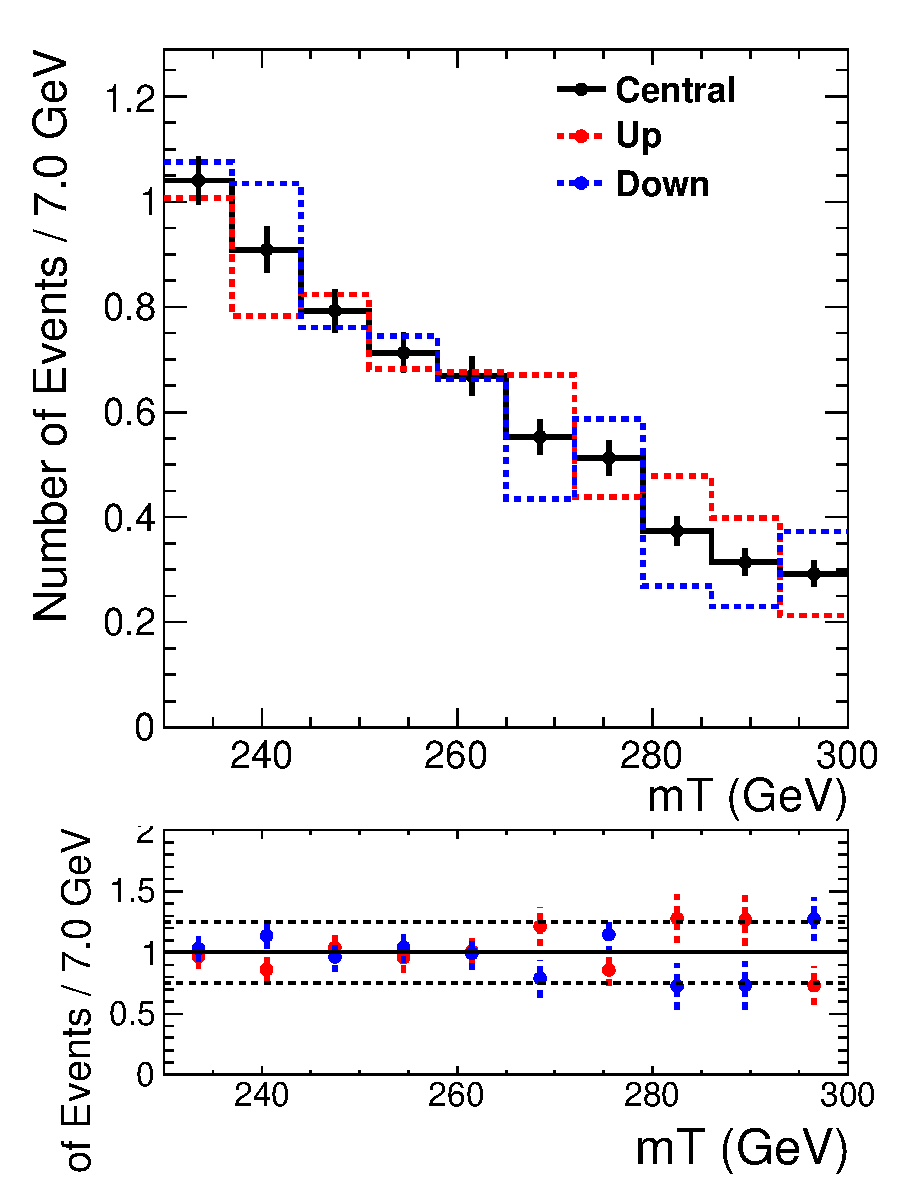
\includegraphics[width=0.49\textwidth]{figures/WZ_WZBounding_mT_mH250_ee_lin.pdf}}
\subfigure[]{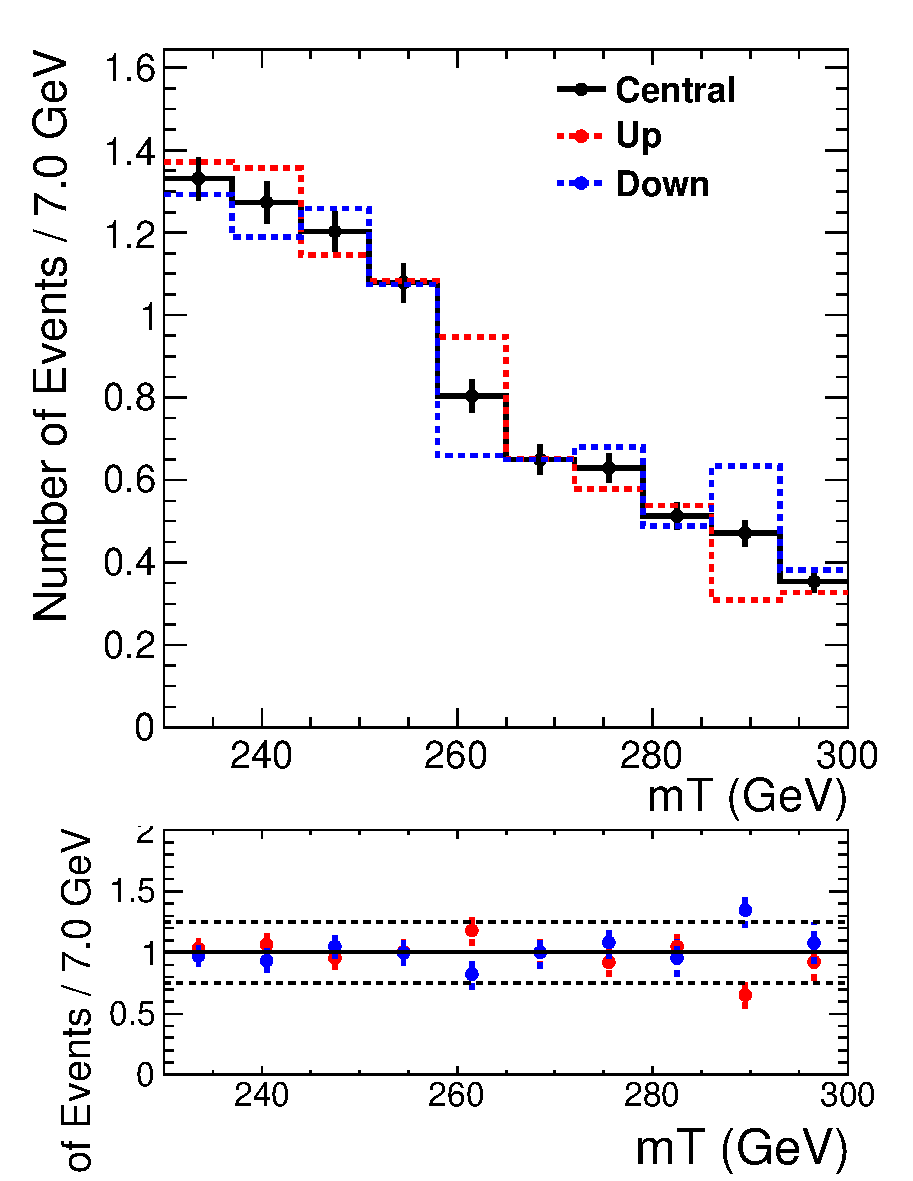
\includegraphics[width=0.49\textwidth]{figures/WZ_WZBounding_mT_mH250_mm_lin.pdf}}\\
\caption{$m_T$ distribution for $\WZ$ for the ee (left) and $\mu\mu$ (right) final states. 
The central shape is taken from pythia with $p_T$ spectrum reweighted to match 
the NLO calcuation. The up histogram is taken from Madgraph with the down 
histogram taken as a variation mirroring the difference between up and central. 
}
\label{fig:wzsyst_hzz}
\end{center}
\end{figure}
%%%%%%%%%%%%%%%%%%%%%%%%
\begin{figure}[!htbp]
\begin{center}
\subfigure[]{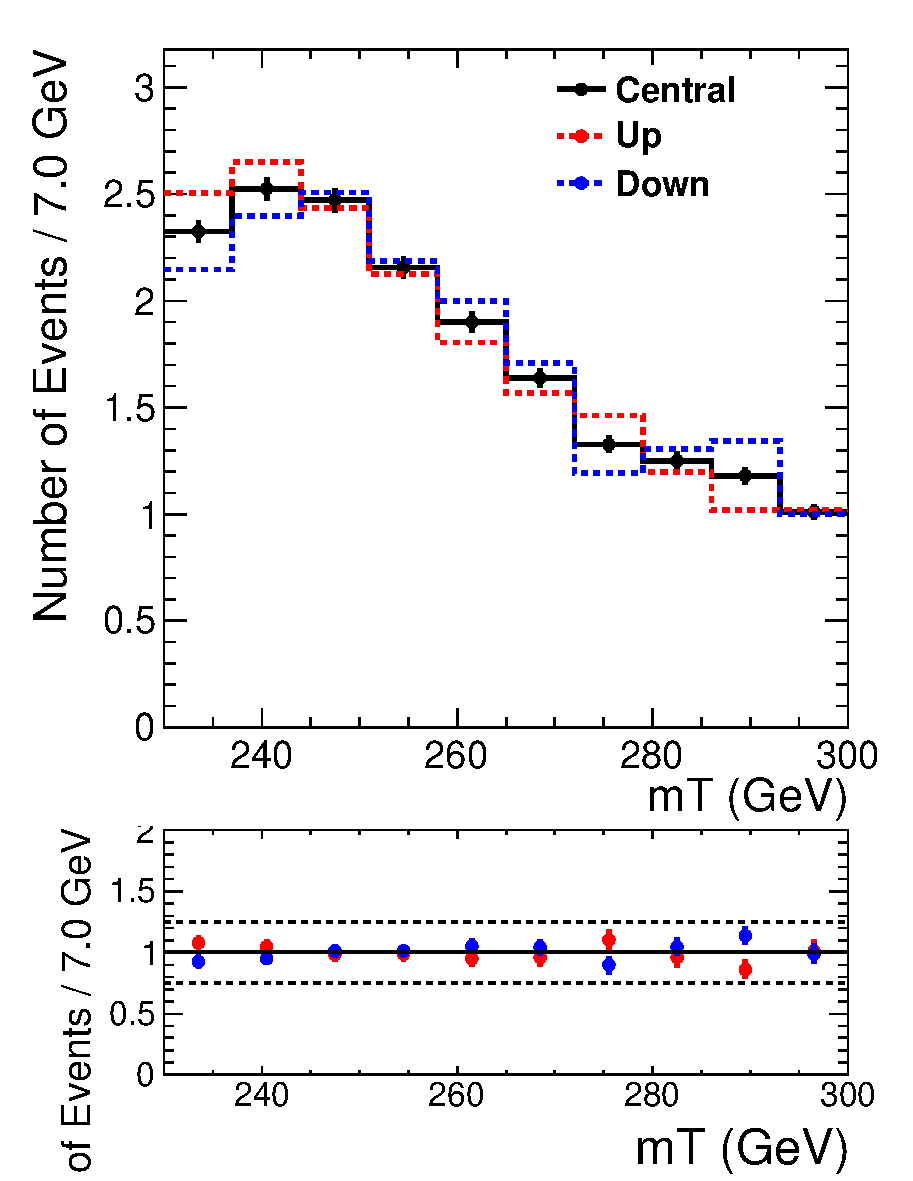
\includegraphics[width=0.49\textwidth]{figures/ZZ_ZZBounding_mT_mH250_ee_lin.pdf}}
\subfigure[]{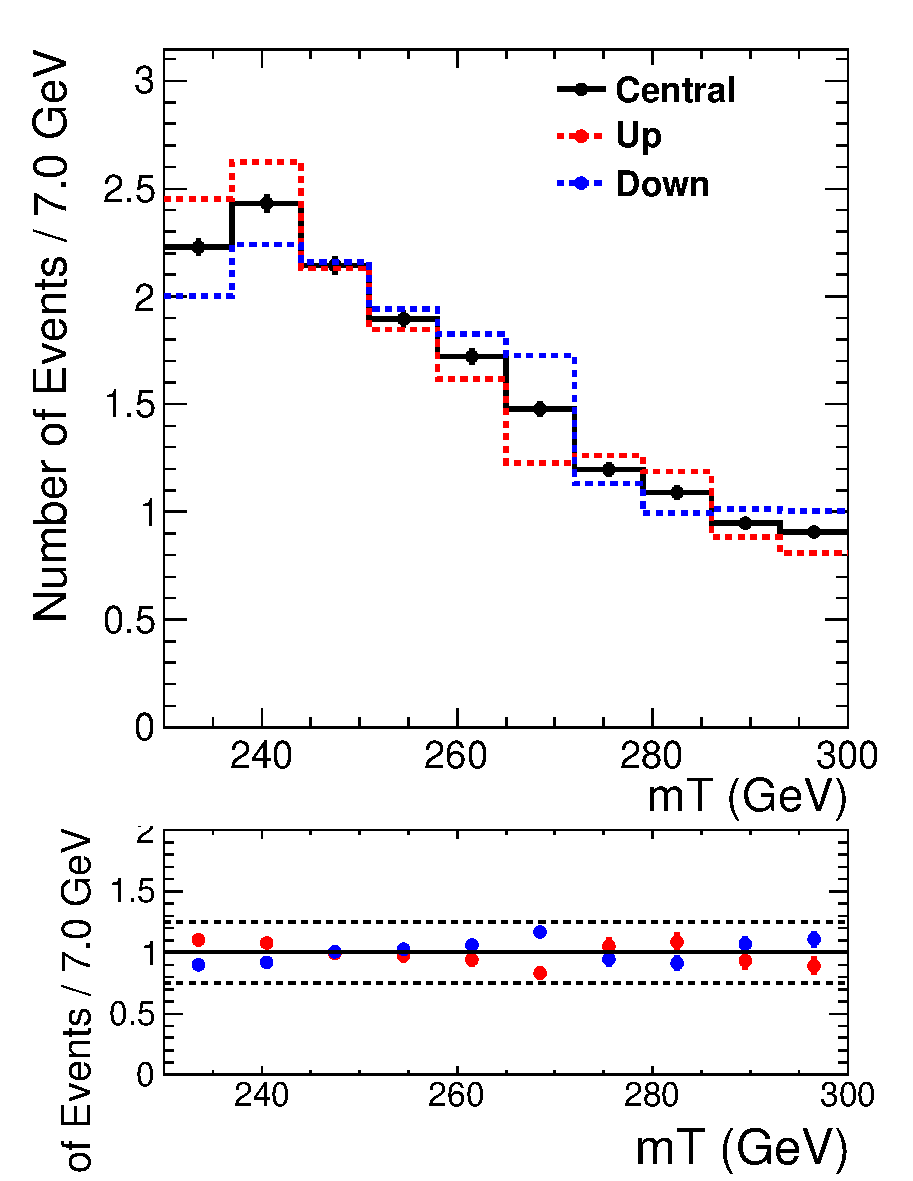
\includegraphics[width=0.49\textwidth]{figures/ZZ_ZZBounding_mT_mH250_mm_lin.pdf}}\\
\caption{$m_T$ distribution for $\ZZ$ for the ee (left) and $\mu\mu$ (right) final states. 
The central shape is taken from pythia with $p_T$ spectrum reweighted to match 
the NLO calcuation. The up histogram is taken from Madgraph with the down 
histogram taken as a variation mirroring the difference between up and central. 
}
\label{fig:zzsyst_hzz}
\end{center}
\end{figure}
%%%%%%%%%%%%%%%%%%%%%%%%


\subsection{Top and \WW\   Background}

For the Top and \WW{} background involving the $\mu^+\mu^-$, $e^+\mu^-$ and 
$e^+e^-$ that occur with equal rates ( after correcting the electron 
to muon efficiency ratio), we can estimate the shapes from data using 
the opposite flavor ($e^\pm\mu^\mp$ states. To ensure the kinematics 
in the opposite flavor states to be the same as in the same flavors, we 
need to apply the same selections in the signal region. The 
statistics is rather limited after the $\met$ preselections and 
b-tagging veto as shown in Fig.~\ref{fig:mtemdatamc}. 

The top background statisitcs can be enriched by relaxing the btag requirement 
in all the dilepton final states. We define this as the control region 
to study the top event shape. Figure~\ref{fig:mtcompsigcontrl} 
compares the $m_T$ distributions between the same flavor signal region and 
the control region and found the two regions give consistent spectrum. 
Figure~\ref{fig:mtdatamcl} shows the comparison of the $m_T$ 
distributions between the signal MC region and the control region in both data and MC. 
Therefore we can use the shapes in the signal regional derived from MC 
as the central shape and place the shapes in the control region derived from Data as the 
alternative, as shown in Figure~\ref{fig:topsyst_hzz} for the $m_H=250\GeVcc$ selection. 

Seperating the top background, the \WW{} background shape variations can be assessed 
in the same way as in the $\hww$ analysis described in the previous section. 
Figure~\ref{fig:wwsyst_hzz}-\ref{fig:wwnlosyst_hzz} show the variations we consider 
for the $m_H=250\GeVcc$ selection. 

%%%%%%%%%%%%%%
\begin{figure}[!htbp]
\begin{center}
\subfigure[]{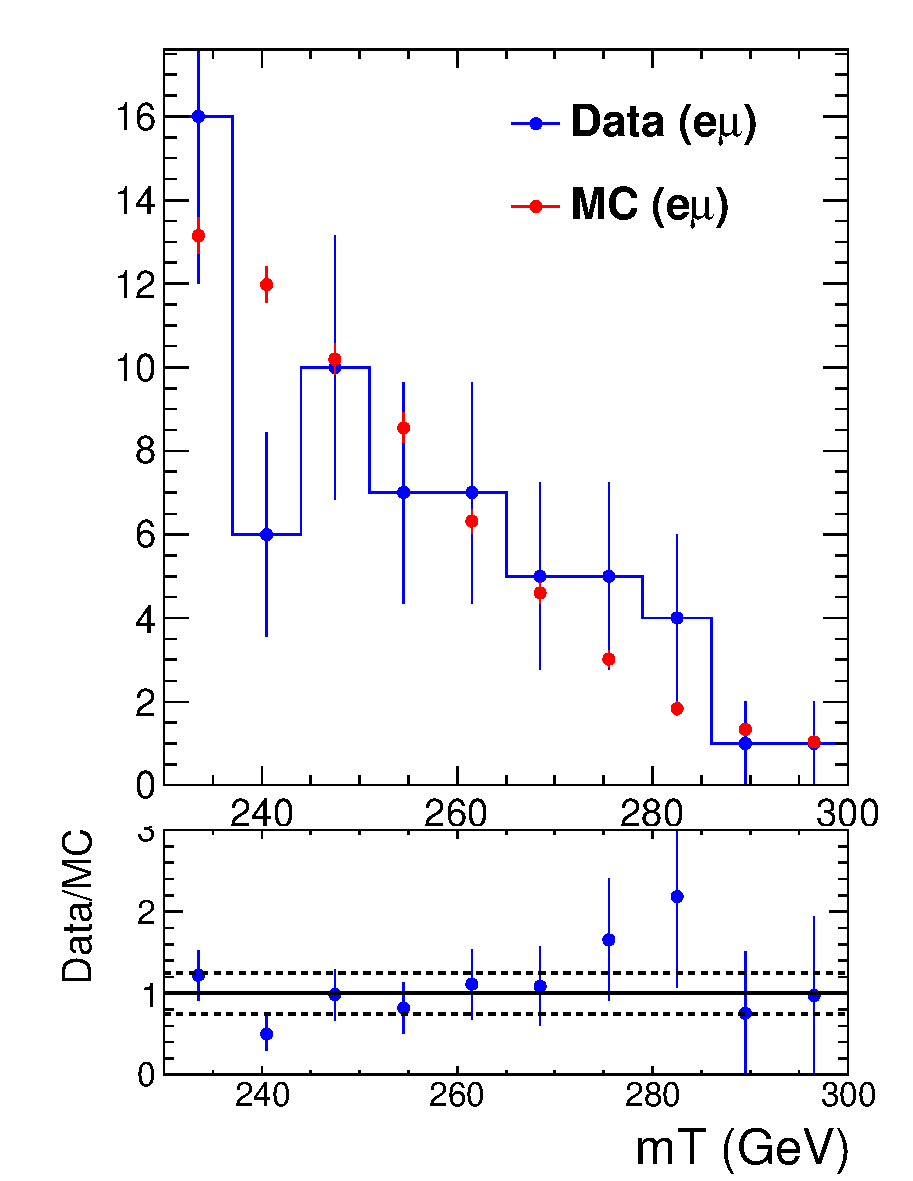
\includegraphics[width=0.49\textwidth]{figures/OF_mT_mH250_datamc_lin.pdf}}\\
\caption{Comparing the $m_T$ transverse mass distribution in the opposite flavor between data and MC.The data corresponds to 1.1/fb.}
\label{fig:mtemdatamc}
\end{center}
\end{figure}
%%%%%%%%%%%%%%

%%%%%%%%%%%%%%
\begin{figure}[!htbp]
\begin{center}
\begin{tabular}{cc}
\subfigure[]{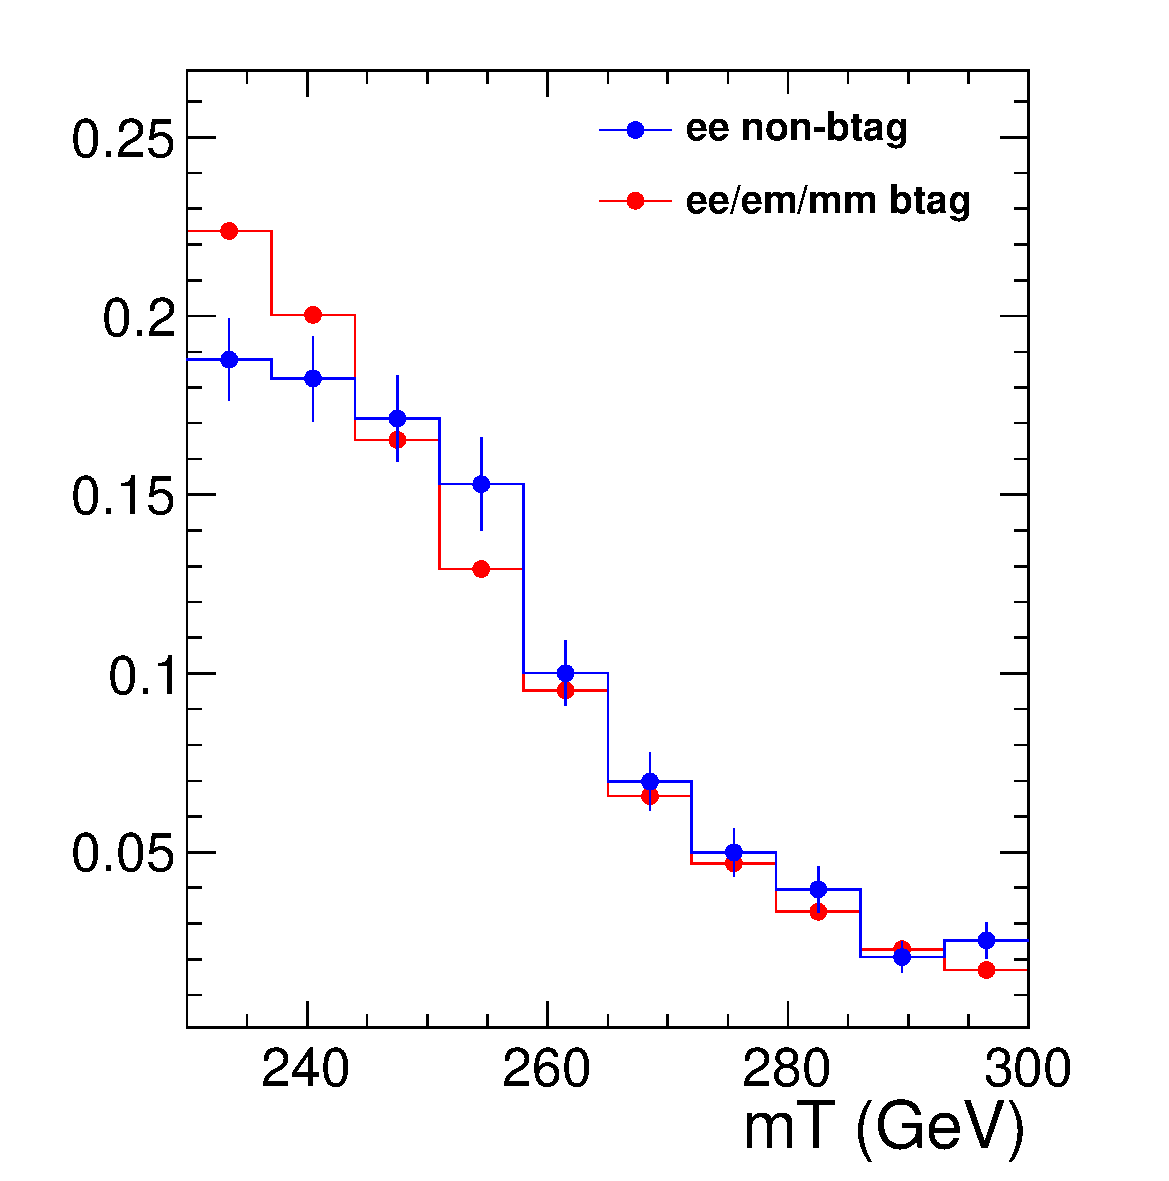
\includegraphics[width=0.49\textwidth]{figures/Top_mT_mH250_ee_lin.pdf}}
\subfigure[]{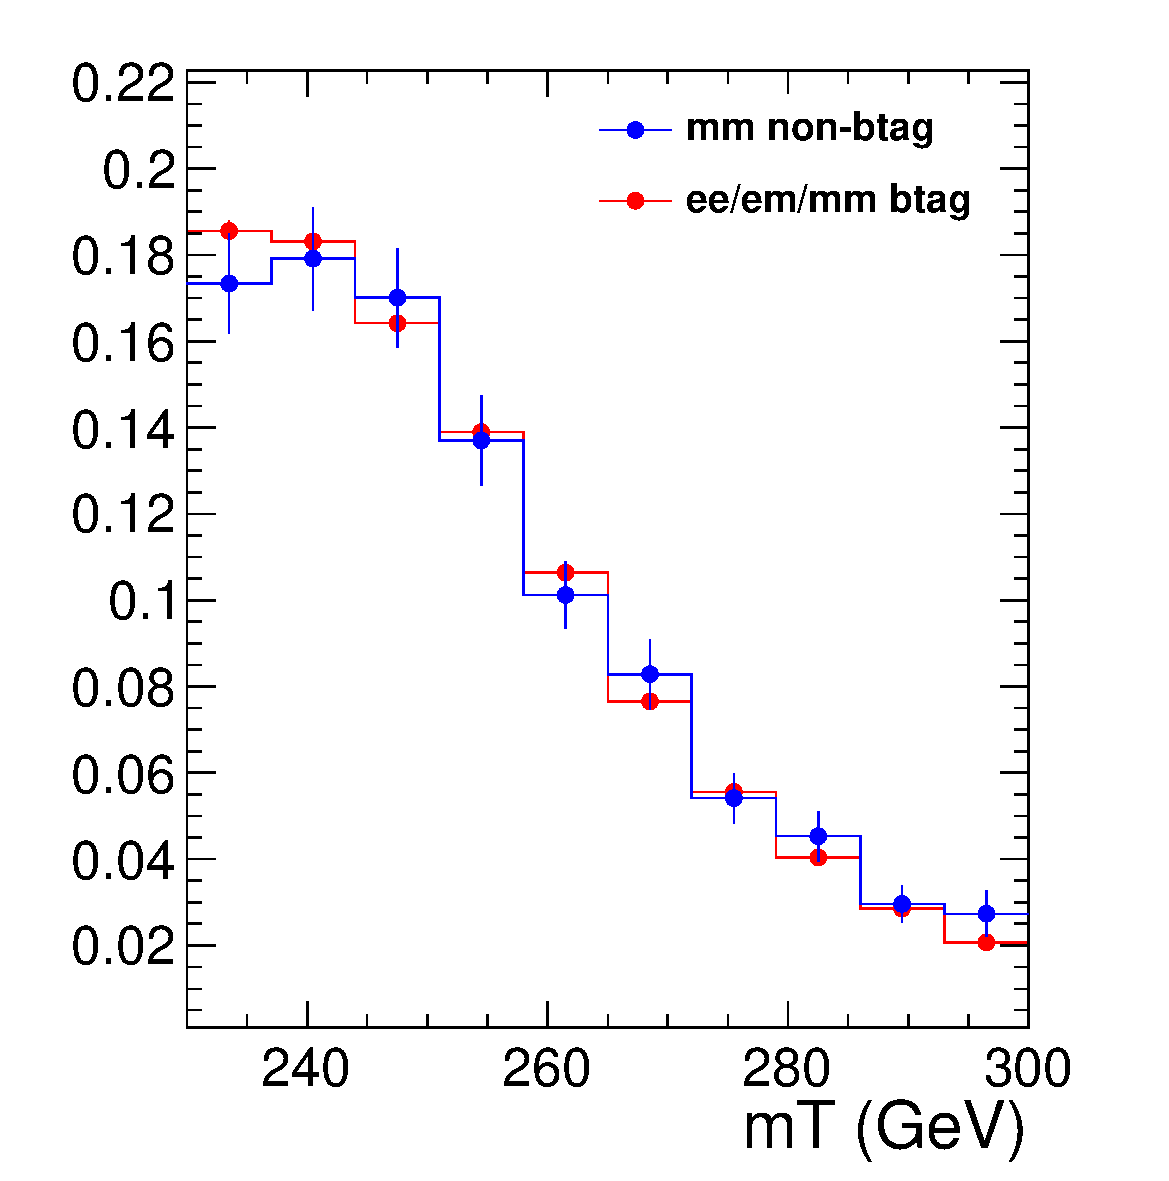
\includegraphics[width=0.49\textwidth]{figures/Top_mT_mH250_mm_lin.pdf}}\\
\end{tabular}
\caption{Comparing the mT distribution in the $H\to ZZ$ signal region and the top enriched control region in $ee/\mu\mu$ final states. This is evaluated with the $mH=250$ selections. }
\label{fig:mtcompsigcontrl}
\end{center}
\end{figure}
%%%%%%%%%%%%%%

%%%%%%%%%%%%%%
\begin{figure}[!htbp]
\begin{center}
\begin{tabular}{cc}
\subfigure[]{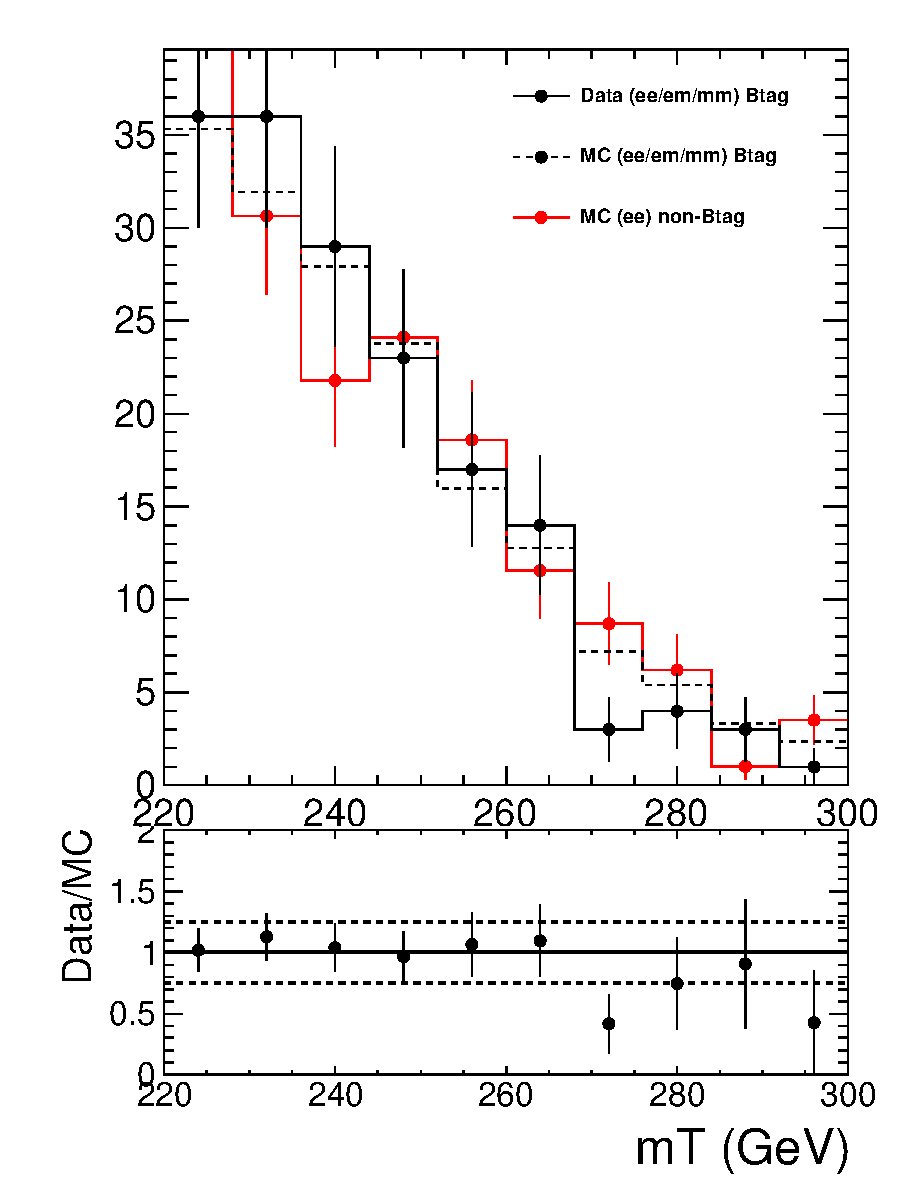
\includegraphics[width=0.49\textwidth]{figures/Top_mT_mH250_datamc_ee_lin.pdf}}
\subfigure[]{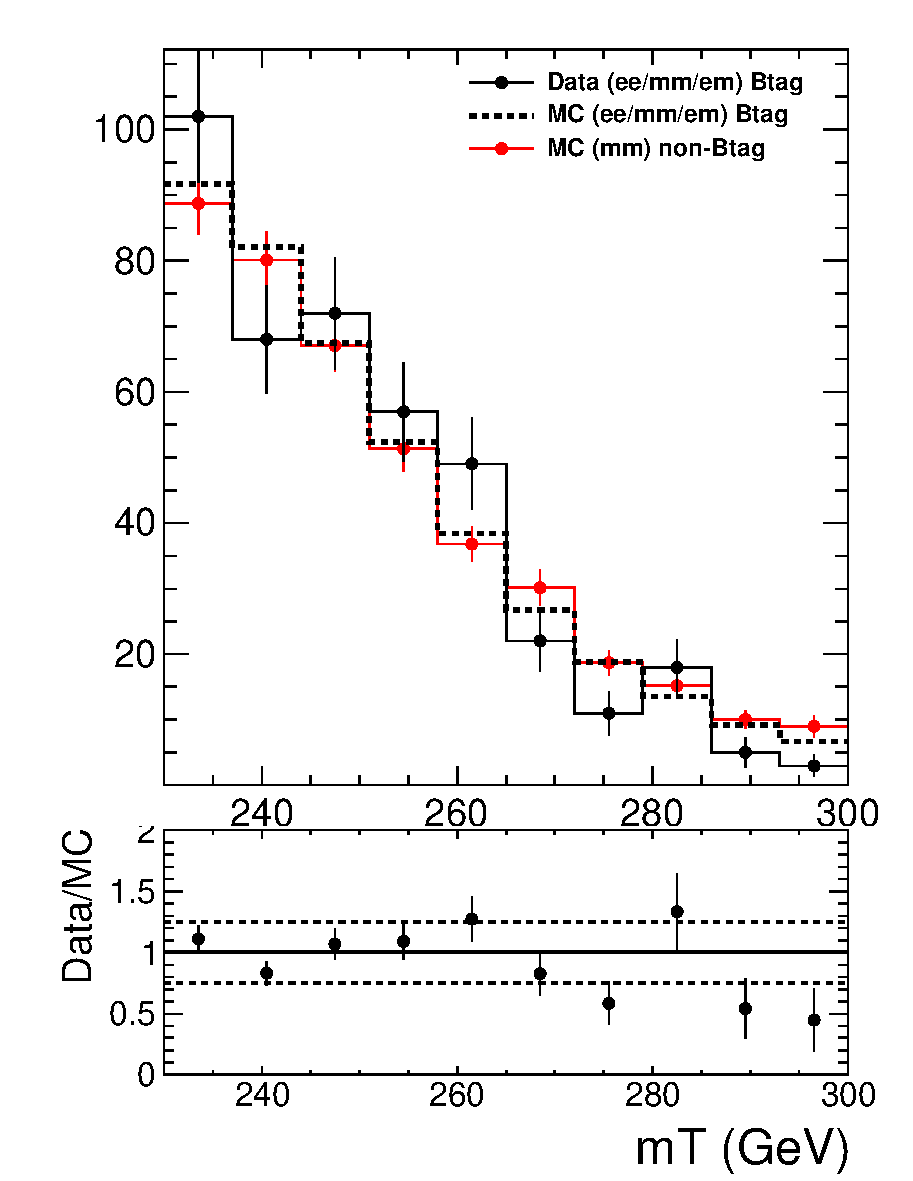
\includegraphics[width=0.49\textwidth]{figures/Top_mT_mH250_datamc_mm_lin.pdf}}\\
\end{tabular}
\caption{Comparing the mT distribution in the $H\to ZZ$ signal region in MC in $ee$ (left) and $\mu\mu$ (right) and the top enriched control region in all dilepton final states requiring btagging. This is evaluated with the $mH=250$ selections. }
\label{fig:mtdatamcl}
\end{center}
\end{figure}
%%%%%%%%%%%%%%



%%%%%%%%%%%%%%%%%%%%%%%%
\begin{figure}[!htbp]
\begin{center}
\subfigure[]{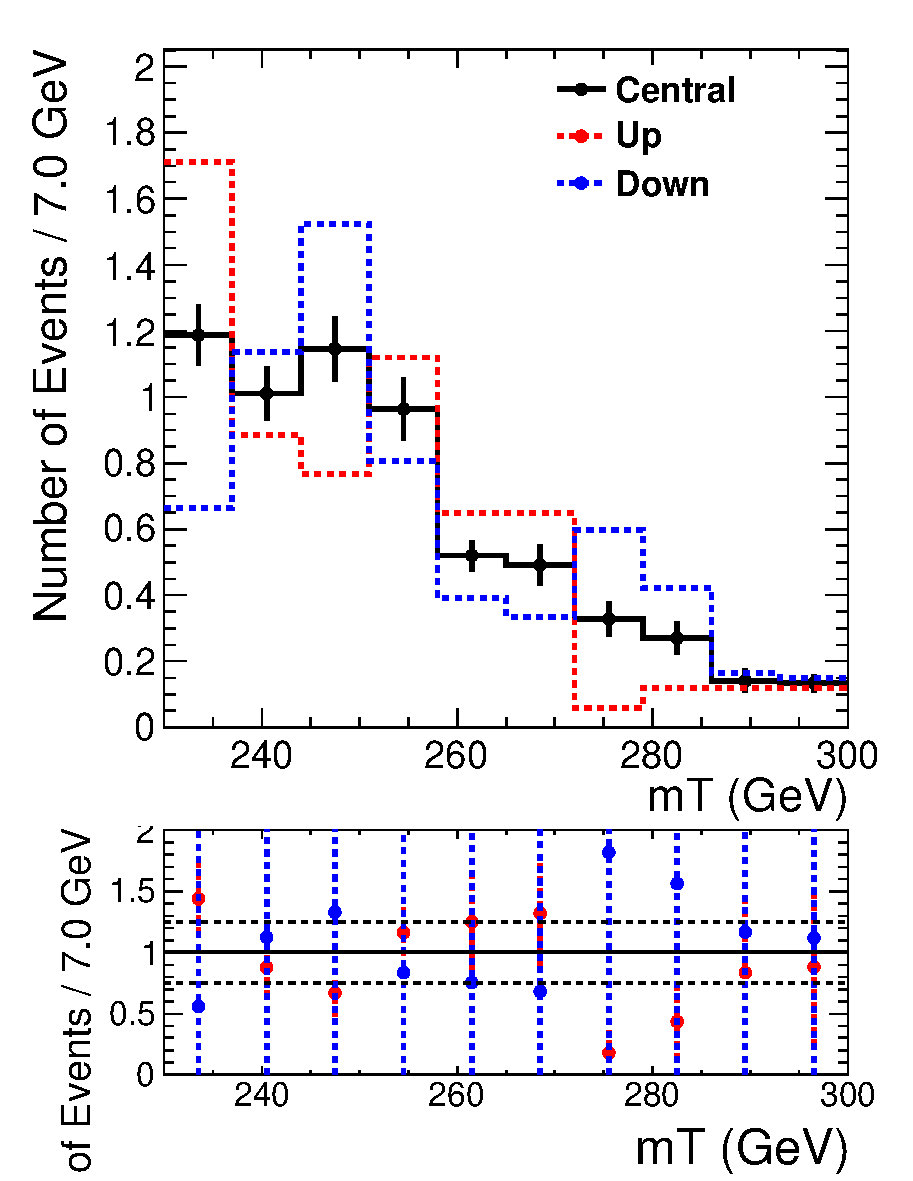
\includegraphics[width=0.49\textwidth]{figures/Top_TopBounding_mT_mH250_ee_lin.pdf}}
\subfigure[]{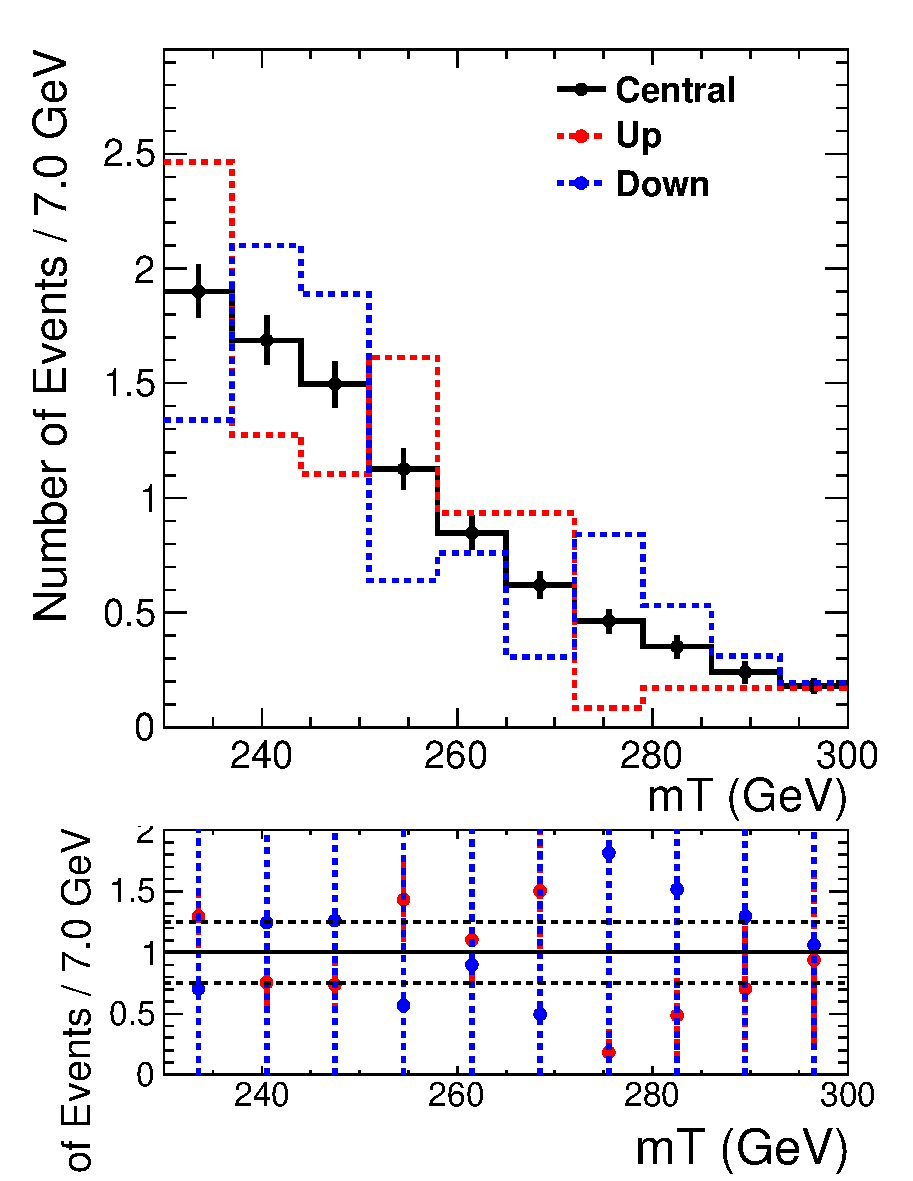
\includegraphics[width=0.49\textwidth]{figures/Top_TopBounding_mT_mH250_mm_lin.pdf}}\\
\caption{$m_T$ distribution for Top for the ee (left) and $\mu\mu$ (right) final states. 
The central shape is taken from MC in the signal region. The up histogram is taken from 
data in the control region, with the down 
histogram taken as a variation mirroring the difference between up and central. 
}
\label{fig:topsyst_hzz}
\end{center}
\end{figure}
%%%%%%%%%%%%%%%%%%%%%%%%

%%%%%%%%%%%%%%%%%%%%%%%%
\begin{figure}[!htbp]
\begin{center}
\subfigure[]{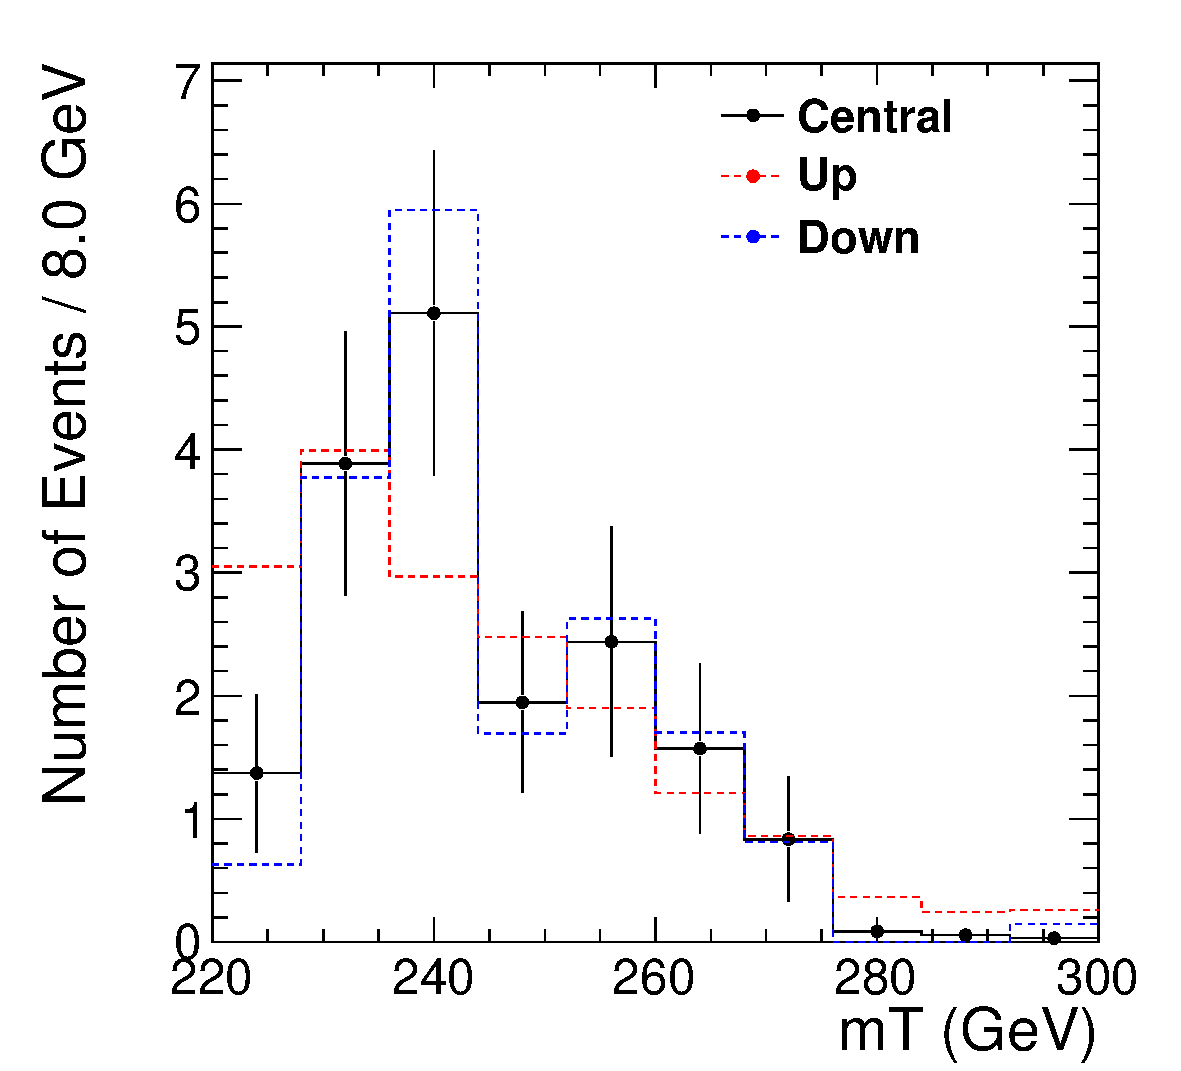
\includegraphics[width=0.49\textwidth]{figures/WW_WWBounding_mT_mH250_ee_lin.pdf}}
\subfigure[]{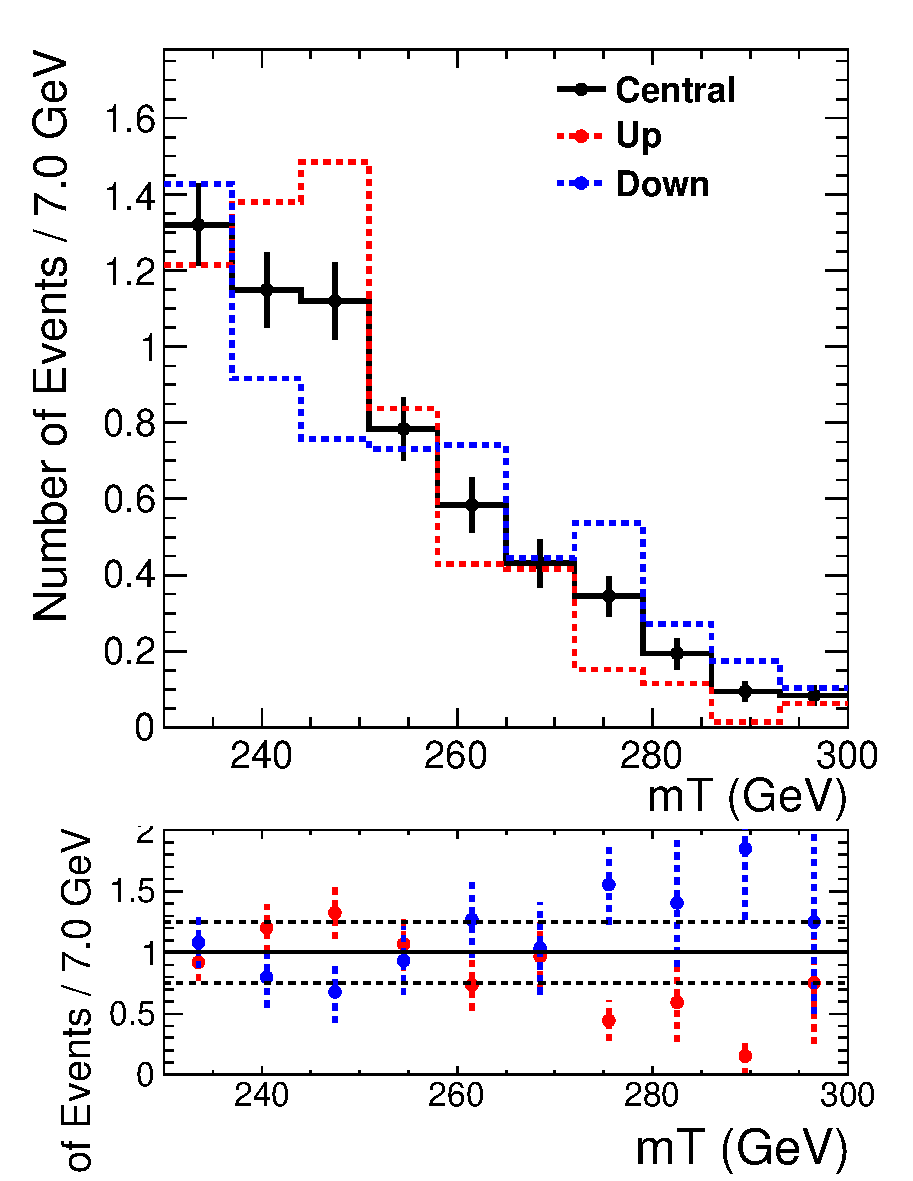
\includegraphics[width=0.49\textwidth]{figures/WW_WWBounding_mT_mH250_mm_lin.pdf}}\\
\caption{$m_T$ distribution for WW for the ee (left) and $\mu\mu$ (right) final states. 
The central shape is taken from Pythia MC. The up histogram is taken from 
MC@NLO, with the down histogram taken as a variation mirroring the difference between up and central. 
}
\label{fig:wwsyst_hzz}
\end{center}
\end{figure}
%%%%%%%%%%%%%%%%%%%%%%%%
%%%%%%%%%%%%%%%%%%%%%%%%
\begin{figure}[!htbp]
\begin{center}
\subfigure[]{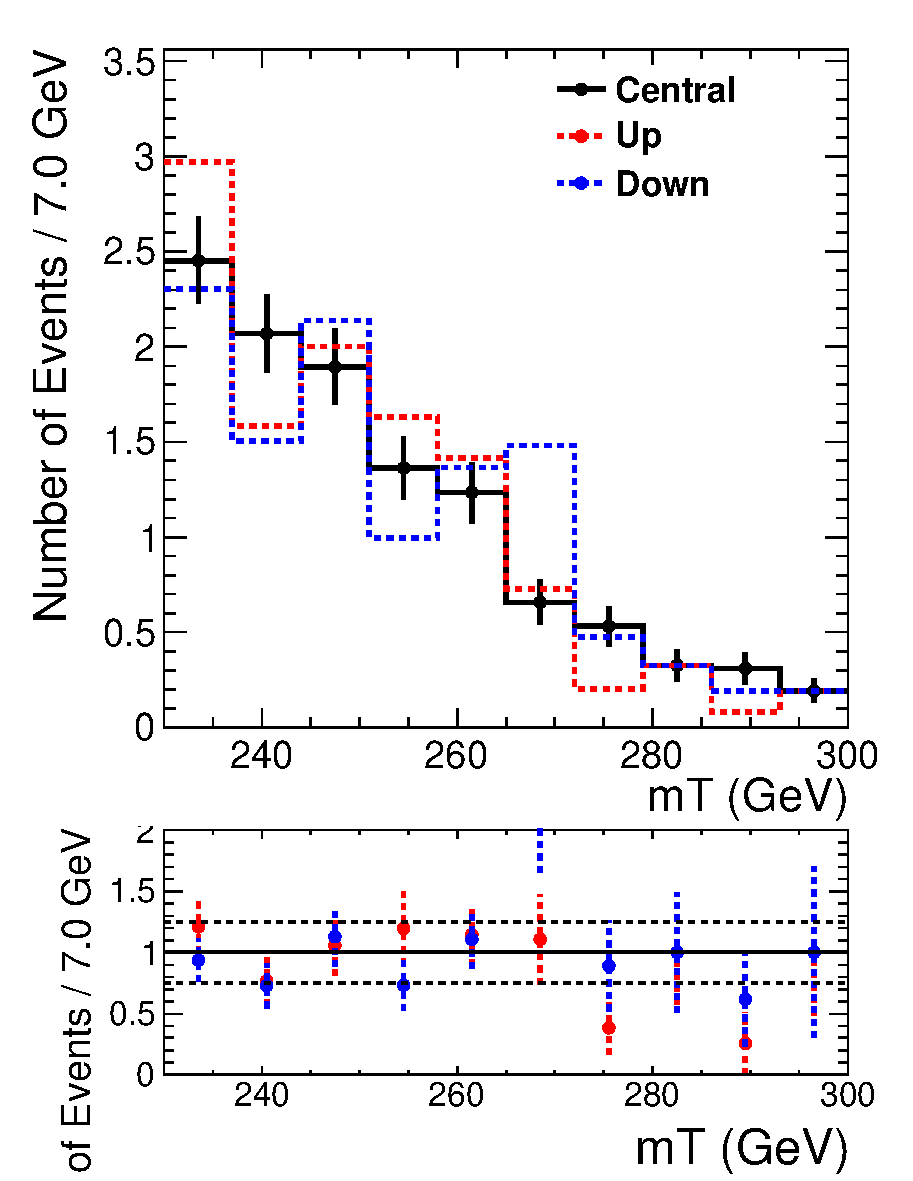
\includegraphics[width=0.49\textwidth]{figures/WW_WWNLOBounding_mT_mH250_ee_lin.pdf}}
\subfigure[]{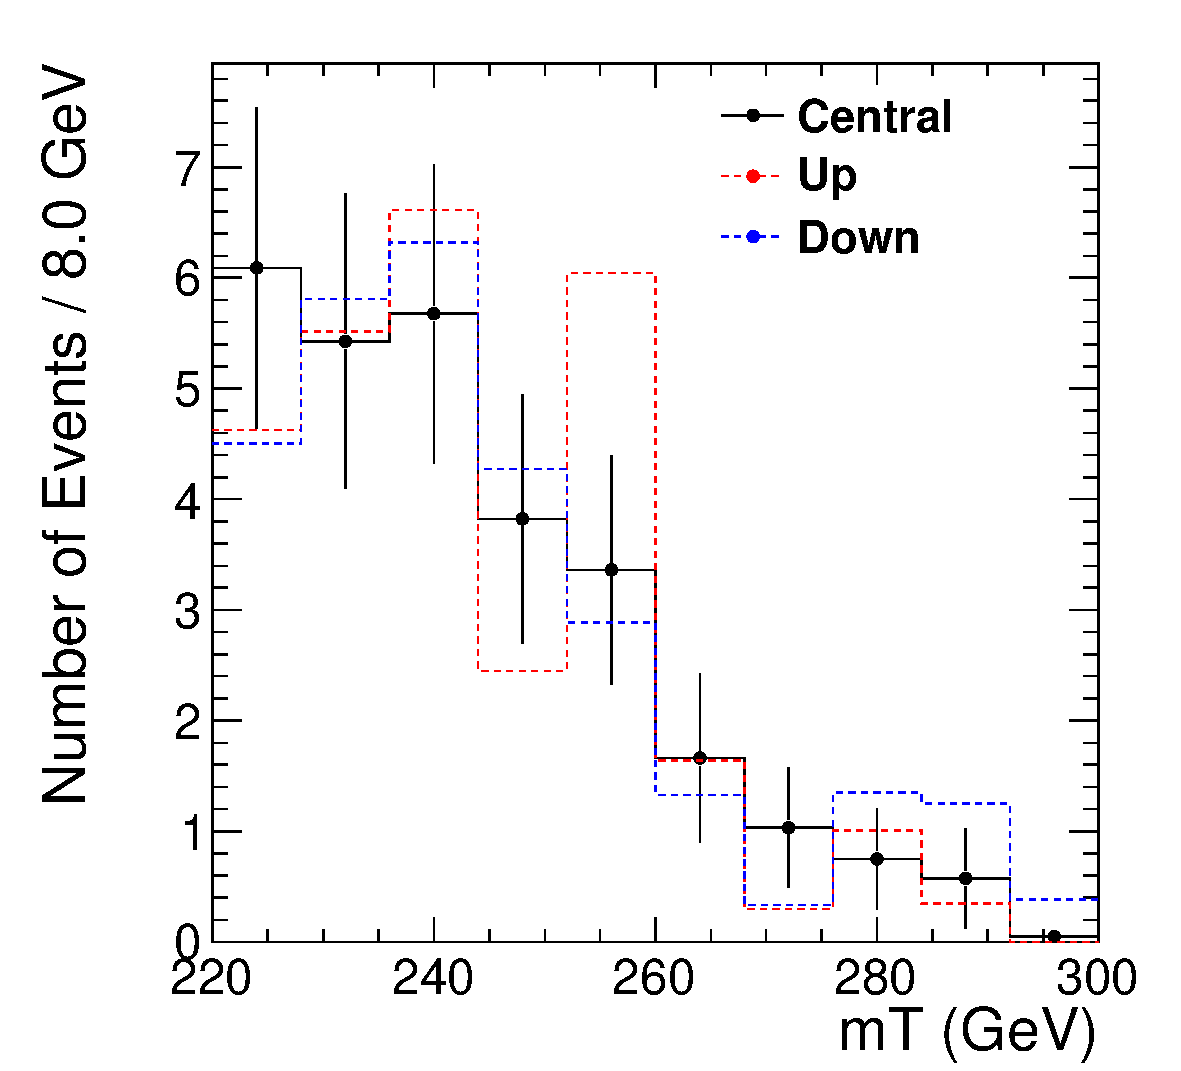
\includegraphics[width=0.49\textwidth]{figures/WW_WWNLOBounding_mT_mH250_mm_lin.pdf}}\\
\caption{$m_T$ distribution for WW for the ee (left) and $\mu\mu$ (right) final states. 
The central shape is taken from Pythia MC. The up/down histogram accounts for the QCD scaling up effect
derived from MC@NLO and scaled to the central shape. 
}
\label{fig:wwnlosyst_hzz}	
\end{center}
\end{figure}
%%%%%%%%%%%%%%%%%%%%%%%%

\subsection{\dyll\  Background}

The \dyll\  background shape can be estimated from data in the $m_T$ and BDT based 
shape analysis. This is because in both method we only use the dilepton momentum 
instead of the individual lepton information as in the matrix element method. 
The intrinsic difference between the photon jet and Z jets events is partially
accounted for in the overal normalization uncertainty. 
The lack of statistics in the \dyll\  background makes the comparison of the 
data-driven shape and the MC shape in the signal region difficult. 
If sufficient MC statistics is available, we can use the shape in the signal region in MC as 
the alternative shape to interpreted as the one sigma variation. 






\subsection{Validation tests}
  \label{sec:validation_zz}
  To validate the procedures discussed in the previous section, detailed studies 
have been carried out using simulated events from the Spring11 CMSSW\_4\_2\_X production.
The basic object selections are taken from the Ref~\cite{hzz}-~\cite{hzzlppas}. 
We evaluate the effects on the expected limits projected to $\mathcal{L}~=~4.0~\pm~0.2~\ifb$. 
The Top and \WW{} background are estimated using data-driven techinques documented in 
Ref.~\cite{hzz}. 
In all the test, we run 10000 toymc to estimate the  effects on the median expected cross-section ration limits and the 1/2-$\sigma$ 
uncertainty bands with a statistical precision about 0.01. 


\subsubsection{Shape vs. Counting Analyses}

As in the $\hww$ analysis, we compare the improvement in the performance using the shape analysis 
with respect to the simple cut-and-cut analysis, shown in 
Table~\ref{tab:mva_mtshapevscuts_hzz}-\ref{tab:mvashape_mevsbdt_hzz}. 

In the $H\to ZZ$ analysis, performing shape analysis based on the $m_T$ variable only 
improves the search sensitivity by about $10-15\%$, ignoring the systematics due to the 
uncertainties of shape variations. 
We have also implemented the preliminary version of the shape analysis 
based on multivariate methods, Matrix Element and the BDT. 
The shape analysis based on the Matrix Element outputs brings additional $X\%$ improvement 
compared to the shape analysis based on $m_T$ for the low higgs mass hypothesis $mH=250\GeVcc$. 
Compared to the shape analysis based on $m_T$, the shape analysis based on the BDT outputs 
brings additional $X\%$ improvement in the intermediate higgs mass hypotheses 
$ 350<=~mH~<=~400\GeVcc$ and additional $X\%$ improvement in the higher mass hypotheses
$mH~>~400\GeVcc$. 

%In the following validations, we use the $m_T$ based shape analysis as an example 
%to demonstrate the effects due to the shape systematics. 

%%%%%%%%%%%%%%%%%%%%%%%%%%%%%
\begin{table}[!ht]
\begin{center}
{\normalsize
\begin{tabular}{|l|c|c|c|c|c|c|}
\hline
      &  \multicolumn{3}{c|}{Cut-and-Count Based Analysis} &\multicolumn{3}{c|}{Shape Analysis using $m_T$} \\
\hline
Mass  &  Median      &     68\% C.L. band &  95\% C.L. band &  Median	   &	 68\% C.L. band &  95\% C.L. band\\
      &  Expected    &                    &                 &  Expected    &			&		 \\
\hline
250 & 1.88 & [1.30, 2.75] & [0.94, 3.86] & 1.62 & [1.14, 2.34] & [0.82, 3.26] \\ 
300 & 1.15 & [0.81, 1.66] & [0.59, 2.31] & 1.00 & [0.71, 1.44] & [0.53, 2.02] \\
350 & 0.77 & [0.54, 1.10] & [0.40, 1.56] & 0.70 & [0.49, 1.00] & [0.37, 1.39] \\
400 & 0.77 & [0.54, 1.08] & [0.39, 1.50] & 0.70 & [0.49, 0.99] & [0.37, 1.37] \\
500 & 1.41 & [0.98, 2.01] & [0.73, 2.87] & 1.26 & [0.90, 1.81] & [0.68, 2.54] \\
600 & 3.12 & [2.18, 4.73] & [1.66, 6.89] & 2.79 & [1.99, 4.03] & [1.53, 5.77] \\
\hline
\end{tabular}
}
\caption{Comparison of the median expected cross section ratio limits as a function 
of the Higgs mass, together with the 1/2-$\sigma$ uncertainty bands between the cut-and-count 
analysis and the shape analysis using the transverse higgs mass. In this comparison, we do not include any systematics due to 
the shape variation. }
\label{tab:mva_mtshapevscuts_hzz}
\end{center}
%\end{table}
%%%%%%%%%%%%%%%%%%%%%%%%%%%%%
%%%%%%%%%%%%%%%%%%%%%%%%%%%%%
%\begin{table}[!ht]
\begin{center}
{\normalsize
\begin{tabular}{|l|c|c|c|c|c|c|}
\hline
      &  \multicolumn{3}{c|}{Shape Analysis using Matrix Element} &\multicolumn{3}{c|}{Shape Analysis using BDT} \\
\hline
Mass  &  Median      &     68\% C.L. band &  95\% C.L. band &  Median	   &	 68\% C.L. band &  95\% C.L. band\\
      &  Expected    &                    &                 &  Expected    &			&		 \\
\hline
250 & 1.19 & [0.84, 1.69] & [0.63, 2.34] & 1.62 & [1.17, 2.35] & [0.87, 3.09] \\
300 & 0.89 & [0.63, 1.25] & [0.46, 1.75] & 0.80 & [0.57, 1.16] & [0.42, 1.56] \\
350 & 0.65 & [0.46, 0.93] & [0.34, 1.31] & 0.45 & [0.32, 0.64] & [0.24, 0.92] \\
400 & 0.64 & [0.46, 0.92] & [0.34, 1.27] & 0.43 & [0.31, 0.62] & [0.23, 0.87]\\
500 & 1.08 & [0.78, 1.52] & [0.58, 2.13] & 0.82 & [0.59, 1.14] & [0.46, 1.67] \\
600 & 2.16 & [1.56, 3.07] & [1.18, 4.31] & 1.88 & [1.37, 2.69] & [1.04, 3.74]\\
\hline
\end{tabular}
}
\caption{\fixme {\bf still use the 5/fb based on 41XMC} 
Comparison of the median expected cross section ratio limits as a function 
of the Higgs mass, together with the 1/2-$\sigma$ uncertainty bands between the cut-and-count 
analysis and the shape analysis using the transverse higgs mass. 
In this comparison, we do not include any systematics due to the shape variation. }
\label{tab:mvashape_mevsbdt_hzz}
\end{center}
\end{table}
%%%%%%%%%%%%%%%%%%%%%%%%%%%%%

\subsubsection{Inclusion of Shape Uncertainties}

In this section, we document the shape systematics effects to the median expected cross section 
ratio limits as a function of the Higgs mass, together with the 1/2-$\sigma$ uncertainty bands. 
The results are based on the shape analysis using $m_T$ variable. 
The following systematic variations are considered,
%%%%%%%%%%%%%%%%%%%%%%%%%%%%%
\begin{itemize}
\item {Statistic uncertainties in the template}
\item {QCD scale variations to the Higgs process}
\item {Top shape variations}
\item {WW shape variations}
\item {WZ shape variations}
\item {ZZ shape variations}.
\end{itemize}
%%%%%%%%%%%%%%%%%%%%%%%%%%%%%
The effects due to the lepton efficiency and scale variations are neglible and we assign only 
the normalization uncertainties. 

Table~\ref{tab:mva_mtshapewithwithout_hzz} shows the effect on the results by including such uncertainties. 
Including the systematics for shape variations, we see the performance degrade by up to 6\% compared 
to the results obtained without shape systematics. 
The effects are larger for the low Higgs mass hypothesis due to the larger uncertainties due to the 
statistical variations in the templates and the Top shape variations. 
Table~\ref{tab:mva_mtshapevscuts_withshapevar_hzz} compares the cut-based results and the one using 
shape analysis including all systematics due to shape variation. 
Overall we see on average about 10\% gain in the performance for most of the 
higgs mass hypothesis. 
To understand the effects of the individual source of the uncertainties, 
we also compare the results by adding each source progressively, shown in Table~\ref{tab:mva_mtshape_detail}. 
Among all the shape systematics, the statistical uncertainty on the template is the leading effect. 



%%%%%%%%%%%%%%%%%%%%%%%%%%%%%
\begin{table}[!ht]
\begin{center}
{\normalsize
\begin{tabular}{|l|c|c|c|c|c|c|}
\hline
      &  \multicolumn{3}{c|}{ without shape uncertainty} &\multicolumn{3}{c|}{ with shape uncertainty} \\
\hline
Mass  &  Median      &     68\% C.L. band &  95\% C.L. band &  Median	   &	 68\% C.L. band &  95\% C.L. band\\
      &  Expected    &                    &                 &  Expected    &			&		 \\
\hline
250 & 1.62 & [1.14, 2.34] & [0.82, 3.26] & 1.71 & [1.19, 2.51] & [0.86, 3.58] \\
300 & 1.00 & [0.71, 1.44] & [0.53, 2.02] & 1.06 & [0.74, 1.51] & [0.53, 2.14] \\
350 & 0.70 & [0.49, 1.00] & [0.37, 1.39] & 0.72 & [0.51, 1.04] & [0.38, 1.47] \\
400 & 0.70 & [0.49, 0.99] & [0.37, 1.37] & 0.71 & [0.50, 1.01] & [0.38, 1.41] \\
500 & 1.26 & [0.90, 1.81] & [0.68, 2.54] & 1.30 & [0.92, 1.88] & [0.69, 2.65] \\
600 & 2.79 & [1.99, 4.03] & [1.53, 5.77] & 2.87 & [2.02, 4.22] & [1.54, 6.09] \\
\hline
\end{tabular}
}
\caption{Comparison of the median expected cross section ratio limits together with the 1/2-$\sigma$ uncertainty bands of 
the shape analysis with and without accounting for the systematics due to the shape variation. 
The results are presented as a function of the Higgs mass. }
\label{tab:mva_mtshapewithwithout_hzz}
\end{center}
%\end{table}
%%%%%%%%%%%%%%%%%%%%%%%%%%%%%
%%%%%%%%%%%%%%%%%%%%%%%%%%%%%
%\begin{table}[!ht]
\begin{center}
{\normalsize
\begin{tabular}{|l|c|c|c|c|c|c|}
\hline
      &  \multicolumn{3}{c|}{Cut-and-Count Based Analysis} &\multicolumn{3}{c|}{Shape Analysis using $m_T$} \\
\hline
Mass  &  Median      &     68\% C.L. band &  95\% C.L. band &  Median	   &	 68\% C.L. band &  95\% C.L. band\\
      &  Expected    &                    &                 &  Expected    &			&		 \\
\hline
250 & 1.88 & [1.30, 2.75] & [0.94, 3.86] & 1.71 & [1.19, 2.51] & [0.86, 3.58] \\
300 & 1.15 & [0.81, 1.66] & [0.59, 2.31] & 1.06 & [0.74, 1.51] & [0.53, 2.14] \\
350 & 0.77 & [0.54, 1.10] & [0.40, 1.56] & 0.72 & [0.51, 1.04] & [0.38, 1.47] \\
400 & 0.77 & [0.54, 1.08] & [0.39, 1.50] & 0.71 & [0.50, 1.01] & [0.38, 1.41] \\
500 & 1.41 & [0.98, 2.01] & [0.73, 2.87] & 1.30 & [0.92, 1.88] & [0.69, 2.65] \\ 
600 & 3.12 & [2.18, 4.73] & [1.66, 6.89] & 2.87 & [2.02, 4.22] & [1.54, 6.09] \\
\hline
\end{tabular}
}
\caption{Comparison of the median expected cross section ratio limits as a function 
of the Higgs mass, together with the 1/2-$\sigma$ uncertainty bands between the cut-and-count 
analysis and the shape analysis using the transverse higgs mass. In this comparison, we include all systematics due to 
the shape variation. }
\label{tab:mva_mtshapevscuts_withshapevar_hzz}
\end{center}
\end{table}
%%%%%%%%%%%%%%%%%%%%%%%%%%%%%
%%%%%%%%%%%%%%%%%%%%%%%%%%%%%
\begin{table}[!ht]
\begin{center}
{\normalsize
\begin{tabular}{|l|c|cccccc|}
\hline
      &  Analysis    & adding          &  adding      &  adding      &  adding      & adding      & adding \\
mH  &  without     & template        &  $H\to ZZ$   &  Top         &  WW          & WZ          & ZZ \\
      &  shape syst. & stat. uncert.   &  QCD effect &  shape syst. &  shape syst. & shape syst. & shape syst. \\
\hline
250 & 1.62 & 1.71 & 1.69 & 1.70 & 1.73 & 1.72 & 1.71 \\   
300 & 1.00 & 1.03 & 1.02 & 1.06 & 1.05 & 1.06 & 1.06 \\ 
350 & 0.70 & 0.71 & 0.71 & 0.72 & 0.72 & 0.72 & 0.72 \\
400 & 0.70 & 0.70 & 0.70 & 0.70 & 0.70 & 0.71 & 0.71 \\
500 & 1.26 & 1.28 & 1.28 & 1.28 & 1.29 & 1.29 & 1.30 \\
600 & 2.79 & 2.88 & 2.84 & 2.84 & 2.86 & 2.88 & 2.87 \\
\hline
\end{tabular}
}
\caption{Comparison of the median expected cross section ratio limits as a function 
of the Higgs mass between shape analysis without and with accouting for the 
shape variation systematics. The results on the various sources are added sequentially 
to study the impact of each source. Note that the statistical precision on the limits 
here are around 1\%. }
\label{tab:mva_mtshape_detail}
\end{center}
\end{table}
%%%%%%%%%%%%%%%%%%%%%%%%%%%%%

\subsection{Result interpretation}
  \label{sec:results_zz}
  \input{results_zz}

%===================================================================================================
\clearpage

\vspace*{-0.2cm}
\thebibliography{12}

\bibitem{pdg}
 K. Nakamura et al. (Particle Data Group), "Review of particle physics", J. Phys.G37 , 2010.

\bibitem{Higgs1}
F. Englert and R. Brout, "Broken symmetries and the masses of gauge bosons", Phys. Rev. Lett. 13,  1964.

\bibitem{Higgs2}
P. W. Higgs, "Broken symmetry and the mass of gauge vector mesons", Phys. Rev. Lett. 13, 1964.

\bibitem{Higgs3}
Guralnik, G.S. and Hagen, C.R. and Kibble, T.W.B., "Global Conservation Laws and Massless Particles", 
Phys.Rev.Lett. 13, 1964.

\bibitem{dittmar}
M.~Dittmar and H.~K.~Dreiner, Phys.\ Rev.\  D {\bf 55} (1997) 167".

\bibitem{HWW2010}
CMS Collaboration, "Measurement of WW Production and Search for the Higgs Boson in 
pp Collisions at $\sqrt{s}$ = 7 TeV", arXiv:1102.5429

\bibitem{HWW2011AN}
L.~Bauerdick et al, "A Higgs Boson Search in the Fully Leptonic $W^+W^-$ Final State", CMS AN-2011/155

\bibitem{VBTFCrossSectionNote}
J. Alcaraz Maestre, \textit{et al.}, "Updated Measurements of Inclusive W and Z Cross Sections 
at $\sqrt{s}=7$ TeV", CMS AN-2010/264.

\bibitem{ggWWError}
F.~ Stoeckli, "http://indico.cern.ch/getFile.py/access?contribId=0\&resId=1\&materialId=slides\&confId=49009", 
EWK Diboson meeting of March 12 2009.

\bibitem{json}
{\small
/afs/cern.ch/cms/CAF/CMSCOMM/COMM\_DQM/certification/Collisions11/7TeV/Prompt/Cert\_160404-163869\_7TeV\_PromptReco\_Collisions11\_JSON.txt
}

\bibitem{ElIso}
A. Vartak, M. LeBourgeois, V. Sharma, "Lepton Isolation in the CMS Tracker, ECAL and HCAL", CMS AN-2010/106.

\bibitem{PVDA}
W. Erdmann, M. LeBourgeois, B. Mangano, 
https://indico.cern.ch/getFile.py/access?contribId=5\&sessionId=3\&resId=1\&materialId=slides\&confId=127127, 
note in preparation.

\bibitem{NExpHits}
B. Mangano \textit{et al.}, "Improvement in Photon Conversion Rejection Performance Using 
Advanced Tracking Tools", AN-10-283.

\bibitem{fakeLeptonNote1}
S.~Xie, \textit{et al.}", "Study of Data-Driven Methods for Estimation of Fake Lepton Backgrounds", 
CMS AN-2009/120.

\bibitem{fakeLeptonNote2}
W.~Andrews, \textit{et al.}, "Fake Rates for dilepton Analyses", CMS AN-2010/257.

\bibitem{fakeLeptonBkgSpillage1}
 F. Golf, D. Evans, J. Mulmenstadt  \textit{et al.}, ``Expectations for observation of top quark pair production in the dilepton final state with the early CMS data'', CMS AN-2009/050.

\bibitem{dyestnote}
W. Andrews, et al., “A Method to Measure the Contribution of $\dyll$ to a di-lepton+ MET Selection”, CMS AN-2009/023 (2009).

\bibitem{jes}
CMS Collaboration, "Jet Energy Calibration with Photon+Jet Events", PAS JME-09-004.

\bibitem{jetpas}
CMS Collaboration, "Jet Performance in pp Collisions at $\sqrt{s}=7 \rm\ TeV$", PAS JME-10-003.

\bibitem{btag}
CMS collaboration, "Commissioning of b-jet identification with pp collisions at $\sqrt{s}=7~\TeV$, BTV-10-001.

\bibitem{antikt}
Cacciari, Matteo and Salam, Gavin P. and Soyez, Gregory, "The anti-$k_t$ jet clustering 
algorithm", JHEP 04,  2008.

\bibitem{ConversionNote}
W.~Andrews, \textit{et al.}, "Study of photon conversion rejection at CMS", CMS AN-2009/159.

\bibitem{tmva}
A. Hoecker, \textit{et al.}, "TMVA - Toolkit for Multivariate Data Analysis", arXiv:physics/0703039, 2007.

\bibitem{XS}
CMS Generator group, Standard Model Cross Sections for CMS at 7 TeV, 2010.

\bibitem{PDF4LHC}
PDF4LHC Working Group, 
{\tt http://www.hep.ucl.ac.uk/pdf4lhc/PDF4LHCrecom.pdf}

\bibitem{Nadolsky:2008zw}
Nadolsky, Pavel M. and others, "Implications of CTEQ global analysis for 
collider observables", Phys. Rev. D78 2008.

\bibitem{Martin:2009iq}
Martin, A. D. and Stirling, W. J. and Thorne, R. S. and Watt, G., "Parton 
distributions for the LHC, Eur. Phys. J. C63 2009.

\bibitem{Ball:2010de}
Ball, Richard D. and others, "A first unbiased global NLO determination 
of parton distributions and their uncertainties", arXiv 1002.4407.

\bibitem{bayesian}
A. O'Hagan and J.J. Forster, "Bayesian Inference", Kendall's Advanced Theory of Statistics, 
Arnold, London, 2B, 2004.

\bibitem{ref:tagprobe_mit_w}
G. Bauer {\it et. al.}, "Lepton ef?iencies for the inclusive W cross section measurement with 36.1pb$^{-1}$", AN2011/097

\bibitem{ref:tagprobe_snt_top}
W. Andrews {\it et. al.}, "Uncertainties on the Lepton Selection Efficiency for t$t\bar{t}$ Cross Section Analysis", AN2010/274

\bibitem{LHCHiggsCrossSectionWorkingGroup:2011ti}
LHC Higgs Cross Section Working Group, "Handbook of LHC Higgs Cross Sections: 
Inclusive Observables", CERN-2011-002, 2011.

\bibitem{PFMET} 
CMS Collaboration, ``CMS MET Performance in Events Containing Electroweak Bosons from pp Collisions at $\sqrt{s}=7$ TeV'', CMS PAS JME-2010-005 (2010)


\bibitem{trkMET} 
Marco Zanetti, ``MET with PU in $\hww\to2\ell$'', https://indico.cern.ch/conferenceDisplay.py?confId=131580
Benjamin Hooberman, ``MET with PU in MC and First 2011 Data'', https://indico.cern.ch/contributionDisplay.py?contribId=5\&confId=132579. 


\bibitem{lands}
Mingshui Chen and Andrey Korytov, https://mschen.web.cern.ch/mschen/lands/

\bibitem{MCFMHiggsProduction}
J. Campbell, R.K. Ellis, G. Zanderighi, ``Next-to-Leading order Higgs + 2 jet production via gluon fusion.'', JHEP 0610:028 (2006), hep-ph/0608194

\bibitem{MCFMVVProduction}
J. Campbell, R.K. Ellis, C. Williams, ``Vector boson pair production at the LHC.'', arxiv:hep-ph/1105.0020.

\bibitem{MITHggNote} 
G. Bauer et al., ``Higgs Search in the pp $\rightarrow$ H $\rightarrow$ $\gamma\gamma$ channel at $\sqrt{s}=7$ TeV'', CMS AN-2011/168. 



%===================================================================================================
%% \newpage 
%% \appendix
%% \appendixpage
%% \section{Data Samples}
%%   \label{app:datasets}
%%   %UPDATEME%
The datasets used for this analysis are summarized in Tables.~\ref{tab:DatasetsData} 
and~\ref{tab:DatasetsMC} for data and Monte Carlo, respectively. The total integrated
luminosity is 49 $\pm$ 2 $\ipb$. We used just basic quality requirements, since an official good 
run list (JSON file) was not available. It will be used in future updates.
For Monte Carlo simulation we use madgraph when possible, 
but different generators such as Pythia and Powheg 
are also used. 
%For $gg \to \WW$ a dedicated generator is used. For \wz\ and \zz\
%processes we use Pythia, since MadGraph samples are mixed with $\WW$ in
%a single $VV$ sample, which is difficult to use properly.

%The choice of the Monte Carlo samples depends on the sample
%availability, but in general we tried to be consistent and use a
%single generator - MadGraph. In the case of Drell-Yan, MadGraph samples
%are not adequate to cover the full mass spectrum. The main sample has a 50 $\GeVcc$ 
%minimum dilepton mass requirement, while the other one, covering
%the low mass region, has an additional requirement on extra jet
%activity. 
%We use madgraph when possible, but different generators are used for some samples
%For $gg \to \WW$ a dedicated generator is used. For \wz\ and \zz\
%processes we use Pythia, since MadGraph samples are mixed with $\WW$ in
%a single $VV$ sample, which is difficult to use properly.

%UPDATEME%
\begin{table}[!ht]
\begin{center}
\begin{tabular}{|c|c|}
\hline
 Dataset Description                   &   Dataset Name   \\
\hline
\hline
\multicolumn{2}{|c|}{$H \to \WW$ Signal Selection Samples} \\
\hline
Run2011A MuEl PromptReco            &  /MuEG/Run2011A-PromptReco-v*/AOD   \\
Run2011A DiMuon PromptReco          &  /DoubleMu/Run2011A-PromptReco-v*/AOD   \\
Run2011A SingleMuon PromptReco      &  /SingleMu/Run2011A-PromptReco-v*/AOD   \\
Run2011A DiElectron PromptReco      &  /DoubleElectron/Run2011A-PromptReco-v*/AOD   \\
\hline
\hline
\multicolumn{2}{|c|}{Fake Rate Measurement Samples} \\
\hline
Run2010A Jet  PromptReco            & /Jet/Run2011A-PromptReco-v*/AOD	\\
Run2010B Photon PromptReco          & /Photon/Run2011A-PromptReco-v*/AOD \\
\hline
\end{tabular}
\caption{Summary of data datasets used.\label{tab:DatasetsData}}
\end{center}
\end{table}

\begin{table}[!ht]
\begin{center}
{\footnotesize
\begin{tabular}{|c|c|c|}
\hline
\multicolumn{3}{|c|}{With Pileup: Processed dataset name is always} \\
\multicolumn{3}{|c|}{/Spring11-PU\_S1\_START311\_V1G1-v*/AODSIM} \\
\hline
 Dataset Description                     &   Primary Dataset Name   & cross-section (pb)\\
\hline
qq $\rightarrow WW$                  	 &   /VVJetsTo4L\_TuneD6T\_7TeV-madgraph-tauola                        &  43.0  \\
gg $\rightarrow WW \to 2l 2\nu$          &   /GluGluToWWTo4L\_TuneZ2\_7TeV-gg2ww-pythia6                       &   0.153\\
$\ttbar$                              	 &   /TTJets\_TuneZ2\_7TeV-madgraph-tauola                             & 157.5 \\
$\singletops$                  	 	 &   /TToBLNu\_TuneZ2\_s-channel\_7TeV-madgraph                        &  1.4 \\
$\singletopt$                  	 	 &   /TToBLNu\_TuneZ2\_t-channel\_7TeV-madgraph                        &  20.9 \\
tW                                    	 &   /TToBLNu\_TuneZ2\_tW-channel\_7TeV-madgraph                       &  10.6 \\
Z[20-inf] $\rightarrow ee$	  	 &   /DYToEE\_M-20\_CT10\_TuneZ2\_7TeV-powheg-pythia                   &  1666.0 \\
Z[20-inf] $\rightarrow \mu\mu$        	 &   /DYToMuMu\_M-20\_CT10\_TuneZ2\_7TeV-powheg-pythia                 &  1666.0 \\	       
Z[20-inf] $\rightarrow \tau\tau$  	 &   /DYToTauTau\_M-20\_CT10\_TuneZ2\_7TeV-powheg-pythia-tauola        &  1666.0 \\
Z[10-20]  $\rightarrow ee$	  	 &   /DYToEE\_M-10To20\_CT10\_TuneZ2\_7TeV-powheg-pythia               &  3892.9 \\
Z[10-20]  $\rightarrow \mu\mu$    	 &   /DYToMuMu\_M-10To20\_CT10\_TuneZ2\_7TeV-powheg-pythia             &  3892.9 \\
Z[10-20]  $\rightarrow \tau\tau$  	 &   /DYToTauTau\_M-10To20\_CT10\_TuneZ2\_7TeV-powheg-pythia-tauola    &  3892.9 \\
W/Z+$\gamma$                       	 &   /PhotonVJets\_7TeV-madgraph                                       &  165.0 \\
W $\rightarrow$ $\ell\nu$           	 &   /WJetsToLNu\_TuneZ2\_7TeV-madgraph-tauola                         &  31314.0 \\
WZ                               	 &   /WZtoAnything\_TuneZ2\_7TeV-pythia6-tauola                        &  18.2 \\
ZZ                               	 &   /ZZtoAnything\_TuneZ2\_7TeV-pythia6-tauola                        &   5.9\\
$gg \to H \to WW \to 2\ell2\nu$          &   /GluGluToHToWWTo2L2Nu\_M-*\_7TeV-powheg-pythia6                   & vary \\
$gg \to H \to WW \to \ell\tau2\nu$       &   /GluGluToHToWWTo2L2Nu\_M-*\_7TeV-powheg-pythia6                   & vary \\
$gg \to H \to WW \to 2\tau2\nu$          &   /GluGluToHToWWTo2Tau2Nu\_M-*\_7TeV-powheg-pythia6                 & vary \\
$qqH,~H \to WW \to 2\ell2\nu$            &   /VBF\_HToWWTo2L2Nu\_M-*\_7TeV-powheg-pythia6                      & vary \\
$qqH,~ H \to WW \to \ell\tau2\nu$	 &   /VBF\_HToWWTo2Tau2Nu\_M-*\_7TeV-powheg-pythia6                    & vary \\
$qqH,~H \to WW \to 2\tau2\nu$	         &   /VBF\_HToWWToLNuTauNu\_M-*\_7TeV-powheg-pythia6                   & vary \\
$WH/ZH/\ttbar H,~H\to WW$                &   /WH\_ZH\_TTH\_HToWW\_M-*\_7TeV-pythia6                            & vary \\
\hline
\hline
\end{tabular}
}
\caption{Summary of Monte Carlo datasets used.\label{tab:DatasetsMC}. The cross sections for a SM Higgs boson
is taken from the LHC Higgs cross-section working group~\cite{LHCHiggsCrossSectionWorkingGroup:2011ti}}
\end{center}
\end{table}

Due to details in the implementation of the Powheg calculation, the
resulting Higgs $\pt$ spectrum for $gg \to H$ has a much harder
spectrum compared with the most precise spectrum calculated to NNLO
with resummation to NNLL order, as illustrated in
Figure~\ref{fig:h160ww_pthiggs}(a). Therefore, the proper procedure is
to apply an event-by-event rewighting to the Powheg simulated
events. For the time being we correct the $gg \to H \to \WW$ jet bin
efficiency computed from the Powheg Monte Carlo sample, by a scale
factor which is approximately identical for all Higgs masses. The
scale factors applied to each jet bin in the Powheg simulation are
shown in Figure~\ref{fig:h160ww_pthiggs}(b). The jet definition is 
consitent with the one used in the analysis.

\begin{figure}[!htbp]
\begin{center}
   \subfigure[]{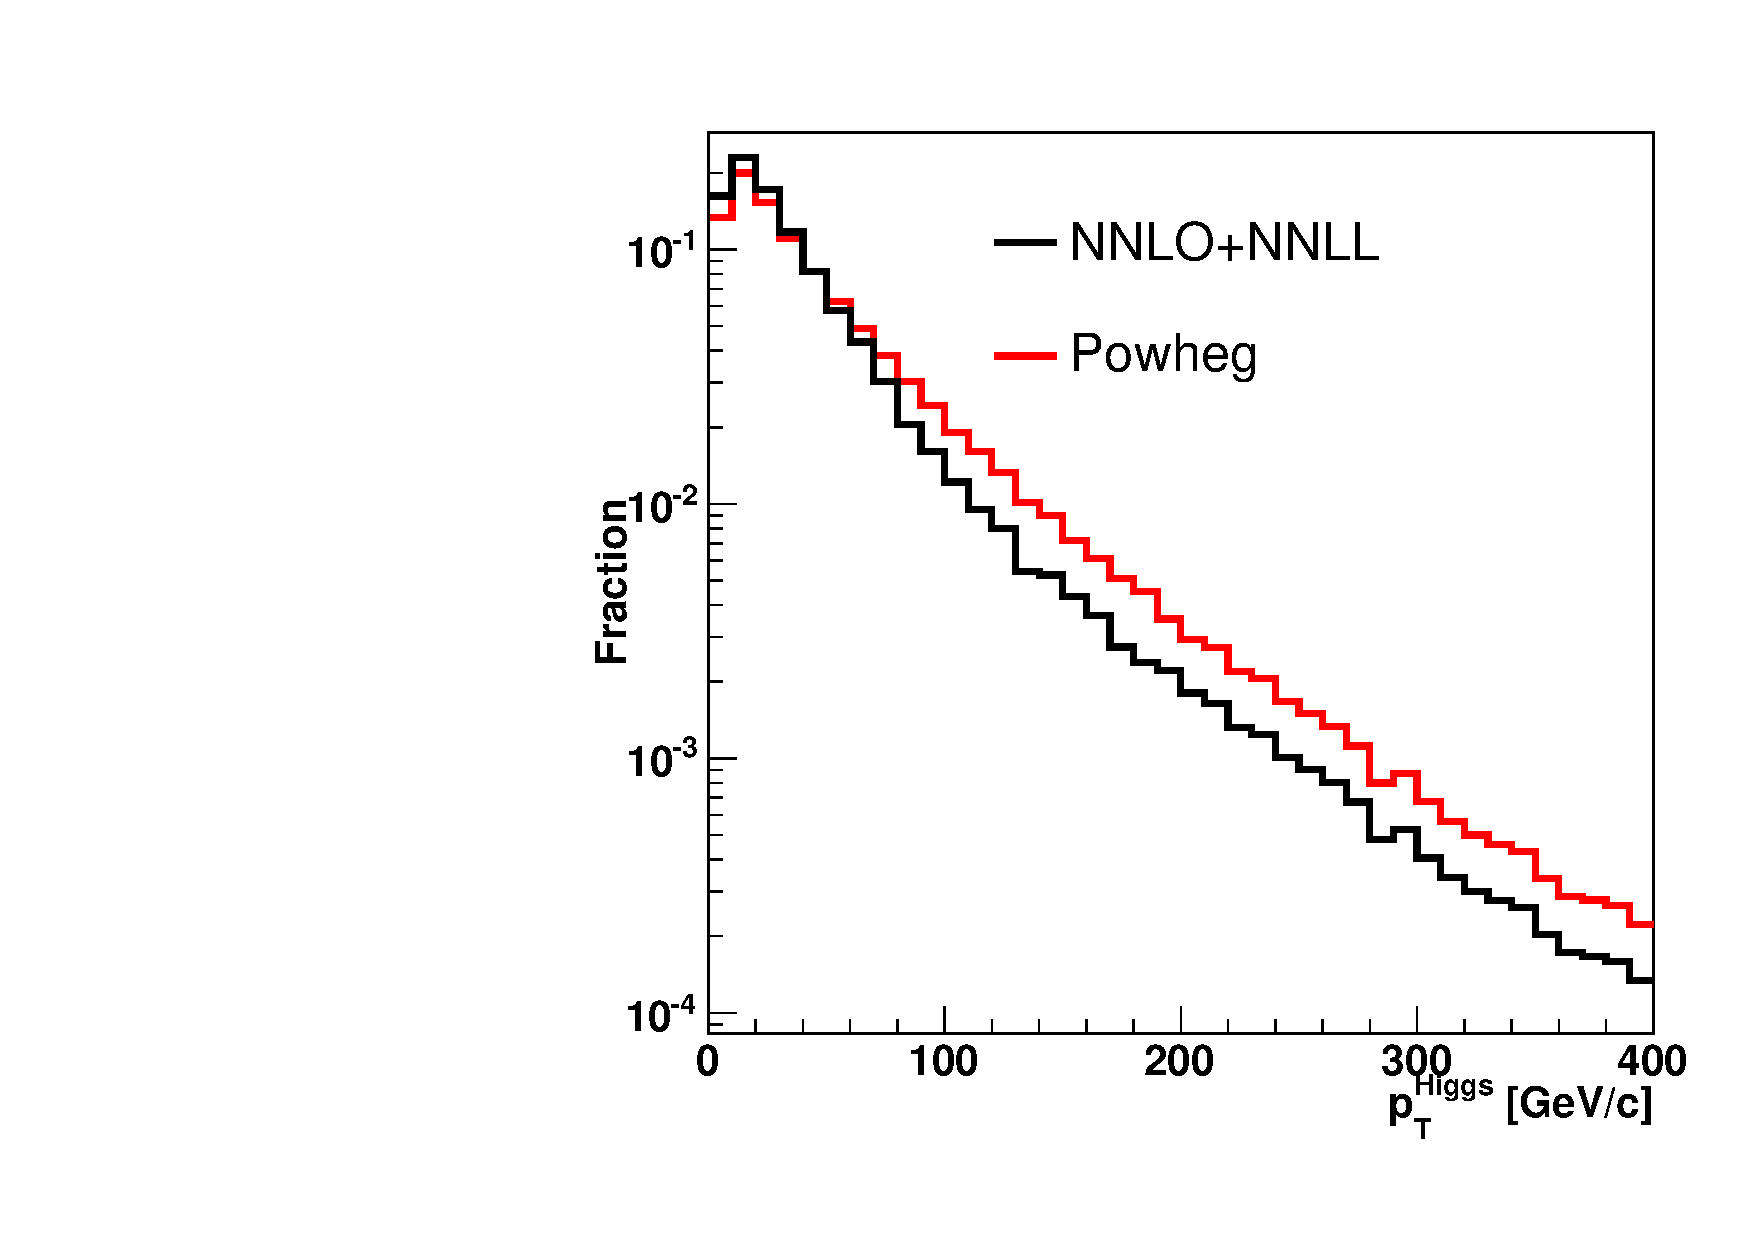
\includegraphics[width=0.49\textwidth]{figures/h160ww_pthiggs.pdf}}
   \subfigure[]{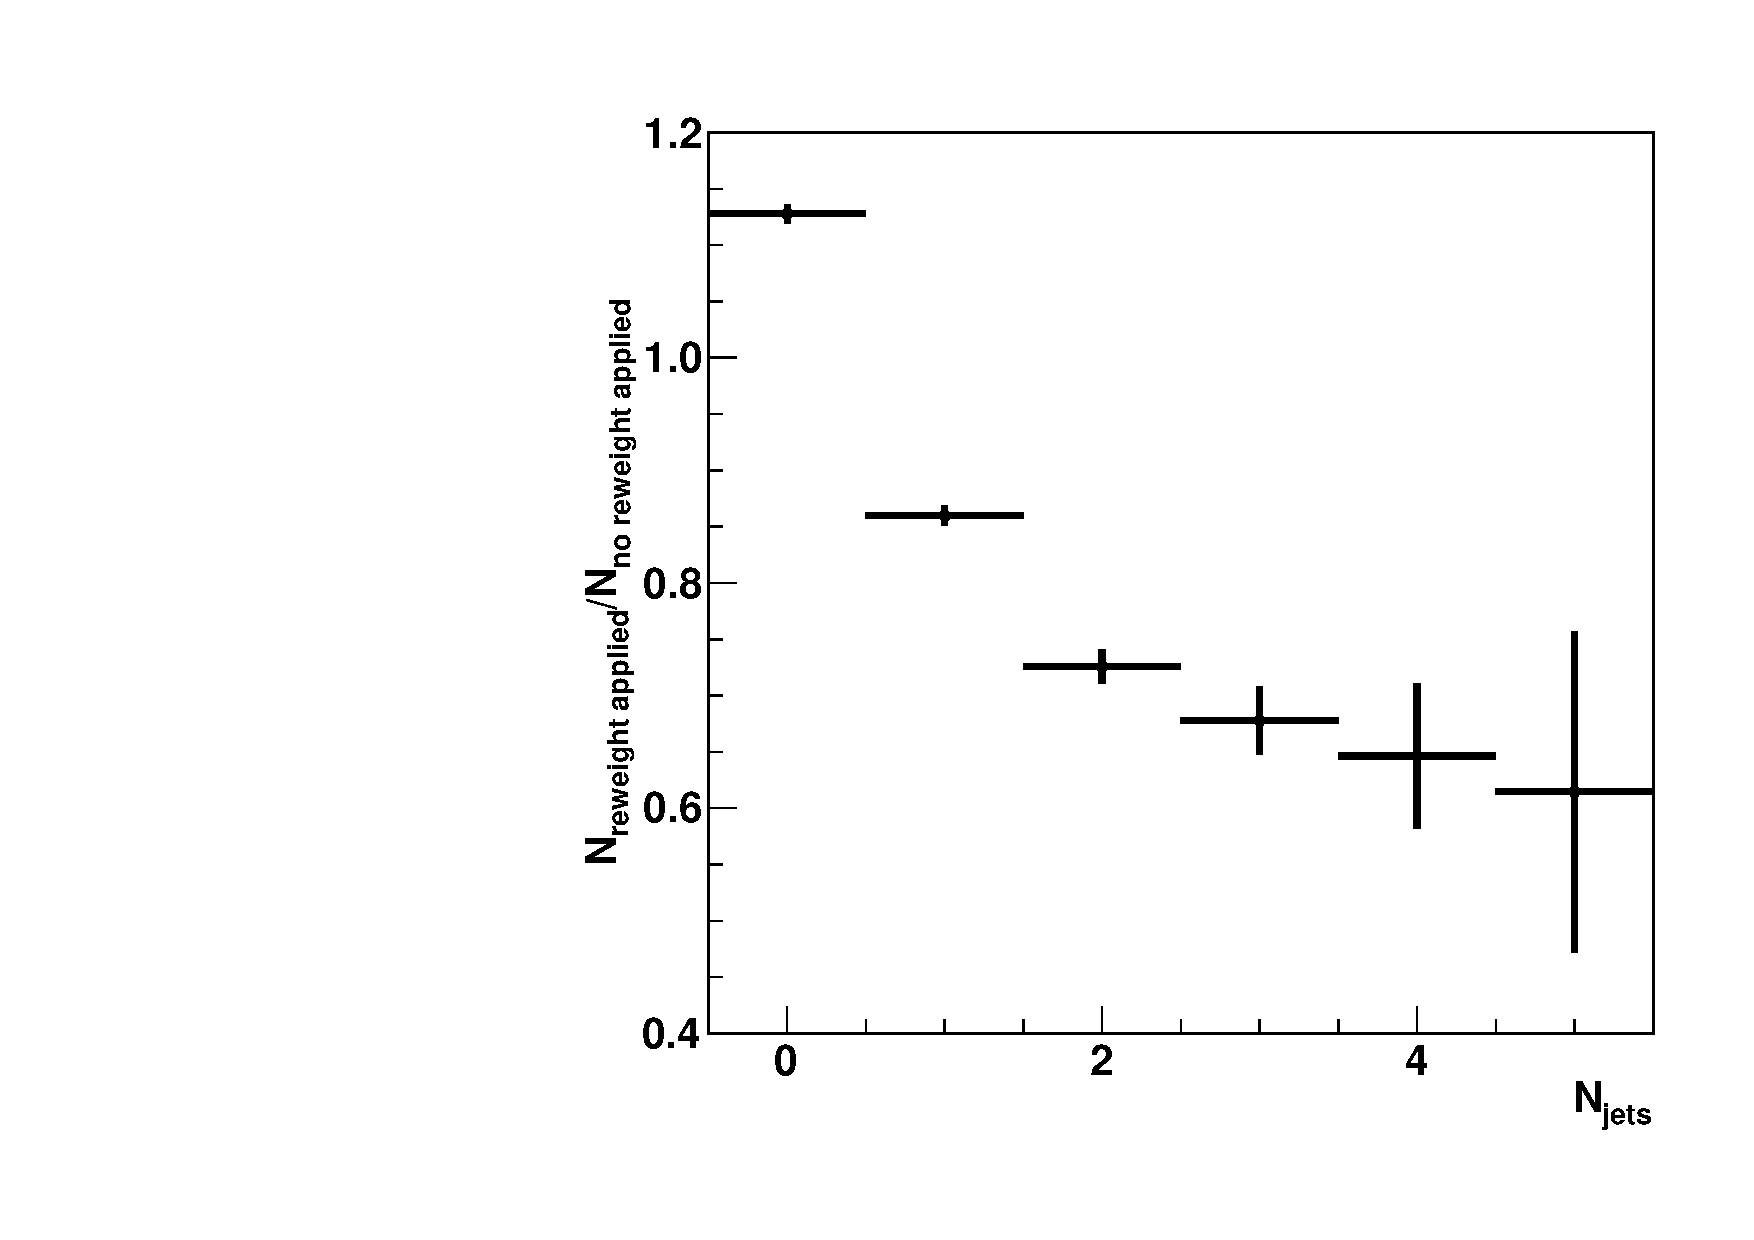
\includegraphics[width=0.49\textwidth]{figures/h160ww_njets_kfactor_ratio.pdf}} 
\caption{(a) Higgs transverse momentum spectrum as predicted by Powheg and the NNLO+NNLL calculation; (b) 
scale factors applied to each jet bin in the Powheg simulation.}
\label{fig:h160ww_pthiggs}
\end{center}
\end{figure}

\end{document}
